% !TEX program = pdflatex
% !TEX encoding = UTF-8 Unicode

% Plantilla, basada en la clase `scrbook` del paquete KOMA-script,  para la elaboración de un TFG siguiendo las directrices del la comisión del Grado en Matemáticas de la Universidad de Granada.

% Francisco Torralbo Torralbo

\documentclass[print, color]{ugrTFG}
\usepackage{float}

% VERSIÓN ELECTRÓNICA PARA TABLETA
% Cambiando la opción "print" por "tablet" generaremos un pdf adaptado para leerlo en tabletas de 9 pulgadas.

% -------------------------------------------------------------------
% INFORMACIÓN DEL TFG Y EL AUTOR
% -------------------------------------------------------------------

\newcommand{\miTitulo}{Estudio sobre la Efectividad del Positional Encoding en Transformers para Series Temporales y Diseño de Mecanismos Adaptados\xspace}

\newcommand{\miNombre}{Cristhian Moya Mota\xspace}
\newcommand{\miGrado}{Máster Universitario en Ciencia de Datos e Ingeniería de Computadores}
\newcommand{\miFacultad}{Escuela Técnica Superior de Ingenierías Informática y Telecomunicación}
\newcommand{\miUniversidad}{Universidad de Granada}

% Añadir tantos tutores como sea necesario separando cada uno de ellos mediante el comando `\medkip` y una línea en blanco
\newcommand{\miTutor}{
  Julian Luengo Martín \\ \emph{DECSAI}

  % Añadir tantos tutores como sea necesario.

  \medskip
  Diego Jesús García Gil \\ \emph{LSI}
}

\newcommand{\miMentor}{
	Ignacio Aguilera Martos \\ \emph{DECSAI}
}
\newcommand{\miCurso}{2024-2025\xspace}

\hypersetup{
  pdftitle={\miTitulo},
  pdfauthor={\textcopyright\ \miNombre, \miFacultad, \miUniversidad}
}

\begin{document}

\maketitle


% -------------------------------------------------------------------
% FRONTMATTER
% -------------------------------------------------------------------
\frontmatter % Desactiva la numeración de capítulos y usa numeración romana para las páginas


% !TeX root = ../tfg.tex
% !TeX encoding = utf8
%
%*******************************************************
% Summary
%*******************************************************

\chapter{Resumen}

En un mundo basado en los datos, donde diariamente generamos volúmenes inmanejables de información, nos enfrentamos a estructuras y semánticas muy diversas que condicionan las herramientas con el que podemos procesarlos y extraer información. Modelos recientes basados en Transformers~\cite{vaswani2023attentionneed} nos han permitido modelarlos y procesarlos de manera más sencilla, alcanzando objetivos prácticamente impensables hace unos años. Poseen una gran capacidad para capturar dependencias complejas y adaptarse a diferentes dominios, que abarcan desde su propósito original, el procesamiento de lenguaje natural, hasta otros muy diferentes, como las imágenes.\\
Entre todas estas estructuras, destaca un soporte concreto: las series temporales. Estas recogen información acerca de fenómenos muestreados a lo largo del tiempo, que pueden contener uno o más atributos que lo caracterizan, y que, de manera gráfica, nos permiten estudiar el comportamiento temporal de manera muy intuitiva. Hasta el momento, se han empleado diferentes técnicas clásicas basadas en la estadística, pero con el gran auge y versatilidad del Transformer, se ha tratado de adaptar esta herramienta para usarla como clasificador y predictor de futuros comportamientos de la serie.\vspace{0.35em}

La predicción a largo plazo, conocida en inglés como \textit{forecasting}, es uno de los principales frentes abiertos en la investigación. Esto se debe a que hasta el momento, las predicciones que requieren horizontes de larga duración se apoyaban en los valores predichos en un horizonte menor, lo cual fomentaba la acumulación errores de manera incremental hasta obtener resultados totalmente diferentes a lo que se esperaba. \vspace{0.35em}

Con esta nueva arquitectura, esta problemática parecía desaparacer, ya que estos pueden actuar de manera generativa con sus entradas, aprendiendo su estructura secuencial y siendo capaces de modelar su contenido. Sin embargo, a pesar de sus similaridades con el lenguaje natural, las series temporales difieren considerablemente de estas: disponemos de valores numéricos, que dependen de manera muy estricta de su instante temporal (timestamp), y cualquier ruptura en ese orden va en contra de la propia naturaleza de los datos.
Originalmente, los Transformers incorporan información adicional en sus secuencias de entrada para no perder el orden estructural de los datos. Para ello, enriquecen la entrada componiendo el embedding, construido por cada elemento de entrada más una serie de componentes que reflejan su posición dentro de la secuencia. Este mecanismo, llamado positional encoding, ha empleado hasta el momento mecanismos sencillos como la definición de posiciones mediante funciones trigonométricas, efectivas en texto, y que fueron heredadas en el nuevo dominio de las series temporales. Pero, en la práctica, se ha demostrado que no son un mecanismo efectivo ~\cite{zeng2022transformerseffectivetimeseries} para este ámbito.\vspace{0.35em}

Esto se debe a la falta de semántica del propio encoding, que no tiene en cuenta la información del entorno de cada instante temporal, más allá del orden absoluto establecido por la codificación original. En series temporales, la información local y la detección de patrones repetitivos es decisivo, y por tanto, es necesario crear un nuevo método de codificación capaz de modelar esta información con las series temporales como formato objetivo.\vspace{0.35em}

Este trabajo da un paso en ese aspecto, y propone una serie de métodos de codificación basados en un nuevo concepto novedoso: concatenar información adicional a las posiciones de entrada, de manera que cada instante medido llevo consigo información de contexto local que recoja comportamiento medio, desviación, y valores diferenciados con instantes anteriores, de forma que dos posiciones de igual naturaleza posean una codificación similar, y el modelo sea capaz de hacerlas corresponder. De esta forma, conseguimos mejorar el rendimiento de modelos en contextos estacionales, donde la serie repita su comportamiento periódicamente.\vspace{0.35em}

Adicionalmente, incorpora la idea de hacer coexistir a varias codificaciones, existentes en el estado del arte, en un mismo embedding, fruto sumatorio ponderado, de forma que estas se complementen entre sí, pero empleando pesos de ponderación aprendidos por el propio modelo, que reducen al mínimo la necesidad de especificación de parámetros de entrada.\\
Ambas propuestas han sido evaluadas empleando datasets de acceso abierto que recogen información sobre diferentes fenómenos, como sistemas transformadores de electricidad, sensores de maquinaria industrial y medidas de uso del transporte público, de manera que se predigan en horizontes a largo plazo en diferentes dominios, y se logre, como objetivo final, mejorar la predicción para optimizar la gestión de dichos sistemas.\vspace{0.35em}

Se han evaluado los resultados de todos los modelos, considerando tanto la eficiencia computacional como la mejora en las métricas de rendimiento. Con ello, ha sido posible identificar la propuesta que demuestra una mayor capacidad de generalización frente al conjunto completo de experimentos realizados. Los resultados obtenidos ofrecen márgenes de mejora razonables, de incluso entre un 10-30\%  en promedio, siendo en casos concretos de alta precisión una mejora de hasta el 90\% con respecto a los resultados de un modelo consagrado del estado del arte, como lo es Informer~\cite{zhou2021informerefficienttransformerlong}. 


% !TeX root = ../tfg.tex
% !TeX encoding = utf8
%
%*******************************************************
% Summary
%*******************************************************

\selectlanguage{english}
\chapter{Summary}

An english summary of the project (around 800 and 1500 words are recommended).

File: \texttt{preliminares/summary.tex}


% Al finalizar el resumen en inglés, volvemos a seleccionar el idioma español para el documento
\selectlanguage{spanish} 
\endinput


% !TeX root = ../tfg.tex
% !TeX encoding = utf8
%
%*******************************************************
% Declaración de originalidad
%*******************************************************

\thispagestyle{empty}

\hfill\vfill

\textsc{Declaración de originalidad}\\\bigskip

D./Dña. \miNombre \\\medskip

Declaro explícitamente que el trabajo presentado como Trabajo de Fin de Grado (TFG), correspondiente al curso académico \miCurso, es original, entendido esto en el sentido de que no he utilizado para la elaboración del trabajo fuentes sin citarlas debidamente.
\medskip

En Granada a \today 
\vspace{3cm}
\begin{center} 
Fdo: \miNombre 

\end{center}

\vfill

\cleardoublepage
\endinput

% !TeX root = ../tfg.tex
% !TeX encoding = utf8
%
%*******************************************************
% Declaración de originalidad
%*******************************************************
\cleardoublepage           % Forzar inicio en página nueva

\hfill\vfill

\textsc{Tutorización}\\\bigskip



D. \textbf{Julián Luengo Martín}, Profesor del Departamento de Ciencias de la Computación e Inteligencia Artificial
de la Universidad de Granada.
\vspace{0.5cm}

D. \textbf{Diego Jesús García Gil}, Profesor del Departamento de Lenguajes y Sistemas Informáticos de la Universidad de Granada.

\vspace{0.5cm}

\textbf{Informan:}

\vspace{0.5cm}

Que el presente trabajo, titulado \textit{\miTitulo},
ha sido realizado bajo su supervisión por \textbf{Cristhian Moya Mota}, y autorizamos la defensa de dicho trabajo ante el tribunal
que corresponda.

\vspace{0.5cm}

Y para que conste, expiden y firman el presente informe en Granada, \today.

\vspace{1cm}

\textbf{Los directores:}

\vspace{5cm}

\begin{center}
	\textbf{Julián Luengo Martín \ \ \ \ \ \ Diego Jesús García Gil}
\end{center}

\vfill

\cleardoublepage 
\endinput

% !TeX root = ../tfg.tex
% !TeX encoding = utf8

%*******************************************************
% Agradecimientos
%*******************************************************

\chapter*{Agradecimientos}

Agradecimientos (opcional, ver archivo \texttt{preliminares/agradecimiento.tex}).

\cleardoublepage
\endinput
                

% !TeX root = ../tfg.tex
% !TeX encoding = utf8

%*******************************************************
% Table of Contents
%*******************************************************
\phantomsection
\pdfbookmark[0]{\contentsname}{toc}

\setcounter{tocdepth}{2} % <-- 2 includes up to subsections in the ToC
\setcounter{secnumdepth}{3} % <-- 3 numbers up to subsubsections

\tableofcontents 

%*******************************************************
% List of Figures and of the Tables
%*******************************************************

    % *******************************************************
    %  List of Figures
    % *******************************************************    
    \phantomsection 
    % \listoffigures

    %*******************************************************
    % List of Tables
    %*******************************************************
    \phantomsection 
    % \listoftables
    
    %*******************************************************
    % List of Listings
    % The package \usepackage{listings} is needed
    %*******************************************************      
	  % \phantomsection 
    % \renewcommand{\lstlistlistingname}{Listados de código}
    % \lstlistoflistings 

\cleardoublepage


\listoffigures
\listoftables

% -------------------------------------------------------------------
% MAINMATTER
% -------------------------------------------------------------------
\mainmatter % activa la numeración de capítulos, resetea la numeración de las páginas y usa números arábigos

%\part{Primera parte} % Dividir un TFG en partes OPCIONAL

% Información relevante para la elaboración del trabajo.
\chapter{Introducción}

En este primer punto, describiremos de forma breve la motivación a realizar este TFM. Analizaremos la importancia de poseer herramientas capaces de realizar una predicción a largo plazo en series temporales (en inglés,\textit{ Long-term Time Series Forecasting},  LSTF), pero, sobre todo, centrándonos en un aspecto clave: la codificación posicional (\textit{Positional Encoding}, en adelante, PE), común a prácticamente todas las alternativas actuales del estado del arte. 

Procederemos a justificar su importancia, así como a formular los objetivos que se cubren con la realización de este trabajo.
\section{Motivación}

En la actualidad, los datos son uno de los bienes más preciados. Las telecomunicaciones nos han permitido alcanzar un volumen inimaginable de información digital, la cual no somos prácticamente capaces de procesar, y extraer conocimiento útil se convierte en una tarea complicada. Su gran variedad y modalidad hace necesario disponer de modelos multimodales cada vez más complejos para procesarlos, como los modelos fundacionales \cite{bommasani2022opportunitiesrisksfoundationmodels}, para tratar así de disponer de una herramienta cercana a ser capaz de procesar todo tipo de información.\\

Hemos podido apreciar grandes avances en el procesamiento de texto, con los grandes modelos de lenguaje como GPT, el cual se ha convertido en una herramienta que usamos habitualmente para resolver nuestras dudas. Ahora, incluso permite generar imágenes, vídeo y audio, y pensar profundamente las respuestas.\\

Sin embargo, estos no son los únicos tipos de datos que podemos emplear para aprender. Los datos basados en flujos, y las series temporales, son un recurso clave que podemos emplear para resolver multitud de problemáticas. Podemos predecir a largo plazo, clasificar fenómenos, o bien, incluso detectar anomalías. En este trabajo, nos centraremos sobre todo en la primera tarea y las dificultades que existen en este ámbito.

\subsection{Importancia de las Series Temporales}

Las series temporales son un tipo de datos caracterizados por una secuencia organizada en el tiempo. Generalmente, consisten en una o varias variables observadas a intervalos regulares, con el objetivo de registrar la evolución de un fenómeno. Suelen recogerse de forma periódica mediante sensores o procesos automatizados (por ejemplo, la temperatura de un motor medida por un termostato electrónico), aunque también pueden originarse de forma irregular, como en el caso de registros manuales. Es importante que, cuando se trata de múltiples variables, estas se muestreen con la misma frecuencia para facilitar su análisis y evitar la necesidad de técnicas de imputación, que podrían introducir distorsiones en los resultados.\\

El objetivo: utilizar estos datos para aprender qué ocurrirá en instantes futuros, realizando predicciones en un horizonte concreto sobre el que es desconocido su comportamiento. Sin embargo, es importante destacar que no todos los fenómenos pueden ser predichos aunque dispongamos de un conjunto de datos suficiente y adecuado. Es esencial que, para que la técnica sea efectiva, estemos ante una tarea de forecasting, es decir, de predicción de elementos futuros, pero pudiéndonos apoyar en información pasada para comprender el fenómeno que estamos estudiando. Por ejemplo, tratar de predecir la temperatura que hará en las próximas 2 horas, en intervalos de 15 minutos,es una tarea viable: disponemos de gran cantidad de recursos históricos, como la tendencia de las horas anteriores, y los valores históricos de días previos, o incluso, el comportamiento en años anteriores, que pueden ser útiles.\\

Pero también podríamos enfrentarnos a escenarios más complejos, como el que gestiona diariamente Red Eléctrica para estimar el consumo de electricidad y responder con los tipos de energía más adecuados, evitando tanto el exceso como el déficit en la red. Para ello, se apoyan no solo en datos históricos de consumo, sino también en la información en tiempo real proveniente de sensores y mediciones realizadas en distintas estaciones eléctricas, lo que permite anticipar fluctuaciones y minimizar problemas de sincronización. A esto se suman otros factores externos que pueden influir, como las condiciones meteorológicas o incidencias en redes interconectadas de países vecinos.
Tras la experiencia vivida en abril de 2025, queda en evidencia la importancia de esta tarea, ya que en caso de error, las consecuencias pueden ser muy graves: personas atrapadas en ascensores, hospitales en emergencia, problemas de tráfico, interrupción de la cadena de frío en los alimentos...
Las pérdidas económicas se estimaron entre 1.600 y 2.500 millones de euros.\\

Por tanto, disponer de buenas técnicas de estudio para series temporales es una herramienta clave en multitud de aplicaciones. Manualmente, podemos realizar aproximaciones posibles para casos sencillos, donde apreciamos un comportamiento repetitivo en el tiempo de la serie (estacionalidad) o un comportamiento estrictamente creciente o decreciente linealmente (tendencia). Sin embargo, cuando el problema se vuelve más complejo o involucra múltiples variables, recurrir a matemáticas simples o técnicas intuitivas ya no es suficiente. En estos casos, es necesario contar con herramientas más sofisticadas que permitan modelar el comportamiento de la serie de forma aproximada, pero lo más fiel posible a la realidad.\\

Es aquí donde entran en juego métodos ampliamente utilizados, como la descomposición de la serie en componentes fundamentales: tendencia, estacionalidad y ruido. Una de las técnicas estadísticas más reconocidas en este ámbito es ARIMA (AutoRegressive Integrated Moving Average) \cite{10.5555/574978}. Se basa en utilizar una ventana deslizable sobre la que ir calculando una media móvil, es decir, un intervalo de amplitud \textit{q} en torno a un valor central, el cual se va moviendo de izquierda a derecha para evaluar con todas las instancias de la serie, y en una componente autoregresiva, que trata de incorporar información de instantes anteriores al que se está evaluando (hasta p valores). También se integra la serie tantas veces como sea necesario para suavizar su comportamiento. De este modo, es posible generar predicciones razonables, siempre y cuando el problema cumpla con ciertas condiciones que abordaremos más adelante.\\

No obstante, incluso técnicas como ARIMA presentan limitaciones importantes, especialmente cuando se enfrentan a horizontes de predicción amplios. A medida que intentamos anticipar valores más alejados en el tiempo, el modelo se ve obligado a basarse cada vez más en sus propias predicciones previas en lugar de los datos observados, lo que provoca una acumulación progresiva de errores.\\

Esto plantea la necesidad de modelos más robustos, capaces de capturar dependencias de largo alcance y manejar múltiples variables de forma conjunta, tratando de minimizar el error evitando su acumulación. Podemos recurrir, como alternativa, a una de las herramientas ya empleadas en los grandes modelos de lenguaje que mencionamos anteriormente: los Transformers \cite{vaswani2023attentionneed}. Pero su uso no es directo; debemos de adaptar su funcionamiento a las series temporales, ya que estos modelos, originalmente diseñados para tareas de lenguaje natural, no conservan de manera adecuada la información temporal del orden de los datos.

\subsection{La dificultad de predicción a largo plazo: información posicional}

Para poder adaptar modelos basados en Transformers para lenguaje natural a series temporales,  es imprescindible introducir mecanismos de codificación posicional (positional encoding) que permitan al modelo interpretar correctamente la secuencia en el tiempo \cite{irani2025positionalencodingtransformerbasedtime}. Sin este componente, los Transformers serían incapaces de distinguir el orden de la entrada, lo cual es esencial para predecir correctamente la evolución de un fenómeno.\\

Encontrar una codificación eficiente, sencilla y coherente con la estructura de los datos se encuentra en continua búsqueda en el estado del arte, pero la mayoría de ellas presentan los siguientes inconvenientes:

\begin{itemize}
	\item \textbf{Falta de captura de la estructura}. En muchas ocasiones, se opta por utilizar codificaciones sencillas basadas en senos y cosenos, de la misma forma que se hace en procesamiento de lenguaje, pero de esta forma, estamos perdiendo información de patrones estacionales e información local de interés. Esto ocurre, por ejemplo, en modelos como Informer \cite{zhou2021informerefficienttransformerlong}, uno de los primeros en adaptar los Transformers a series temporales.

	\item \textbf{Dificultad para adaptarse a diferentes escalas temporales y falta de semántica}. Propuestas simples, como la ya mencionada codificación sinusoidal, pueden ser ineficientes cuando se busca trabajar con distintas granularidades temporales. Al tratarse de una codificación fija, sus valores no se ajustan al cambiar la frecuencia de muestreo (por ejemplo, de segundos a minutos) , ya que mantienen una amplitud y periodicidad predefinidas. Por otro lado, aproximaciones más complejas, como las basadas en convoluciones, intentan capturar patrones locales dentro de la secuencia, pero tienden a centrarse en un corto plazo, lo que dificulta la detección de relaciones de largo alcance o multiescala. Además, este tipo de codificación no incorpora explícitamente la semántica temporal (como la hora del día o el día de la semana), lo que limita su interpretabilidad y generalización en tareas donde esa información es relevante.
	

	\item \textbf{Complejidad}. Para paliar las dificultades de los métodos más simples, se han evaluado alternativas más complejas, que permiten aumentar el rendimiento: es el caso de Autoformer, que incorpora información autoregresiva al modelo, tomando así cierta similaridad con la componente AR de ARIMA; o bien, se proponen encodings basados en transformadas de Fourier. Pero estas aumentan la necesidad de cómputo y el tiempo necesario para su entrenamiento, lo cual hace surgir otra vertiente alternativa, basada en modelos más sencillos, como Reformer \cite{kitaev2020reformerefficienttransformer}, que trata de convertir la eficiencia cuadrática de los Transformers, a lineal. O Informer, que persigue lograr eficiencia \textit{n log n} mediante su ProbSparse Attention \cite{zhou2021informerefficienttransformerlong}. Pero, a veces puede conseguirse el efecto contrario: empeorar en exceso los resultados, a consta de un menor tiempo de entrenamiento e inferencia. Por ejemplo, en Informer, al muestrearse en atención solo ciertos vectores de entrada, perdemos información local que puede ser clave.
\end{itemize}

La misión de este trabajo se centra en tratar de encontrar una alternativa que sea capaz de mantenerse cercana a la semántica del problema, permitiendo adaptabilidad en cuanto a parámetros, y tratando de alcanzar un equilibrio entre eficiencia y rendimiento.\\

\section{Justificación}

Tras estudiar el problema, surge la necesidad de crear una alternativa adecuada a los modelos de codificación existentes, incorporando dentro de ella la semántica del propio problema, e información local que permita una mayor adaptabilidad de los modelos creados, reduciendo las tasas de error. Aunque este objetivo ya es tratado por diversos modelos y líneas de investigación del estado del arte, en este trabajo buscamos replantear el positional encoding para que sea adaptable y capaz de incorporar información global y local, dando mayor importancia a una u otra en función de la entrada dada.\\

Todo esto se plantea aprovechando el conocimiento adquirido a partir de técnicas más clásicas, como ARIMA, e incorporando información estadística que resulte comprensible para prácticamente cualquier persona que utilice el modelo. De este modo, aunque se recurra posteriormente a modelos profundos como los Transformers, la codificación posicional introducida  al inicio en los datos puede ser ajustable y fácilmente interpretable en función del contexto del problema.\\
 
Hasta ahora, gran parte de los esfuerzos se han centrado en adaptar soluciones desarrolladas originalmente para otros dominios, principalmente el procesamiento de lenguaje natural, al contexto de las series temporales. Sin embargo, estas adaptaciones no siempre se alinean completamente con las particularidades de los datos temporales, lo que puede derivar en pérdidas de información relevantes o en un rendimiento subóptimo. Esta desconexión pone de relieve la necesidad de desarrollar codificaciones específicamente diseñadas para capturar la estructura temporal propia de este tipo de datos. En este documento, abordaremos esta problemática desde una perspectiva crítica, comparando distintos métodos existentes y proponiendo nuevas soluciones, algunas de ellas híbridas, que buscan mejorar la representación temporal en modelos basados en Transformers.

\section{Objetivos}

Teniendo en cuenta los conceptos descritos anteriormente, y analizando el estado del arte en la actualidad, vemos justificada la necesidad de encontrar nuevas codificaciones posicionales con el objetivo de conseguir:

\begin{enumerate}
	\item Realizar una revisión exhaustiva del estado del arte sobre positional encoding y su aplicación en modelos Transformer para series temporales, estudiando el funcionamiento de las diferentes técnicas y extrayendo el conocimiento útil para crear nuevas alternativas.
	
	\item Analizar las propuestas originales de positional encoding adaptadas a series temporales, realizando un análisis crítico y explorando las diferentes vías alternativas.
	
	\item Evaluar sistemáticamente la efectividad de los positional encoding estándar en tareas de forecasting sobre benchmarks de series temporales, haciendo uso de varios conjuntos de datos de diferente procedencia y estructura.
	
	\item Establecer criterios claros para el diseño de nuevas codificaciones que permitan encontrar nuevas formas de incorporar información útil, pero además sirvan como guía para investigaciones futuras, identificando buenas prácticas, limitaciones comunes y condiciones bajo las cuales cada enfoque resulta más adecuado.
	
	\item Comparar el impacto de las distintas codificaciones posicionales no solo en la precisión de las predicciones, sino también en aspectos como la capacidad de generalización y su eficiencia computacional.

\end{enumerate}

En este documento, se recoge el estudio del estado del arte actual, realizando un estudio crítico y comparativo de las diferentes propuestas, haciendo también hincapié en el propio funcionamiento de los Transformer y como afecta a la codificación y procesado de la información. Se buscará, como ya se ha mencionado, crear un resumen con diferentes técnicas, nuevas y otras conocidas, que por separado o en su conjunto, de forma híbrida, propongan soluciones adecuadas a diferentes conjuntos de datos provenientes del mundo real.\\

Adicionalmente, se proporciona el repositorio en GitHub\footnote{Repositorio: https://github.com/hexecoded/tfm} que contiene todo el código desarrollado, así como las referencias a los conjuntos de datos utilizados. Este recurso se mantiene accesible con el objetivo de facilitar su análisis, reutilización y posible mejora en trabajos futuros.

\chapter{Tendencias y Estado del arte}

Antes de adentrarnos de lleno en el análisis del problema y la realización de nuevas metodologías, es necesario estudiar y comprender el estado actual de esta temática en el estado del arte. Debido a que no se ha visto tan explotada como otros ámbitos de la IA, como es el caso de los modelos convolucionales o el aprendizaje automático supervisado tabular, podemos encontrar continuos cambios y nuevas vertientes que pueden inspirarnos a la hora de abordar el problema.

Hasta hace una década, buena parte de las técnicas diseñadas especialmente para series temporales y predicción a largo plazo, se basan principalmente en la descomposición las mismas en subcomponentes mucho más sencillas de procesar, las cuales pueden seguir un enfoque similar a divide y vencerás: descomponer la red en diferentes elementos, y mediante un mecanismo de agregación (aditivo, multiplicativo, o estadístico), recomponer la solución a la tarea. Sin embargo, se trata de una estrategia últimamente menos utilizada, en decadencia a favor de nuevas técnicas \\

Actualmente, una de las principales tendencias consiste en adaptar modelos originalmente desarrollados para otras modalidades. Un ejemplo de ello es el uso de convoluciones, ampliamente utilizadas en visión por computador, con el objetivo de capturar patrones locales en las secuencias y reducir la dimensionalidad del modelo. Previamente, también se han explorado arquitecturas recurrentes, como las Recurrent Neural Networks (RNN) y sus variantes más avanzadas, como las Long Short-Term Memory (LSTM) \cite{6795963}, aunque estas presentaban ciertas limitaciones en cuanto a capacidad de paralelización y en la modelización de relaciones temporales de mayor alcance, ya que para lograrlo aumentaba en exceso el tamaño de la red para incorporar más conexiones.\\

Más recientemente, ha ganado protagonismo la adaptación de mecanismos provenientes del procesamiento de lenguaje natural, en particular los Transformers, debido a su capacidad para modelar dependencias a largo plazo de forma eficiente. Además, comparten una motivación estructural con las series temporales: la necesidad de preservar una secuencia ordenada y coherente en la entrada, lo que permite aprovechar su arquitectura basada en atención para tareas de predicción.\\

A continuación, nos adentraremos de lleno en dichas propuestas, con el fin de aclarar, en primer, los conceptos clave acerca de las series temporales, y además, entender las problemáticas que surgen durante su procesado.

\section{Procesamiento básico de Series Temporales}

En la introducción, se han presentado brevemente las características fundamentales de las series temporales: su estructura temporal, caracterizada por muestreo, la importancia del orden de medición, y la necesidad de mantener las relaciones temporales para lograr aprender de forma efectiva.\\

Pero, en esta sección, profundizaremos en los aspectos clave del preprocesamiento necesario para su análisis de manera más formal, ya que a diferencia de otros tipos de datos, las series temporales requieren una atención especial a la dimensión temporal, y cualquier alteración en su estructura puede afectar directamente la capacidad del modelo para aprender los patrones subyacentes en ella. Por ello, es fundamental centrarnos en cuestiones como la frecuencia de muestreo, la consistencia temporal, el tratamiento de valores faltantes, y la normalización de las variables.

\subsection{Modelos basados en descomposición}

Las series temporales pueden exhibir una gran cantidad de patrones y comportamientos, los cuales son interesantes de estudiar y visualizar con claridad para estudiar que posible enfoque seguir a la hora de resolver el problema. Diferenciando cada una de las partes, podemos tratar de resolver cada una de ellas por separado, y posteriormente, construir un modelo agregado capaz de solucionar nuestro problema.\\

Frecuentemente, podemos encontrar 3 comportamientos, los cuales son fácilmente identificables incluso gráficamente, que nos permiten obtener información bastante valiosa acerca del problema que estamos estudiando, y nos facilitan la decisión de escoger la técnica adecuada:

\begin{itemize}
	\item \textbf{Tendencia}. Es el movimiento de los valores de serie a largo plazo, es decir, el comportamiento mostrado por los datos a la hora de estudiar su progresión desde el inicio de la serie hasta su final. El objetivo es encontrar si esta mantiene una dirección, de manera general, en su periodo de muestreo, buscando si sigue un comportamiento creciente, decreciente o constante, al igual que en el caso de estudio de monotonía clásico en funciones. Normalmente, se representan mediante comportamientos sencillos, y no se ven afectadas por grandes variaciones o el impacto de otras componentes de la serie, como variables aleatorias u otros factores externos. Normalmente, podemos modelarla haciendo uso de funciones elementales, como ecuaciones lineales o funciones exponenciales, logarítmicas o polinomiales.
			
	A veces, se requieren procesos de suavizado para así poder eliminar el efecto de otras componentes ruidosas que rodean la tendencia real de la serie. Esto se puede conseguir, de manera similar a la convolución, desplazando una ventana a lo largo de la serie, de manera que los valores dentro de ella sean suavizado. La forma más habitual de lograrlo es con una media móvil, la cual, cuanto mayor amplitud tenga, mayor reducción de ruido conseguiremos.
	
	En la figura \ref{trend}, podemos ver un ejemplo de su cálculo representado gráficamente sobre el dataset Air Passengers \cite{box1976time}.
	
	\begin{figure}[h] %con el [H] le obligamos a situar aquí la figura
		\centering
		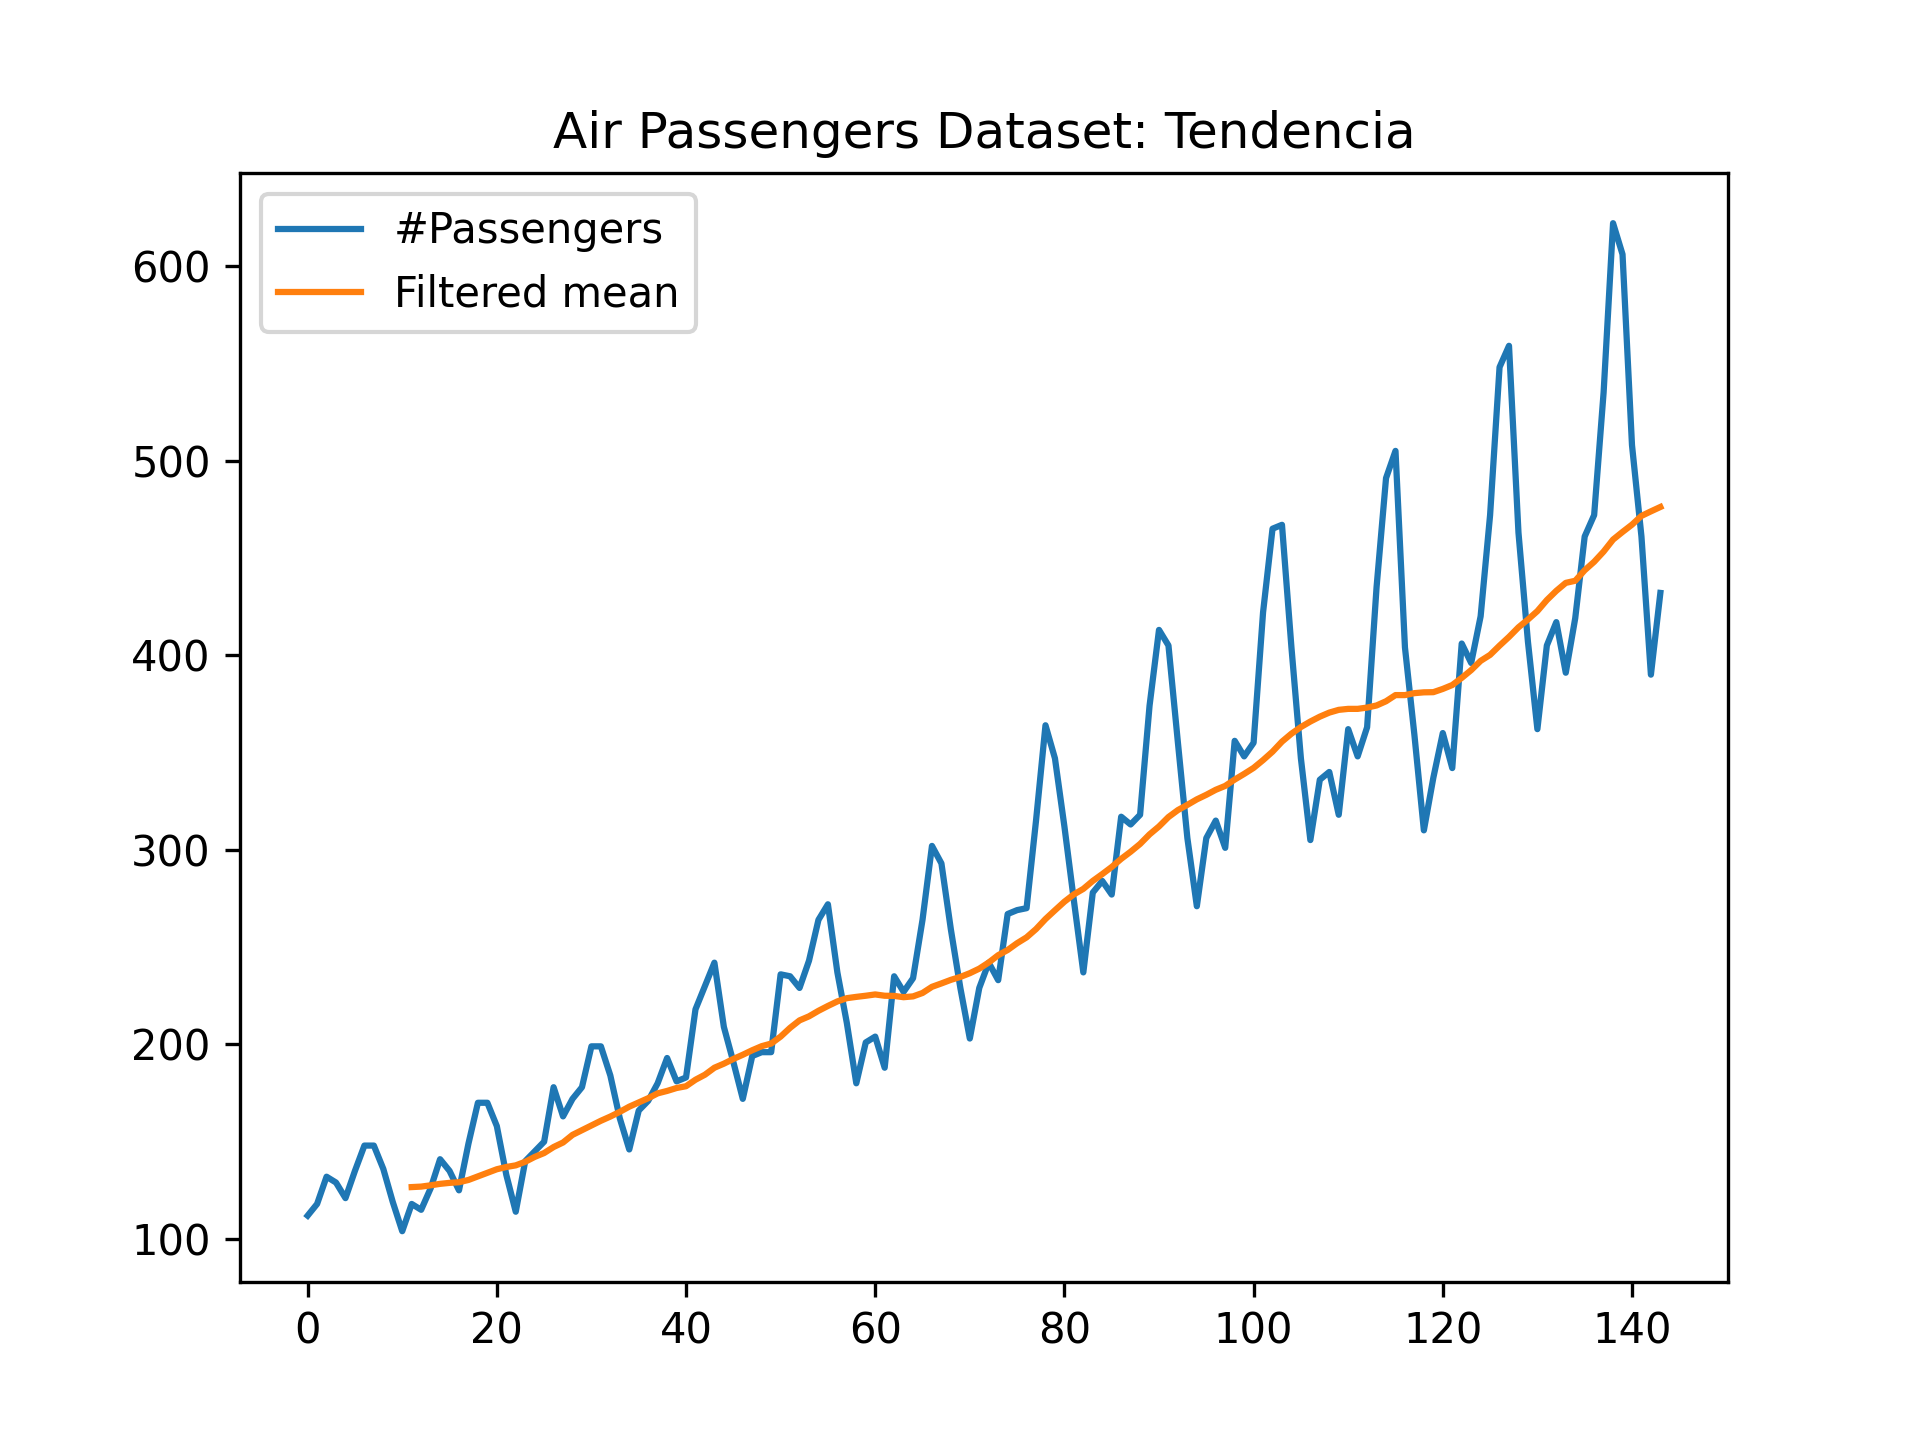
\includegraphics[scale=0.6]{img/trend}
		\caption{Estudio de la tendencia en el dataset Air Passengers}
		\label{trend}
	\end{figure}  	
	
	\item \textbf{Estacionalidad}. Son fluctuaciones periódicas y predecibles dentro de la serie temporal, las cuales siguen una determinada frecuencia y que pueden ser fácilmente modelables una vez se observa al menos un periodo. Normalmente, coinciden con unidades de medida de calendario, pudiendo encontrar así frecuecias semanales, mensuales, trimestrales, anuales... etc. Normalmente, son un factor visualmente sencillo de identificar, el cual apenas varía ente períodos, y que nos permite obtener información muy valiosa para el modelado.
	
	Podemos encontrar este comportamiento, por ejemplo, en los desplazamientos realizados durante las épocas vacionales: podremos observar un patrón de crecimiento en estas en Navidad y las vacaciones de verano, principalmente julio y agosto; y en el resto de meses el comportamiento será a la baja. Y eso ocurrirá con un período anual, ya que dichas fechas se ubican siempre en el mismo lugar. Diferente caso sería con Semana Santa, ya que su fecha no es coincidente todos los años y no cumple al 100\% de estacionalidad como las otras dos, ya que aunque es acotable en calendario, no es exactamente coincidente anualmente.
	
	En el caso del dataset anterior, se puede observar esta estacioalidad claramente (figura \ref{season})
	
		\begin{figure}[h] %con el [H] le obligamos a situar aquí la figura
		\centering
		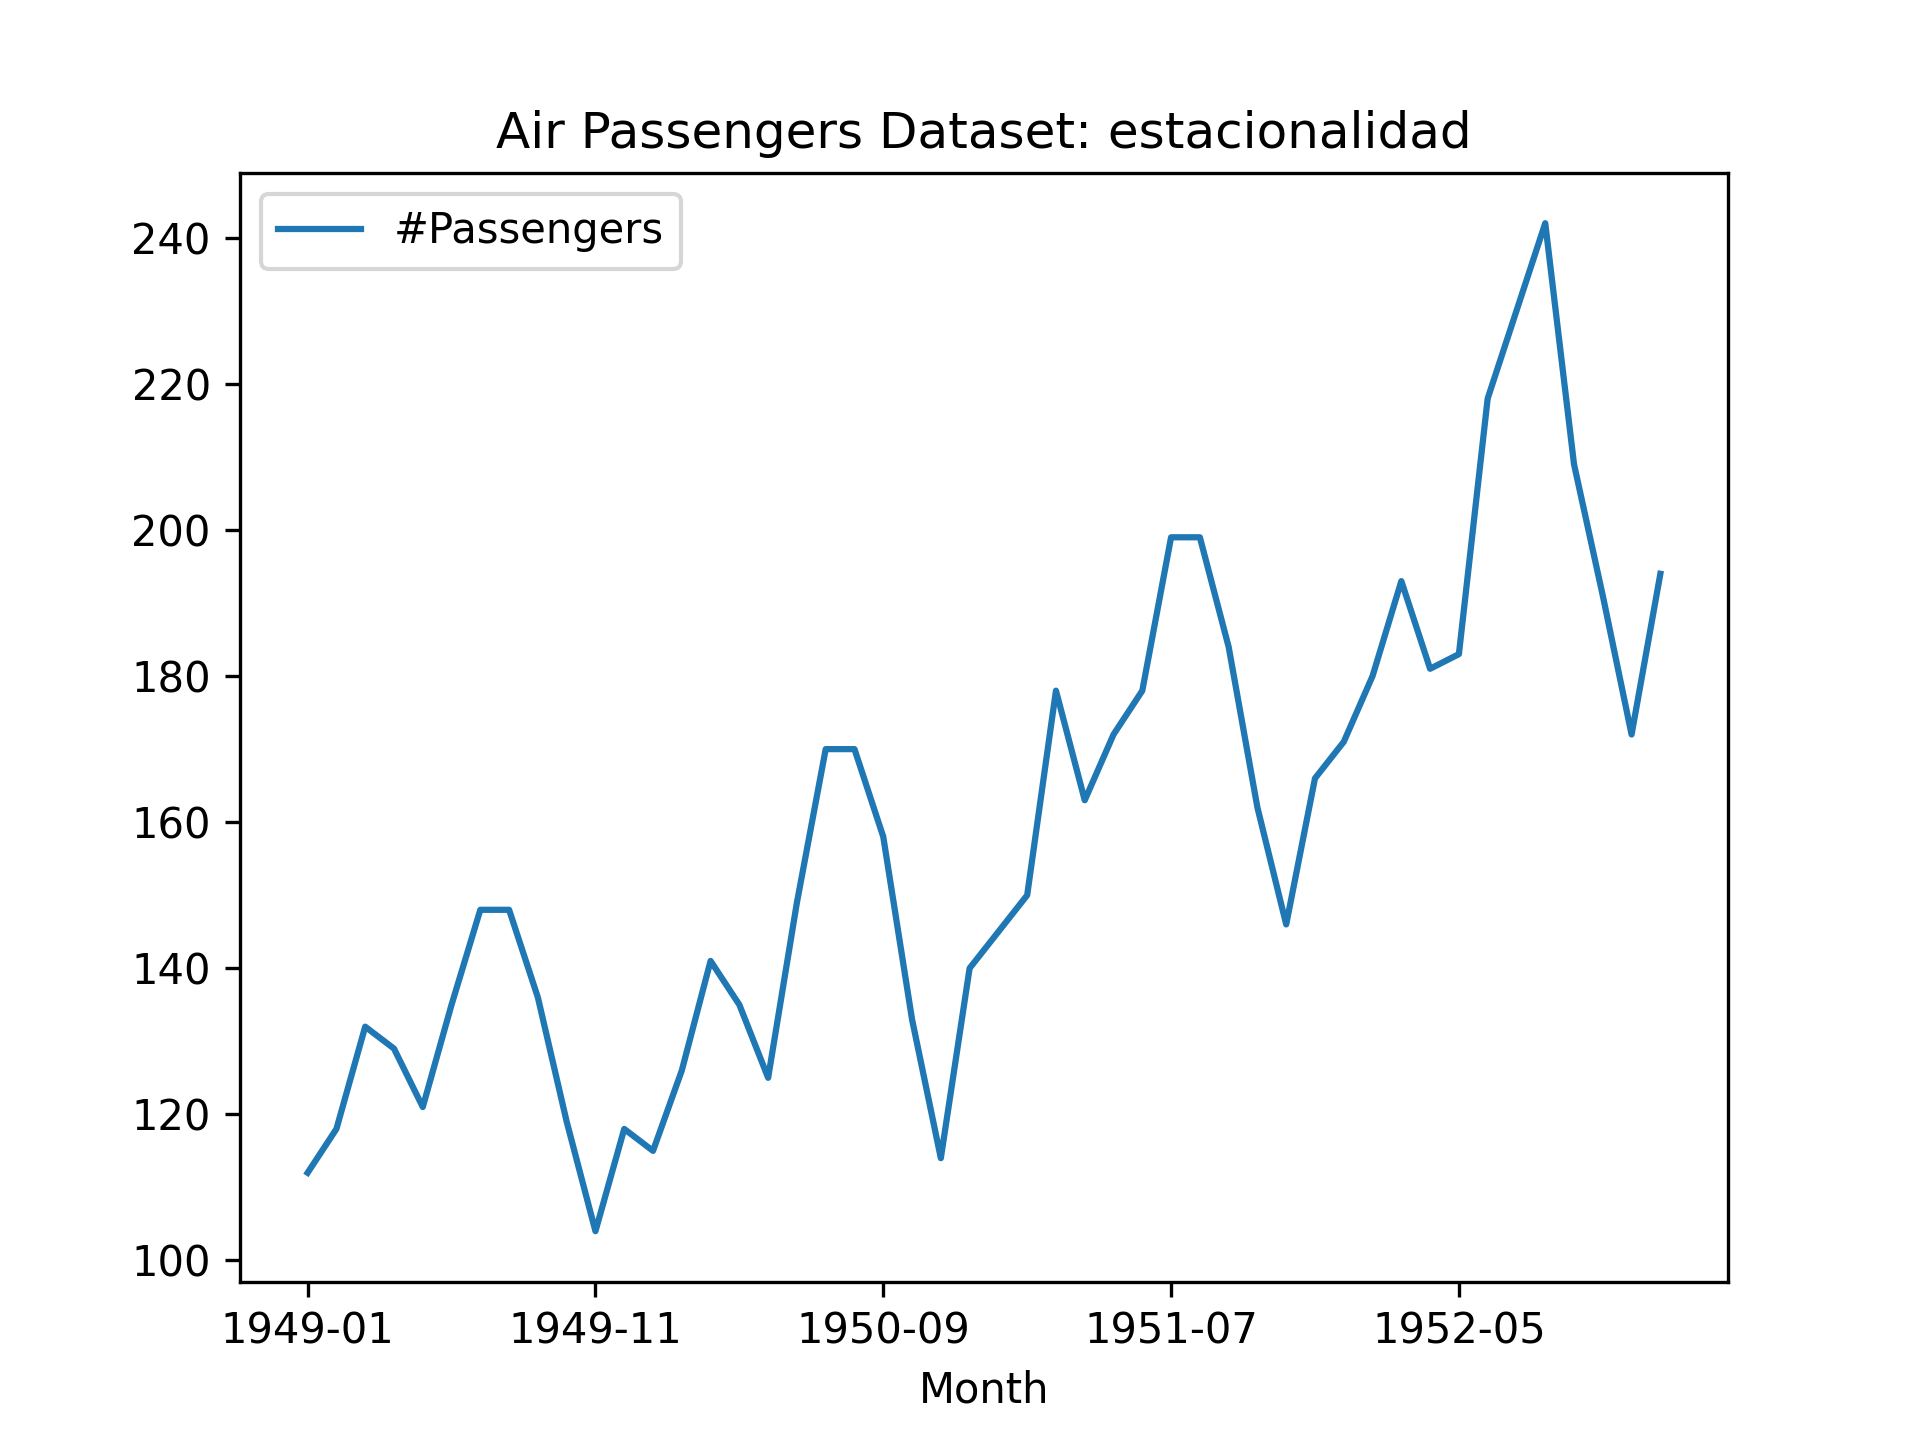
\includegraphics[scale=0.6]{img/season}
		\caption{Estudio de la estacionalidad en el dataset Air Passengers}
		\label{season}
	\end{figure}  	
	
	\item \textbf{Ciclo}. Son también fluctuaciones de la serie temporal, pero, a diferencia de ser regulares, siguen un período irregular de logitud fija. Normalmente, está vinculado a eventos que no están especialmente vinculados a fenómenos de calendario. El ejemplo más representativo podría ser la tendencia de crecimiento económico de un país, o el comportamiento de las acciones en bolsa de una sociedad anónima. 
	
	En la figura \ref{ciclo} podemos un ejemplo de este comportamiento con los permisos concedidos para la construcción de viviendas en EEUU \cite{techcharts2012housing}, donde no podemos encontrar patrones claros como en Air Passengers.
	
			\begin{figure}[H] %con el [H] le obligamos a situar aquí la figura
		\centering
		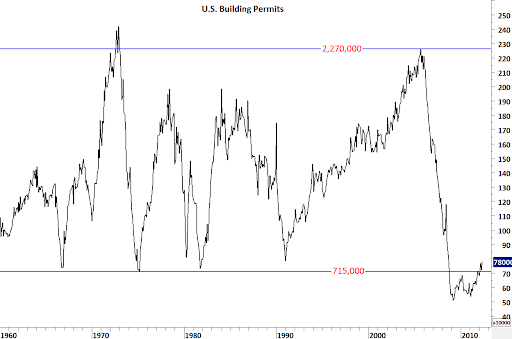
\includegraphics[scale=0.55]{img/ciclo}
		\caption{Estudio de ciclos en USA building permits}
		\label{ciclo}
	\end{figure}  	
	
\end{itemize}

Una vez comprendidos estos conceptos, podremos utilizar su información para decidir qué modelo se adapta mejor a nuestro problema y además tratar de modelar la tendencia y la estacionalidad. Anteriormente, mencionamos la gran utilidad de modelos como ARIMA, que funciona bajo este concepto. Pero no se trata del único modelo existente bajo este paradigma, sino uno de los más utilizados. En función del mecanismo de agregación de la solución, podemos clasificar las técnicas en dos grupos:

\begin{itemize}
	\item \textbf{Descomposición aditiva}. Realiza una separación de la serie temporal varias componentes, las cuales son modeladas por separado y sumadas entre si para dar lugar a la función predicha final (ecuación \ref{sum}). Es la más sencilla de usar en casos simples. Es indicada cuando las fluctuaciones estacionales por las variaciones entorno a la tendencia no varían con el valor de la serie temporal, es decir, pueden prácticamente mantenerse entre a lo largo de toda la serie sin apenas cambios. En general, se usa cuando los elementos no depende los unos de otros.
	
	\begin{equation}
	y(t) = T(t) + S(t) + C(t) + E(t)
	\label{sum}
	\end{equation}

	\item \textbf{Descomposición multiplicativa}. Se utiliza esta alternativa cuando las diferentes componentes dependen en nivel general de la serie (ecuación \ref{prod}). Es el caso de las series en las cuales los aumentos en la tendencia provocan aumentos también los picos de las tendencias estacionales o los ciclos.  Por ejemplo, en el dataset de Air Passengers, el comportamiento que se da es de este tipo.
	
	\begin{equation}
		y(t) = T(t) \times S(t) \times C(t) \times E(t)
		\label{prod}
	\end{equation}
	
\end{itemize}

Donde, en ambos casos:

\begin{itemize}
	\item \textit{T(t)}: Componente de la tendencia
	
	\item \textit{S(t)}: Componente estacional
	
	\item \textit{C(t)}: Componente cíclica
	
	\item \textit{E(t)}: Componente aleatoria y error
\end{itemize}

La elección de cada método depende, por tanto, de los datos, y nos beneficiaremos, como ya hemos visto a lo largo de la definición, de una adecuada visualización de los mismos cuando sea posible.

A continuación, definiremos en mayor detalle 3 de los algoritmos basados en descomposición más usados: STL \cite{cleveland1990stl}, ARIMA \cite{box1970time} y Prophet \cite{taylor2018prophet}.

\subsubsection{STL}

Esta técnica, llamada \textit{Seasonal Time-Series Decomposition}, nos permite descomponer la serie en partes más sencillas de modelar, separando la serie en tres componentes básicas: tendencia, estacionalidad y resto, siguiendo así el esquema visto anteriormente. De esta forma, podemos comprender en mayor detalle cómo evolucionan los valores a lo largo del tiempo, y comprender mejor cómo modelar su comportamiento. 

\paragraph{Funcionamiento}


Para obtener un modelo para cada una de ellas,  normalmente se sigue un proceso de 3 pasos que nos permite aislar la información.

\begin{enumerate}
	\item \textbf{Extracción de la tendencia}. Se comienza extrayendo la tendencia de la serie para así obtener el comportamiento subyacente de la misma, y saber si es creciente, decreciente o se mantiene constante. En este algoritmo, se consigue mediante un proceso de suavizado, llamado \textit{Locally Estimated Scatterplot Smoothing} (Loess) de manera iterativa. Para ello, primero se comienza aplicando Loess, de manera que se suavizan los valores realizando una regresión no parámetrica, donde se observan los valores cercanos a cada timestamp de manera que se realiza un promedio que reduce las diferencias en el entorno. Si la serie es muy compleja o ruidosa, es posible que sea necesario repetir este proceso varias veces, por lo que se convierte en un proceso iterativo, utilizando tamaños mayores de ventana entorno a cada valor.
	
	Dicha ventana se estima a través de pesos, los cuales se ven reducidos cuanto más alejados al valor están. Estos se rigen por el valor de amplitud \textit{h}, que recogen las ecuaciones clásicas de la regresión de Loess. Dado un conjunto de datos \((t_i, y_i)\), el valor suavizado en \( t_0 \) se calcula como:
	
	\[
	\hat{y}(t_0) = \mathbf{x}_0^\top \hat{\boldsymbol{\beta}}(t_0)
	\]
	
	donde \(\hat{\boldsymbol{\beta}}(t_0)\) se obtiene minimizando la suma ponderada de errores:
	
	\[
	\hat{\boldsymbol{\beta}}(t_0) = \arg\min_{\boldsymbol{\beta}} \sum_{i=1}^n w_i(t_0) \left(y_i - \mathbf{x}_i^\top \boldsymbol{\beta}\right)^2
	\]
	
	Los pesos \( w_i(t_0) \) dependen de la distancia temporal y se definen, habitualmente, con el kernel tricúbico:
	
	\[
	w_i(t_0) = \left(1 - \left|\frac{t_i - t_0}{h}\right|^3\right)^3, \quad \text{para} \quad |t_i - t_0| < h
	\]
	
	El valor arrojado será 0 fuera del intervalo, y un valor entre 0 y 1 dentro de él, seleccionando así la relevancia de cada punto respecto a sus valores del entorno.
	
	\item  \textbf{Extracción de la estacionalidad}. Para extraer la estacionalidad, debemos aislarla de la tedencia que modelamos en el paso anterior. Para ello, basta con restar dicha componente a la serie original, y así disponer ahora únicamente del los patrones estacionales y el ruido. 
	$$y'(t) = y(t) - trend(t)$$
	
	A partir de aquí, debemos dividir la serie sin tendencia en subseries estacionales, agrupando los datos según la posición que ocupan dentro del ciclo; por ejemplo, si identificamos patrones con frecuencia mensual, se agruparían todos los valores correspondientes al mismo mes en años distintos, y sobre cada una de estas subseries se aplica un suavizado Loess de forma individual. Así, podremos capturar con precisión el patrón que se repite en cada estación, de manera similar a un promedio. Gracias a este proceso, podremos reconstruir una componente estacional coherente con las variaciones periódicas observadas en nuestro conjunto de datos, al que denominaremos \textit{s(t)}.
	
	\item \textbf{Obtención del resto}. Una vez extraídas tanto la tendencia como la estacionalidad, la componente residual se obtiene simplemente como la diferencia entre la serie original y la suma de las dos componentes anteriores:
	$$r(t) = y(t) - trend(t) - s(t)$$
	 Esta parte representa la variabilidad no explicada por los patrones sistemáticos de largo plazo ni por los ciclos periódicos, e incluye tanto el ruido aleatorio como cualquier información no capturada por el modelo. Si bien no es modelable, es muy útil para identificar si la serie es correctamente modelable por este método, ya que si observamos demasiada información en esta componente, nos está indicando que una parte importante de la información no está siendo recogida. Lo deseable es la que la varianza descrita sea la mínima posible. Sin embargo, hay algunos casos en los que encontrar puntos extremos es de utilidad, y se trata de la búsqueda de valores anómalos. Si la serie restante permanece estable y con poca varianza, a excepción de ciertos puntos, puede ser de interés estudiar qué ocurrió en dichos instantes, ya que su comportamiento se sale del comportamiento habitual modelado.
\end{enumerate}

En su publicación original, podemos encontrar un ejemplo de ejecución sobre el conjunto de datos \textit{Daily Carbon Dioxide Data} (ver figura \ref{stl}), que recoge información sobre las emisiones de $CO_2$ desde el 17 de abril de 1974 hasta el 31 de diciembre de 1986, y permite observar la información recogida por cada una de las componentes.

\begin{figure}[!htp] %con el [H] le obligamos a situar aquí la figura
	\centering
	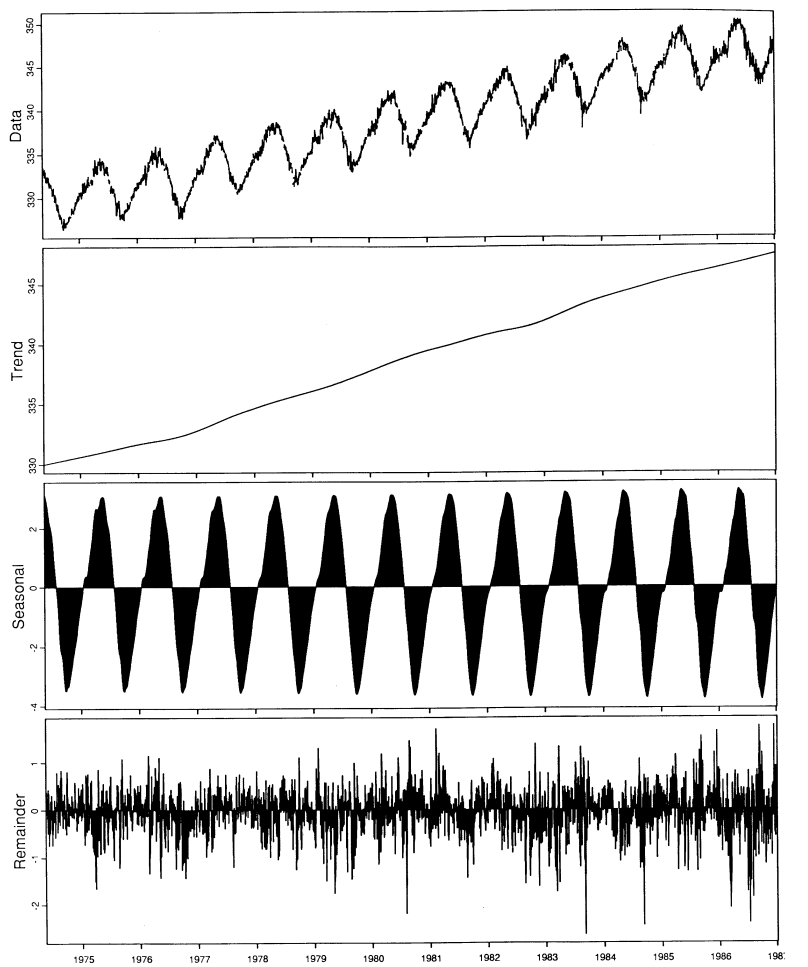
\includegraphics[scale=0.35]{img/stl}
	\caption{STL: Ejemplo de caso de estudio, Daily Carbon Dioxide Data \cite{cleveland1990stl}}
	\label{stl}
\end{figure}  	

En este caso, podemos apreciar visualmente una serie fácilmente modelable por este enfoque, ya que la curva describe una tendencia creciente bastante clara, y los periodos estacionales están bastante bien delimitados y no se ven influenciados por el crecimiento recogido en la tendencia. Es un ejemplo perfecto para el uso de los modelos basados en descomposición aditiva.

\paragraph{Conclusiones}


STL supuso una buena base para modelos posteriores, pero esta forma de modelado presenta varias limitaciones, que acotan su funcionamiento a problemas simples:

\begin{itemize}
	\item Sólo se limita a descomponer series de naturaleza aditiva, por lo que aquellas en las que las diferentes componentes se vean influenciados entre sí requerirán técnicas propias de modelos multiplicativos.
	\item Pueden perderse gran cantidad de detalles explicados por los datos, debido a la configuración del parámetro de suavizado. Si alisamos de más la serie, podemos estar perdiendo información clave acerca de nuestro problema, dejando completamente de lado ciertos comportamientos sutiles, lo cual aumenta la tasa de error. Debemos escoger adecuadamente los valores al aplicar Loess.
	\item Es costoso computacionalmente en caso de series de larga duración, ya que el cálculo de aplicar el kernel se hace para cada punto en cada iteración sobre el conjunto de datos, tanto para encontrar la tendencia como para luego generalizar la estacionalidad.
\end{itemize}

Pero, sin lugar a dudas, la principal desventaja de este método es que no consigue por sí solo lo que deseamos resolver en este trabajo: predecir, sobre todo, a largo plazo. STL es un procedimiento muy útil que nos permite entender el comportamiento de los datos, y descomponerlo para comprender el funcionamiento de cada componente, pero no es posible por sí solo realizar predicciones. Dependemos del apoyo de otros procedimientos que nos permitan estimar , basándonos en este historial, la progresión de las componentes extraídas como la tendencia (modelable por regresión), y la estacional, la cual podría ser evaluada de manera simplificada por su valor medio histórico por intervalo.\\

Esto lo hace en un método interesante desde el punto de vista de análisis, y que permite dar lugar a modelos que sí son capaces de estimar predicciones futuras, pero no es una herramienta por sí sola que nos permita resolver la tarea que nos concierne en este trabajo.

\subsubsection{ARIMA}

Basándonos de nuevo en el método de descomposición de series, podemos encontrar el modelo \textbf{ARIMA} (\textit{AutoRegressive Integrated Moving Average}) una técnica estadística ampliamente utilizada para el modelado de series temporales univariantes. Como ya adelantamos en la introducción del proyecto, su estructura se basa en la combinación de tres componentes principales: una parte autoregresiva (AR), una parte integrada (I) y una parte de media móvil (MA). Cada una de estas partes permite capturar diferentes aspectos del comportamiento temporal de los datos.

\paragraph{Componente de Integración}


Por integración, entendemos el número de veces que es necesario integrar la serie temporal original para que esta se vuelva estacionaria.  De manera resumida, una serie estacionaria es aquella cuyas propiedades estadísticas, como la media, la varianza y la autocorrelación entre valores, se mantienen constantes a lo largo del tiempo,  como ya vimos en la definición de los modelos aditivos.\\

La diferenciación nos permite eliminar tendencias o patrones sistemáticos de crecimiento o decrecimiento, facilitando el modelado de las componentes autoregresivas (AR) y de media móvil (MA). A pesar de que su nombre nos pueda insinuar un proceso complejo de integración analítica, al realizarse sobre valores numéricos, no es más que una diferencia de valores:

\[
y'_t = y_t - y_{t-1}
\]

Este proceso puede aplicarse tantas veces como sea necesario para lograr estacionariedad. Dicho número de repeticiones viene controlado por el valor de orden \( d \), que indica el número de veces que se ha diferenciado la serie. En general, el modelo ARIMA supone que tras aplicar \( d \) diferencias, la serie resultante \( y^{(d)} \) puede ser modelada por un proceso estacionario ARMA(\(p,q\)). Por tanto, el componente \textit{I} de ARIMA es un procesamiento indispensable de la serie cuando no se cumpla el requisito de estacionariedad, y permitirá calcular sobre la serie resultante las componentes AR y MA con mayor facilidad. \\

Para saber cuando deja de ser necesario aplicar el proceso iterativo de integración, podemos hacer uso de dos posibles mecanismos: uno gráfico, basado en el gráfico de autocorrelación de valores, y otro estadístico, basado en el test de Dickey-Fuller aumentado (ADF).

\begin{itemize}
	\item El análisis gráfico consiste en observar el comportamiento de la función de autocorrelación (ACF) tras aplicar una o varias diferenciaciones. Si la serie es no estacionaria, las valores siguientes de autocorrelación decaen lentamente, indicando que queda información relevante en dichas componentes. Por el contrario, si la serie es estacionaria, la ACF suele caer rápidamente a cero, estableciendo que no es necesario continuar diferenciando (ver figura \ref{acf}).  

	\begin{figure}[H] %con el [H] le obligamos a situar aquí la figura
		\centering
		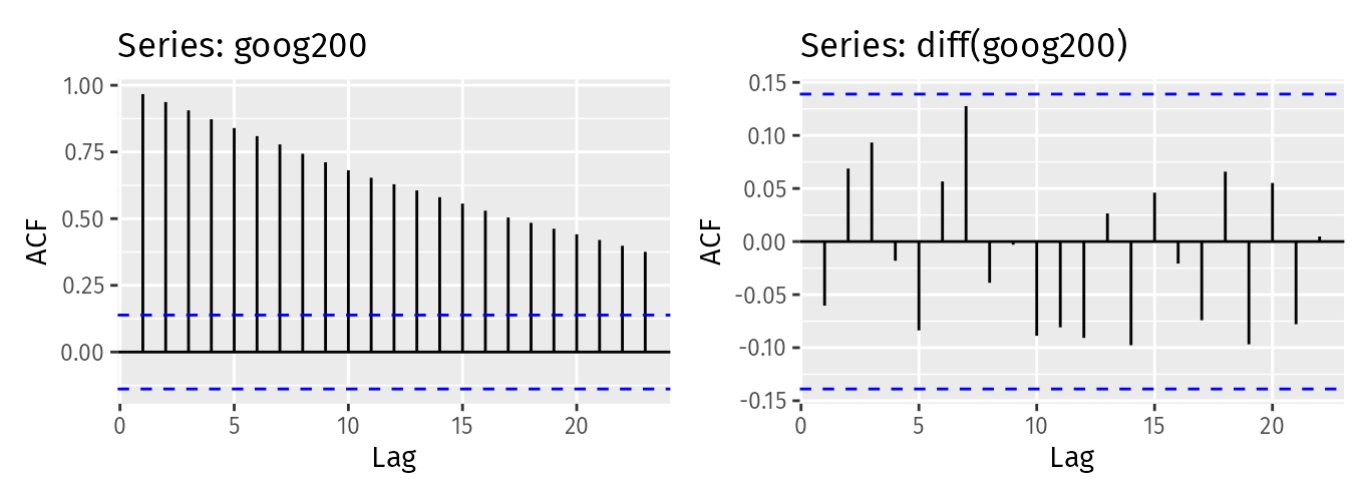
\includegraphics[scale=0.25]{img/acf}
		\caption{Gráfico ACF: no estacionario (izquierda) vs estacionario (derecha) \cite{hyndman2021stationarity}}
		\label{acf}
	\end{figure}  	
	
	Numéricamente, la autocorrelación en un retardo \( k \) equivale a:
	
	\[
	\rho_k = \frac{\mathrm{Cov}(y_t, y_{t-k})}{\sigma^2}
	\]
	
	donde \( \sigma^2 \) es la varianza de la serie y \( \mathrm{Cov}(y_t, y_{t-k}) \) es la covarianza entre los valores actuales y los desplazados \( k \) periodos atrás.
	
	
	\item El test ADF, por su parte, nos proporciona la misma conclusión de manera numérica, para lograr un mayor rigor estadístico en la solución. Su funcionamiento radica en la búsqueda de una raíz unitaria en la serie, en cuyo caso significa que la serie presenta comportamiento no estacionario.
	
	De forma general, el test se basa en ajustar una regresión del tipo:
	
	\[
	\Delta y_t = \alpha + \beta t + \gamma y_{t-1} + \sum_{i=1}^{p} \delta_i \Delta y_{t-i} + \epsilon_t
	\]
	
	donde \( \Delta y_t = y_t - y_{t-1} \) representa la primera diferencia de la serie, \( \gamma \) es el parámetro clave para detectar la raíz unitaria, y \( \epsilon_t \) es el error.
	
	Sin embargo, lo más relevante para su uso es comprender cómo funciona el test de hipótesis. Como hipótesis nula (\( H_0 \)), define que la serie no es estacionaria, es decir, que presenta una raíz unitaria, y como (\( H_1 \)) podremos aceptar que la serie sea estacionaria. Para ello, basta con observar el valor de p:
	
	\begin{itemize}
		\item Si el \textbf{p-valor} del test es significativo se puede rechazar la hipótesis nula. En ese caso, la serie puede considerarse estacionaria, y podemos parar el proceso iterativo de diferenciación.
		\item Si el \textbf{p-valor} es mayor al valor de significación, no podemos rechazar la hipótesis nula, lo que indica que la serie sigue siendo no estacionaria, y debemos continuar el proceso de integración.
	\end{itemize}
	
\end{itemize}


\paragraph{Componente autoregresiva (AR)}


Esta parte del modelo representa la relación entre el valor actual de la serie y sus valores pasados. Supone que el valor presente puede explicarse como una combinación lineal de observaciones anteriores, los cuales se denominan retardos o lags. Normalmente, el número de lags a emplear es un hiperparámetro clave del modelo, el cual es controlado por  \( p \).

	Matemáticamente, podemos expresarlo como:
	
	\[
	z_t = w_1 y_{t-1} + w_2 y_{t-2} + \cdots + wi_p y_{t-p} + \varepsilon_t
	\]
	
	donde:
	\begin{itemize}
		\item \( w_1, w_2, \ldots, w_p \) son los coeficientes autoregresivos que indican el peso o importancia de cada valor pasado. Cuando usamos el valor p, establecemos el número de valores con peso 1 que tomará nuestro modelo, mientras que el resto se mantienen a 0.  Pero, podríamos tener variantes en las que dichos pesos fueran valores flotantes entre 0 y 1 que permitan una ponderación más refinada de los valores.
		\item \( \varepsilon_t \) es el término asociado al error en el instante \( t \).
	\end{itemize}
	
	Gracias a la componente AR, podemos capturar relaciones de corto plazo y patrones de dependencia temporal, siempre que la serie sea estacionaria. Es habitual que muchas series temporales muestren este tipo de estructura, donde los valores pasados son predictivos del comportamiento futuro inmediato, como ya vimos con el caso de las temperaturas y el consumo eléctrico. Por tanto, la elección del parámetro \( p \) es clave:  un valor pequeño implica que sólo los valores más recientes tengan influencia, mientras que un valor mayor permite capturar relaciones más amplias en el tiempo, pero puede aumentar el riesgo de sobreajuste y se pierda localidad. En definitiva, se trata de un elemento esencial del rendimiento de ARIMA, por lo que es clave elegir adecuadamente su valor.
	
	\paragraph{Componente de media móvil (MA)}
	
	
	Por último, nos queda describir el funcionamiento de la media móvil. Esta tiene como objetivo modelar la parte estocástica de la serie temporal, es decir, los errores de predicción cometidos en instantes anteriores. Anteriormente,  vimos que la parte autoregresiva se basaba en realizar la media sobre sus mismos valores, mientras que aquí tratamos de extraer información de los residuos.
	
	Formalmente, un modelo MA de orden \( q \) se define como:
	
	\[
	y_t = \mu + \varepsilon_t + \theta_1 \varepsilon_{t-1} + \theta_2 \varepsilon_{t-2} + \cdots + \theta_q \varepsilon_{t-q}
	\]
	
	donde:
	\begin{itemize}
		\item \( y_t \) es el valor observado de la serie en el instante \( t \),
		\item \( \mu \) es la media de la serie (si está centrada, puede ser cero),
		\item \( \varepsilon_t \) es el término de error en el instante \( t \),
		\item \( \theta_1, \ldots, \theta_q \) son los coeficientes del modelo MA.
	\end{itemize}
	
	Esto nos permitirá capturar patrones aleatorios que no pueden explicarse mediante una simple tendencia o correlación temporal, y por tanto, mejorando los resultados y el rendimiento del modelo, al suavizarse los errores pasados para acercanos más a la serie real. Por tanto, el número de errores a considerar \textit{q} debe escoger de manera adecuada. Para facilitar esta decisión, podemos basarnos de nuevo en dos enfoques: en emplear la información del gráfico ACF, o bien, de manera experimental:
	
	\begin{itemize}
		\item El análisis gráfico mediante ACF nos permite analizar el comportamiento de los lags; en un modelo MA puro, los primeros \( q \) retardos (\textit{lags}) suelen mostrar autocorrelación significativa, pero luego suelen decrecer de manera repentina a cero. Una buena estimación puede ser tomar como valor de \( q \)  el último lag con autocorrelación significativa antes del corte. Es decir, si a partir del punto q+1 se produce un descenso abrupto, tomamos \textit{q}.
		
		\item Si la gráfica no nos proporciona una respuesta clara, y la serie es modelable en un tiempo razonable, se puede realizar una búsqueda hiperparámetros, probando diferentes valores de \( q \), y entrenando un modelo ARIMA para cada combinación posible (junto a valores de \( p \) y \( d \)), y evaluar su rendimiento utilizando métricas como el \textit{Mean Squared Error} (MSE). Para facilitar el proceso, podemos usar técnicas clásicas como grid search, que no es más que realizar todas las combinaciones posibles de parámetros p,q y d. Pero, de manera más avanzada, existen adaptaciones de ARIMA en frameworks como auto\_arima,  que usan una estimación automática de los hiperparámetros.
	\end{itemize}
	

\paragraph{Conclusiones}


En resumen, ARIMA nos permite modelar gran cantidad de problemas de manera simple, cumplendo como única restricción la estacionariedad. Pero principalmente esta característica, si bien facilita enormemente el proceso, también impacta sobre la calidad del resultado; si la serie tiene una estructura muy compleja y no estacionaria, convertirla para que lo sea puede provocar una pérdida masiva de información, ya que al diferenciar estamos suprimiendo información que podría ser potencialmente relevante. En casos extremos, la pérdida de expresividad podría ser tal hasta lograr una serie muy plana, sin comportamientos aparentes. Por tanto, es necesario emplear técnicas más sofisticadas que no requieran dicha condición para extraer modelos más generalizables.\\

Por otro lado, las predicciones a largo plazo también son problemáticas: como se buscan relaciones lineales entre variables, con estaciones definidas, y variables sencillas de representar, cuando se usa ante series complejas puede tenderse a formular una predicción bastante plana y poco informativa que tienda a la media, ante la imposibilidad del modelo a adaptarse a los cambios. De manera directa, esto influencia también ante la capacidad de adaptación de los outliers: ante su presencia, se podría ver alterada la predicción real, y se deben estudiar y analizar en fases previas de preprocesado.\\

Por último, en caso de que se disponga de información adicional, como intervalos de tiempo, localización en calendario, habitualmente usada cuando se dispone de datos de larga extensión para facilitar su estructuración y la detección de períodos, no es posible incorporarlo de forma directa. Habría que realizar modificaciones sobre este, como por ejemplo, las integradas en ARIMAX, que se basa en la implementación original \cite{box1970time}, pero añadiendo de manera aditiva operaciones adicionales aprovechando la información externa.

\subsubsection{Prophet}

Como alternativa más reciente de los modelos aditivos, disponemos de Prophet \cite{taylor2018prophet}. Desarrollado por Meta, apareció teniendo como objetivo facilitar la generación de predicciones de calidad, incluso si es empleado por analistas sin experiencia en series temporales. Según su blog oficial \cite{prophet2017}, Prophet fue creado para responder a la necesidad de escalar la producción de pronósticos precisos en entornos empresariales sin necesidad de altos conocimientos para poder extraer buenas conclusiones. 

\paragraph{Funcionamiento}


A diferencia de los modelos anteriores, que definían la necesidad de cumplir ciertas restricciones, como la estacionariedad, Prophet nos permite trabajar con entornos más cambiantes, al estar diseñado para recibir datos de al menos varios meses de duración, donde si bien existen patrones estacionales claros por la estructura de tipo calendario, es capaz de adaptarse a cambios e imprevistos. Es decir, es capaz de modelar días festivos o de caracter especial sobre el impacto del desarrollo de la serie (como el lanzamiento de un nuevo servicio o producto de una empresa) y es más robusto frente a outliers que los modelos que vimos anteriormente. (ver figura \ref{prophetex}).\\

La descomposición se basa en una suma de tres componentes, de manera similar a los modelos anteriores:

\begin{equation}
	y(t) = g(t) + s(t) + h(t) + \varepsilon_t
\end{equation}

Donde:

\begin{itemize}
	\item \( g(t) \) representa la {tendencia a largo plazo}, que puede ser lineal o logística, y puede contener cambios de tendencia que se ajustan de manera automática.
	\item \( s(t) \) modela la {estacionalidad} periódica mediante funciones basadas en series de Fourier. Permite capturar estacionalidades diarias, semanales o anuales, aunque las implementaciones disponibles permiten también especificar intervalos definidos por el usuario.
	\item \( h(t) \) representa efectos de festividades o eventos especiales, introducidos manualmente por el usuario.
	\item \( \varepsilon_t \) representa el error asociado a la predicción realizada, que se asume con distribución normal.
\end{itemize}

Entrando en mayores detalles de implementación, una de las principales novedades reside en algo tan sencillo de visualizar como la tendencia. Hasta ahora, normalmente disponíamos de un modelado de única ecuación, comúnmente lineal, que era común a toda la serie. Pero Prophet es más flexible gracias a la detección automática de cambios de pendiente, los cuales denomina \textit{changepoints}. Además, para reflejar comportamientos y cambios de tendencia de manera más suave y progresiva, permite ajustar la suavidad en torno a los changepoints mediante un parámetro de escala.

\begin{figure}[H] %con el [H] le obligamos a situar aquí la figura
	\centering
	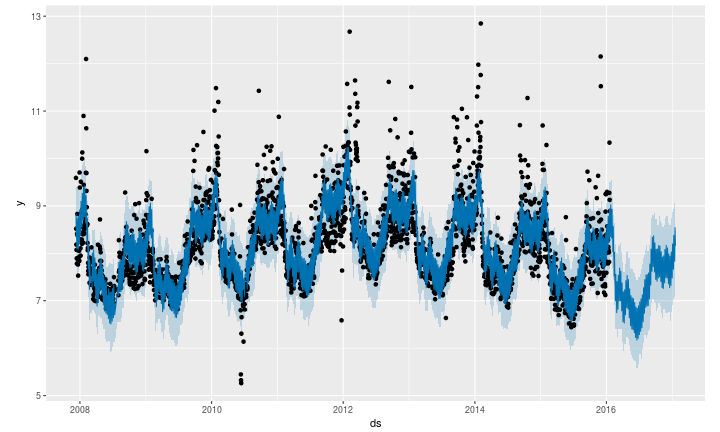
\includegraphics[scale=0.375]{img/prophetex}
	\caption{Prophet: Ejemplo de predicción en entorno ruidoso  \cite{prophet2017}}
	\label{prophetex}
\end{figure}  	


Adicionalmente, la modelización de la estacionalidad también recibe un formulación más sofisticada. Usando Fourier, podemos introducir la duración del período de cada ciclo (\textit{P}) e ir ajustando su precisión mediante el parámetro \textit{n} (ver ecuación \ref{fftprophet}). Pero lo más interesante es que se facilita la inclusión explícita de festividades o eventos que pueden afectar significativamente la serie. Para ello, el modelo permite especificar ventanas alrededor de esos puntos para así aprender también su comportamiento.

\begin{equation}
	s(t) = \sum_{n=1}^{N} \left[ a_n \cos\left( \frac{2\pi n t}{P} \right) + b_n \sin\left( \frac{2\pi n t}{P} \right) \right]
	\label{fftprophet}
\end{equation}

\paragraph{Conclusiones}

En resumen, Prophet supone un salto considerable en cuanto a adaptación y cercanía a los datos extraídos de casos reales. Nos permite insertar la información explícita que mencionabamos en ARIMA, ya que nos permite añadir de manera muy intuitiva información adicional del problema. Además, en su publicación original se destaca la eficacia incluso cuando los datos presentan imperfecciones, como valores atípicos, datos faltantes o cambios abruptos en la tendencia, lo cual facilita enormemente el proceso de preprocesado, el cual puede reducirse al mínimo. Esto aporta considerablemente a su faceta relacionada con la facilidad de uso.\\

Sin embargo, aunque supone un gran salto con lo disponible anteriormente, aún se siguen manteniendo varias de las limitaciones que venimos analizando a lo largo de los modelos. En primer lugar, podemos observar que su enfoque podría verse más implicado en el ajuste de curvas que en una modelación como tal de las dependencias temporales, que nos permitan realizar forecasting a largo plazo. Si bien el modelo destaca por su sencillez al usuario, la elección de parámetros sigue siendo un aspecto delicado, ya que el modelo puede incurrir en sobreajuste si no se calibran adecuadamente. Debemos asegurarnos de sus valores estudiando previamente el conjunto de datos.\\

 Finalmente, Prophet no incluye de manera nativa mecanismos autoregresivos ni permite modelar series multivariantes, lo cual representa una limitación cuando trabajamos con series que miden varios factores al mismo tiempo, y que incluso pueden estar correlacionados entre sí.

\subsubsection{Comparativa final y limitaciones}

A lo largo de este apartado, hemos analizado tres de los enfoques más relevantes para la descomposición de series temporales: {STL}, {ARIMA} y {Prophet}. Aunque todos comparten el mismo objetivo, que es separar la serie en componentes interpretables como tendencia, estacionalidad y ruido, cada uno lo aborda desde una perspectiva distinta, lo que se traduce en ventajas e inconvenientes específicos (ver tabla \ref{tab:modelsadit}).

\begin{itemize}


\item El método \textbf{STL} nos ha resultado especialmente útil en las fases de análisis exploratorio. Su uso de suavizado local mediante Loess le permite adaptarse a estacionalidades no necesariamente fijas y proporciona una descomposición visualmente clara e interpretable. Sin embargo, al tratarse de un enfoque puramente descriptivo, su utilidad para la predicción es limitada, y se requieren herramientas adicionales.

\item Por su parte, \textbf{ARIMA} representa una aproximación estadística clásica basada en la modelización de las diferentes componentes temporales de la serie. Hemos establecido que resulta eficaz en series estacionarias con comportamientos lineales, gracias a su capacidad para capturar tanto relaciones autoregresivas como de medias móviles.  Pero la necesidad de afinar los hiperparámetros, la precondición de estacionareidad y su naturaleza lineal limita su rendimiento ante patrones no lineales o estacionalidades más complejas.

\item Por último, \textbf{Prophet} es una solución más moderna y accesible, especialmente diseñada para aplicaciones empresariales. A diferencia de ARIMA, no exige estacionariedad y su estructura facilita su uso por usuarios sin conocimientos especiales sobre series temporales. Sin embargo, carece de componentes autoregresivos y no modela relaciones multivariantes de forma nativa, lo que puede comprometer su versatilidad.

\end{itemize}

\begin{table}[H]
	\centering
	\begingroup
	\renewcommand{\arraystretch}{1.055}
	\begin{tabular}{P{3.3cm} | P{2.5cm} P{2.5cm} P{2.5cm}}
		\toprule
		\textbf{Característica} & \textbf{STL} & \textbf{ARIMA} & \textbf{Prophet} \\
		\midrule
		Enfoque & Suavizado Loess & Modelo estadístico autoregresivo & Modelo aditivo estructurado \\
		Requiere estacionariedad & No & Sí & No \\
		Componente de tendencia & Suavizado local & Parte del modelo (AR/I) & Curva lineal o logística con puntos de cambio \\
		Modelado de estacionalidad & Suavizado periódico & Diferenciación estacional o SARIMA & Series de Fourier \\
		Eventos especiales & No contemplado & No los contempla & Incluidos explícitamente \\
		Capacidad predictiva & Limitada & Buena si la serie es estacionaria y lineal & Alta en escenarios empresariales comunes \\
		Robustez ante valores atípicos & Alta & Baja & Alta \\
		Facilidad de uso & Media & Baja & Alta \\
		Interpretabilidad & Muy alta & Media & Muy alta \\
		\bottomrule
	\end{tabular}
	\caption{Comparativa entre métodos de descomposición de series temporales}
	\label{tab:modelsadit}
	\endgroup
\end{table}



En resumen, podemos afirmar que estos modelos constituyen una base sólida para el análisis inicial de series temporales, pero enfrentamos varias dificultades con datos dinámicos, dependencias de largo plazo, series multivariantes o patrones no lineales. Es en estos contextos donde se vuelve necesaria la incorporación de modelos más avanzados, como las {redes neuronales recurrentes (RNN)} o incluso los {Transformers}, que permiten modelar dependencias temporales profundas de manera eficiente y escalar a volúmenes de datos mayores. En los apartados siguientes, analizaremos estos nuevos modelos.

\subsection{Redes Neuronales Recurrentes}

Hasta ahora, la mayoría de soluciones estudiadas se han basado en el procesamiento de un conjunto de datos de entrada, que es procesado y modelado de manera más o menos sofisticada, y se otorga una salida, como, por ejemplo, los modelos de descomposición que hemos abordado hasta ahora. No obstante, en escenarios donde las series temporales presentan relaciones no lineales complejas, múltiples escalas de dependencia y estructuras difíciles de modelar de forma explícita, resulta necesario recurrir a modelos más avanzados.\\

Podríamos pensar en emplear modelos tradicionales vistos en otros ámbitos, como las redes neuronales. Pero en dichos problemas, las entradas y salidas no guardan una relación entre sí; son independientes. En los conjuntos de entrenamiento habituales, como problemas tabulares de regresión o clasificación, lo que nos importa es asignar el valor adecuado, y normalmente, cada instancia es independiente del resto. Pero cuando disponemos de información secuencial, como el lenguaje natural, o en nuestro caso, las series temporales, esto no es así.\\

 En los métodos basados en descomposición, hemos podido apreciar que nos basamos continuamente en los valores pasados para ser capaces de modelar perdiendo la mínima información posible, y que por ejemplo, encontrar patrones como la estacionalidad es de gran importancia para minimizar el error y a su vez simplificar el modelado. Esto descarta la utilización de perceptrones multicapa, o capas densamente conectadas para el modelado de series temporales con un mínimo de complejidad, debido a dicha dependencia. Solo quizás, podríamos modelar series simples con una clara tendencia y forma, debido a que podrían asemejarse a una regresión. Pero si queremos obtener resultados escalables a redes más compleja, debemos tener en cuenta las conexiones temporales entre cada timestamp, y modelar dicho orden dentro de la secuencia global de los datos. Esto lo podemos conseguir relacionando cada salida con la anterior y es así como surge el concepto de las Redes Neuronales Recurrentes.
 
 \subsubsection{Funcionamiento de las RNN}
 
 Las RNN, al igual que las redes neuronales tradicionales, son capaces de procesar una entrada y arrojar una salida, modelando los datos internamente mediante sus capas ocultas. Pero la diferencia radica en la necesidad de establecer conexiones entre la salida anterior y la entrada actual. Esto se consigue con conexiones recurrentes que permiten que la información fluya de un instante al siguiente dentro de la propia red (ver figura \ref{rnn}).
 
 \begin{figure}[H] %con el [H] le obligamos a situar aquí la figura
 	\centering
 	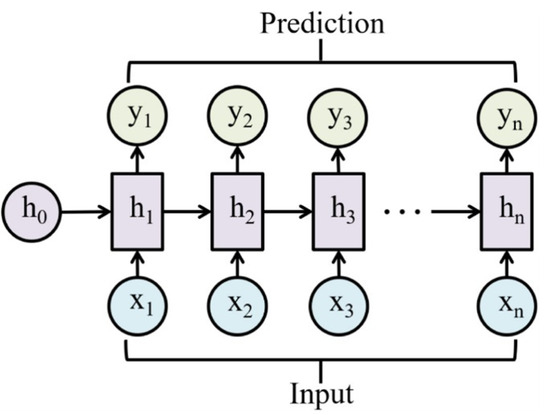
\includegraphics[scale=0.4]{img/rnn}
 	\caption{RNN: arquitectura del modelo \cite{info15090517}}
 	\label{rnn}
 \end{figure}  	
 
Estructuralmente, una RNN clásica está compuesta de tres capas principales \cite{info15090517}: una capa de entrada, una capa oculta con conexiones recurrentes, y una capa de salida. El comportamiento de la red se define en función de cómo se actualiza su estado interno y cómo se generan las salidas. En su definición original, en cada instante de tiempo \( t \), la red recibe un vector de entrada \( \mathbf{x}_t \) y actualiza su estado oculto \( \mathbf{h}_t \) según la siguiente ecuación:

\begin{equation}
	\mathbf{h}_t = \sigma_h(\mathbf{W}_{xh} \mathbf{x}_t + \mathbf{W}_{hh} \mathbf{h}_{t-1} + \mathbf{b}_h)
\end{equation}

donde:
\begin{itemize}
	\item \( \mathbf{W}_{xh} \) es la matriz de pesos entre la entrada y la capa oculta,
	\item \( \mathbf{W}_{hh} \) representa la conexión recurrente entre los estados ocultos,
	\item \( \mathbf{b}_h \) es el vector de sesgo asociado,
	\item \textbf{\( \sigma_h \)} es la función de activación, normalmente la tangente hiperbólica (\texttt{tanh}) o la rectificada lineal (\texttt{ReLU}).
\end{itemize}

A partir del estado oculto actualizado, se calcula la salida correspondiente mediante:

\begin{equation}
	\mathbf{y}_t = \sigma_y(\mathbf{W}_{hy} \mathbf{h}_t + \mathbf{b}_y)
\end{equation}

donde:
\begin{itemize}
	\item \( \mathbf{W}_{hy} \) conecta la capa oculta con la capa de salida,
	\item \( \mathbf{b}_y \) es el vector de sesgo en la salida,
	\item \textbf{\( \sigma_y \)} es la función de activación de la salida.
\end{itemize}

Gracias principalmente al estado oculto, podemos integrar la información de entrada actual con las salidas previas, permitiendo que la red exhiba un comportamiento ordenado temporalmente en sus salidas. Pero, sin lugar a dudas, otro de los elementos clave para el funcionamiento adecuado es escoger una correcta función de activación \( \sigma_h \), ya que se encarga de añadir la no linearidad a la salida. Una de las más empleadas es la tangente hiperbólica, $tanh$, que permite ajustar los valores de los pesos al intervalo [-1,1], el cual es bastante intuitivo gracias al estar centrado en cero, y además, permite la existencia de pesos tanto positivos como negativos.

\begin{equation}
	\tanh(x) = \frac{e^x - e^{-x}}{e^x + e^{-x}}
\end{equation}
  
 También es posible encontrar ReLU o sus variantes, ya que permiten ajustar los pesos de manera computacionalmente sencilla, pero solo permite el paso de valores positivos. 
 
 \begin{equation}
 	ReLU(x) = max(0, x)
 	\label{eq:relu}
 \end{equation}

Elegir una u otra opción depende del tipo de problema que tratemos de resolver o incluso del conjunto de datos de entrada, pero es un elemento clave que afecta directamente al aprendizaje de los estados ocultos y la propagación de dicha información.

\subsubsection{Limitaciones de las RNN estándar}

Aunque las RNN suponen un gran avance en el aprendizaje de datos secuenciales y permitieron una mejora considerable en los resultados, no están exentas de problemas durante el aprendizaje. Al igual que otros modelos que usan la propagación mediante gradientes, debemos tener especial cuidado con su gestión para evitar la explosión de gradientes y, en su caso, el extremo contrario, el desvanecimiento.\\

Estos efectos se ven potenciados debido al particular funcionamiento del algoritmo de retropropagación entre los diferentes pasos temporales. A diferencia de una red neuronal clásica, necesitamos que los pesos tengan relación también con los pasos anteriores de la secuencia, y para lograrlo, debemos modificar el proceso, de manera que podamos emplear el procedimiento habitual con la nueva estructura oculta de pesos. En cada etapa de actualización:

\begin{enumerate}
	\item La RNN se desenrolla (\textit{unroll}) en el tiempo durante un número finito de pasos (por ejemplo, 10).
	
	\item Se aplica retropropagación en la red desenrollada de la manera habitual.
	
	\item Se acumulan los gradientes de todos los pasos temporales hacia los pesos compartidos.
	
	\item Los parámetros se actualizan con una optimización como SGD o Adam.
\end{enumerate}

De esta forma, implementamos el mecanismo conocido como \textit{Backpropagation Through Time} (BPTT). Durante el entrenamiento con este mecanismo, calculamos los gradientes de la función de pérdida respecto a los pesos de la red a lo largo de varios pasos temporales, y es al propagar cuando podemos enfrentarnos a los dos problemas ya mencionados: la explosión y el desvanecimiento del gradiente.\\

El desvanecimiento del gradiente se produce si los términos derivados que aparecen en el cálculo (concretamente, los productos sucesivos de matrices Jacobianas) tienen valores propios menores que uno, su multiplicación sucesiva tiende a cero. Esto provoca que los gradientes disminuyan exponencialmente a medida que retrocedemos en el tiempo, impidiendo que la red actualice adecuadamente los pesos de las capas o pasos más antiguos, y como consecuencia, la red pierde la capacidad de aprender dependencias a largo plazo, ya que el error no alcanza a modificar significativamente las entradas lejanas.\\
	
Por otro lado, la explosión del gradiente es justo el caso opuesto; si los valores propios de las Jacobianas son mayores que uno, la multiplicación produce gradientes que crecen exponencialmente. Esto puede llevar a actualizaciones de pesos excesivas, provocando inestabilidad numérica. En ambos casos, por tanto, la capacidad de aprendizaje de la red se ve comprometida, y puede perjudicar gravemente a los resultados obtenidos.\\

Formalmente, podemos ver reflejado este comportamiento mediante el desarrollo de los estados ocultos. A partir de la fórmula recurrente del estado oculto:

\begin{equation}
	\mathbf{h}_t = \sigma_h\left( \mathbf{W}_{xh} \mathbf{x}_t + \mathbf{W}_{hh} \, \sigma_h\left( \mathbf{W}_{xh} \mathbf{x}_{t-1} + \mathbf{W}_{hh} \mathbf{h}_{t-2} + \mathbf{b}_h \right) + \mathbf{b}_h \right),
	\label{eq:hidden_state_expansion}
\end{equation}

el cálculo del gradiente de \(\mathbf{h}_t\) respecto a un estado anterior \(\mathbf{h}_{t-n}\) implica el producto de Jacobianas:

\begin{equation}
	\frac{\partial \mathbf{h}_t}{\partial \mathbf{h}_{t-n}} = \prod_{k=t-n}^{t-1} \mathbf{J}_k,
	\label{eq:jacobian_product}
\end{equation}

donde \(\mathbf{J}_k\) representa la matriz Jacobiana del estado oculto en el instante \(k\). La estabilidad de estos productos depende críticamente de los valores propios de \(\mathbf{J}_k\), por lo que se trata del elemento clave causante de las dos problemáticas descritas.\\

Para tratar de solucionar este problema, podemos encontrar variantes de este algoritmo en el estado del arte. Algunas, tratan de simplemente modificar el funcionamiento de la propagación, con técnicas como el \textit{gradient clipping}, que permiten limitar el tamaño máximo del gradiente durante la retropropagación, evitando explosiones incontroladas. Pero también podemos encontrar arquitecturas específicas como las LSTM (Long Short-Term Memory), que introducen mecanismos de control del flujo de información mediante puertas, facilitando la retención de información relevante a largo plazo y mitigando el problema desvanecimiento de gradientes de manera estructural.

\subsubsection{LSTM}

Para resolver los problemas de desvanecimiento del gradiente asociados a las RNN clásicas, Hochreiter y Schmidhuber propusieron en 1997 las \textit{Long Short-Term Memory networks} (LSTM)~\cite{10.1162/neco.1997.9.8.1735}. La innovación clave de estas redes es la introducción de mecanismos de puertas que regulan el flujo de información a lo largo del tiempo, permitiendo mantener una memoria a largo plazo de forma más estable.\\

Cada célula LSTM incorpora tres compuertas principales: la compuerta de entrada, la compuerta de olvido y la compuerta de salida. Estas compuertas permiten decidir qué información se debe incorporar, qué parte del estado anterior se debe olvidar y qué parte del nuevo estado se debe transmitir a la siguiente etapa. Gracias a este diseño, las redes LSTM son especialmente eficaces para modelar dependencias temporales de largo alcance.

El comportamiento interno de una célula LSTM se puede describir mediante las siguientes ecuaciones:

\begin{align}
	i_t &= \sigma(W_{xi}x_t + W_{hi}h_{t-1} + b_i) \quad &\text{(compuerta de entrada)} \\
	f_t &= \sigma(W_{xf}x_t + W_{hf}h_{t-1} + b_f) \quad &\text{(compuerta de olvido)} \\
	o_t &= \sigma(W_{xo}x_t + W_{ho}h_{t-1} + b_o) \quad &\text{(compuerta de salida)} \\
	g_t &= \tanh(W_{xc}x_t + W_{hc}h_{t-1} + b_c) \quad &\text{(nuevo contenido candidato)} \\
	c_t &= f_t \odot c_{t-1} + i_t \odot \tilde{c}_t \quad &\text{(estado de la celda)} \\
	h_t &= o_t \odot \tanh(c_t) \quad &\text{(estado oculto)}
\end{align}

Donde $\sigma$ representa la función sigmoide, $\tanh$ la tangente hiperbólica, y $\odot$ la multiplicación elemento a elemento. Esta arquitectura permite mantener y actualizar información relevante a lo largo del tiempo, mitigando los problemas habituales en el aprendizaje de secuencias largas.\\

Cada compuerta dentro de una celda LSTM desempeña una función específica en la regulación del flujo de información. La compuerta de entrada controla cuánta información del nuevo vector de entrada $x_t$ se incorpora al estado de la celda $c_t$; la compuerta de olvido determina qué parte del estado anterior $c_{t-1}$ se retiene, y, finalmente, la compuerta de salida decide cuánta información del estado actual $c_t$ se utiliza para calcular el estado oculto $h_t$ (ver figura \ref{lstm}).

\begin{figure}[H] %con el [H] le obligamos a situar aquí la figura
	\centering
	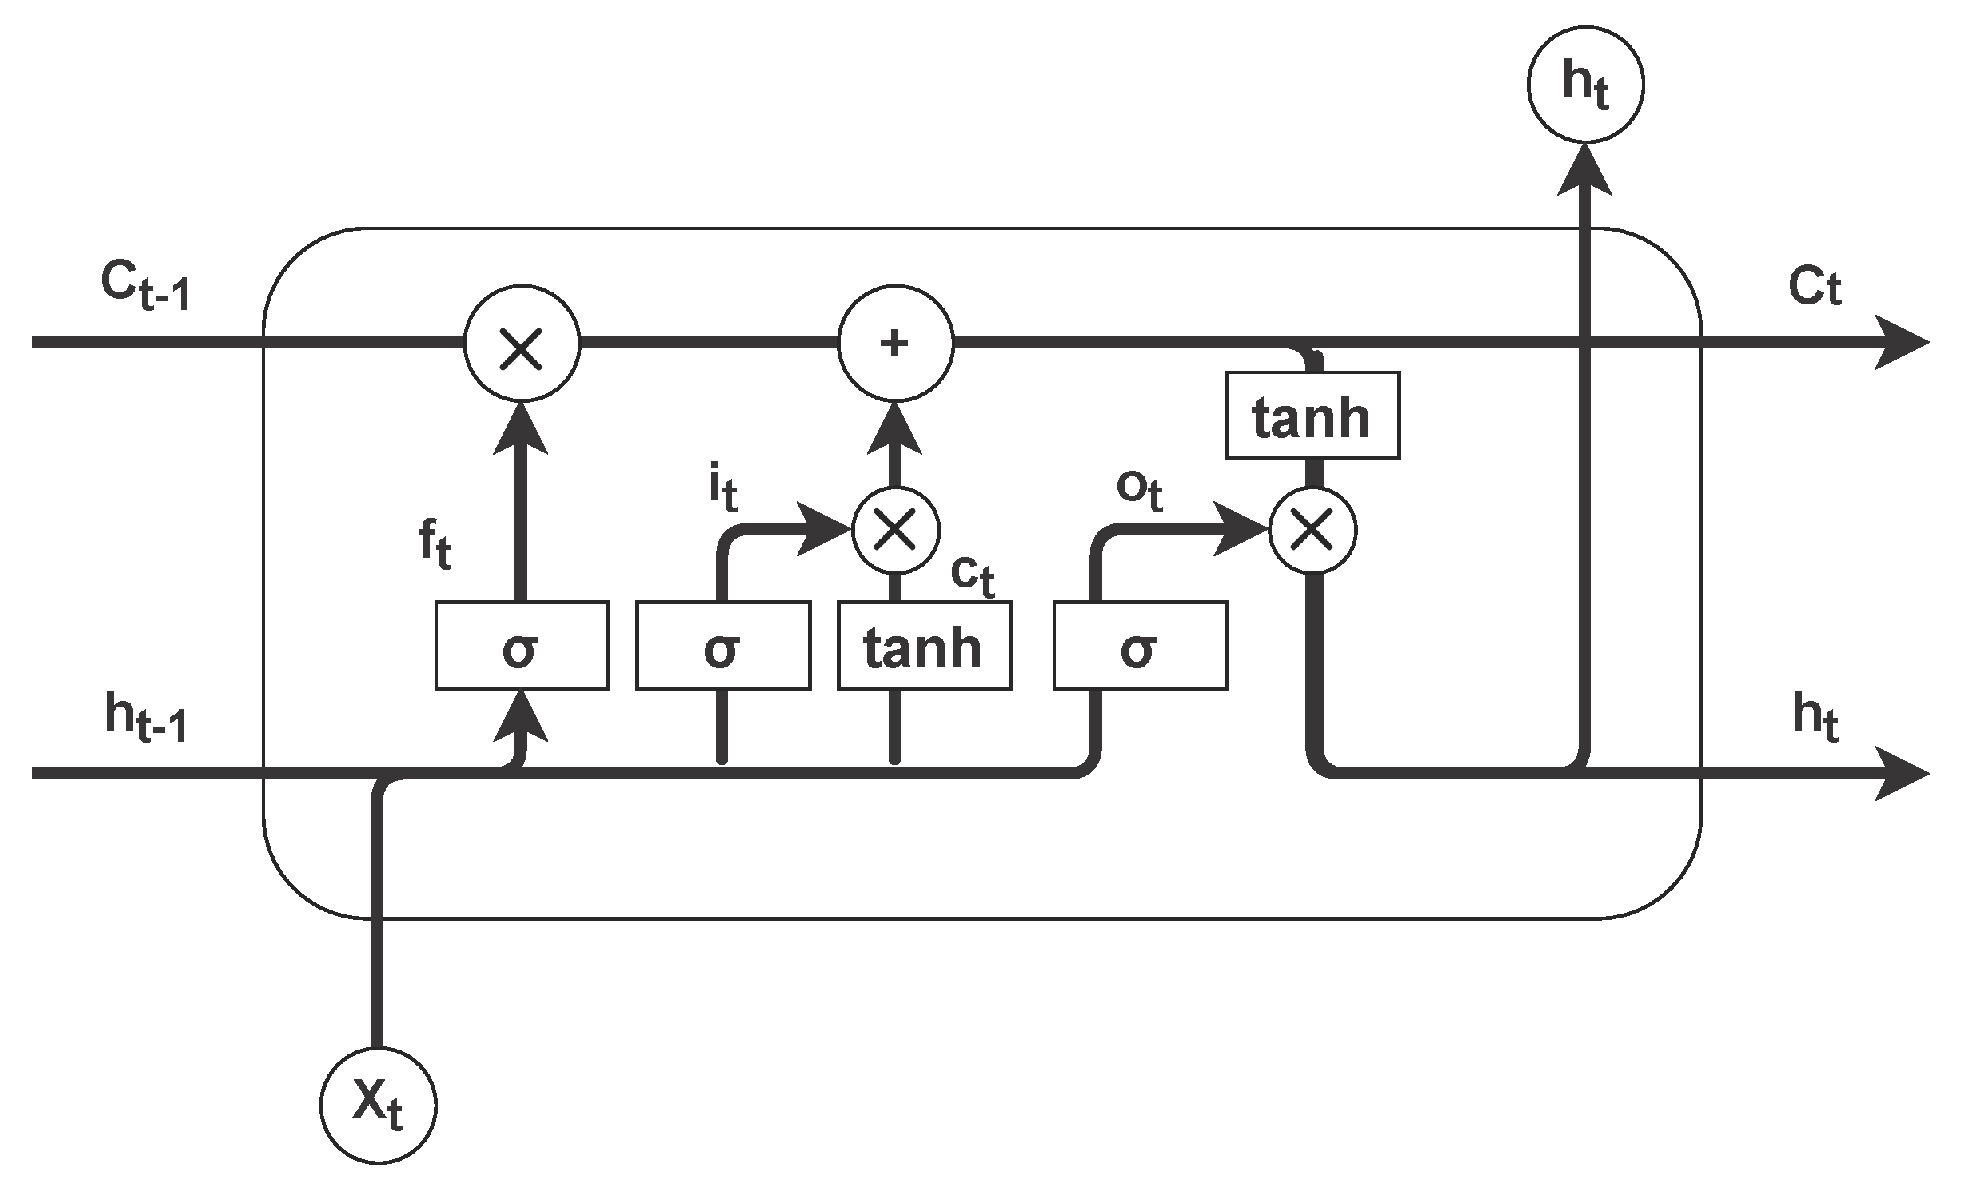
\includegraphics[scale=1]{img/lstm}
	\caption{LSTM: funcionamiento de la arquitectura de puertas}
	\label{lstm}
\end{figure}  	


Además, la entrada candidata de la celda, denotada como $g_t$, representa nueva información que podría añadirse al estado de la celda tras ser modulada por la compuerta de entrada.\\

Gracias a estos mecanismos de control, las redes LSTM pueden decidir dinámicamente qué información conservar o descartar en cada momento, lo que les permite gestionar dependencias temporales a largo plazo de manera mucho más eficaz que las RNN convencionales. La recurrencia se mantiene a través del estado de la celda $c_t$, que permite el traspaso continuo de información entre pasos temporales. Este flujo sostenido de memoria facilita la conservación de patrones relevantes a lo largo de secuencias de larga extensión. Por otro lado, las multiplicaciones elemento a elemento entre compuertas y vectores asociados aseguran una interacción eficiente entre componentes y posibilitan transformaciones complejas sin comprometer la estabilidad durante el entrenamiento. En conjunto, gracias a todos estos elementos, las LSTM mantienen un equilibrio entre flexibilidad, memoria y estabilidad en el aprendizaje.\\

Sin embargo, no suponen la solución definitiva a los problemas, pues, si bien conseguimos solucionar el problema de los gradientes, hemos incorporado complejidad adicional al modelo que puede afectar en diferentes aspectos:

\begin{itemize}
	\item \textbf{Complejidad computacional:} se requieren más recursos que modelos más simples debido al uso de múltiples compuertas y operaciones por paso temporal, incrementando el número de parámetros y el tiempo de entrenamiento. Además, su estructura recurrente impide aprovechar eficientemente las GPU, y aprovechar su potencia para lograr un buen escalado.
	
	\item \textbf{Dificultad para capturar dependencias muy largas:} Aunque superan a las RNN básicas, si tratamos de modelar predicciones a largo plazo, como buscamos en este trabajo, podemos apreciar una pérdida de efectividad.
	
	\item \textbf{Sensibilidad a la configuración:} el rendimiento depende de manera sensible de los parámetros escogidos, cuya selección no es una tarea trivial y puede afectar considerablemente a los resultados.
	
	\item \textbf{Interpretabilidad:} aunque su arquitectura muestra el flujo que sigue la información, interpretar de forma precisa el funcionamiento interno es un proceso complicado al agregar elementos adicionales como las puertas.

\end{itemize}

A modo de conclusión, aunque las LSTM representaron un avance fundamental en el ámbito del forecasting, en aplicaciones modernas suelen ser superadas por arquitecturas más flexibles y escalables como los Transformers, los cuales estudiaremos a continuación, y serán nuestro principal foco de atención.

\section{Transformers}

Los Transformes son una de las mayores invenciones de los últimos años en el tratamiento de datos secuenciales, como el lenguaje natural, y en series temporales. Su estructura (ver figura \ref{trans}), la cual propone el uso de mecanismos basados en atención, ha permitido prescindir de los algoritmos basados en recurrencia, y simplificar el proceso complejo de aprendizaje que teníamos debido a los problemas con la propagación y los gradientes.\\

A diferencia de las redes RNN o LSTM, que procesan la información de forma secuencial y requieren mantener estados ocultos a lo largo del tiempo, los Transformers permiten procesar todas las posiciones de la secuencia en paralelo, lo que mejora drásticamente la eficiencia computacional y la capacidad de modelar relaciones a largo plazo. Esto nos permite también aprovechar arquitecturas de computación con gran capacidad para la paralelización, como el uso de GPUs, y así reducir tiempos de ejecución, o bien, aprovechar la capacidad extra de paralelización para enfrentarnos a problemas mucho más complejos, con mayor número de parámetros y dependencias a largo plazo.

\begin{figure}[!ht] %con el [H] le obligamos a situar aquí la figura
	\centering
	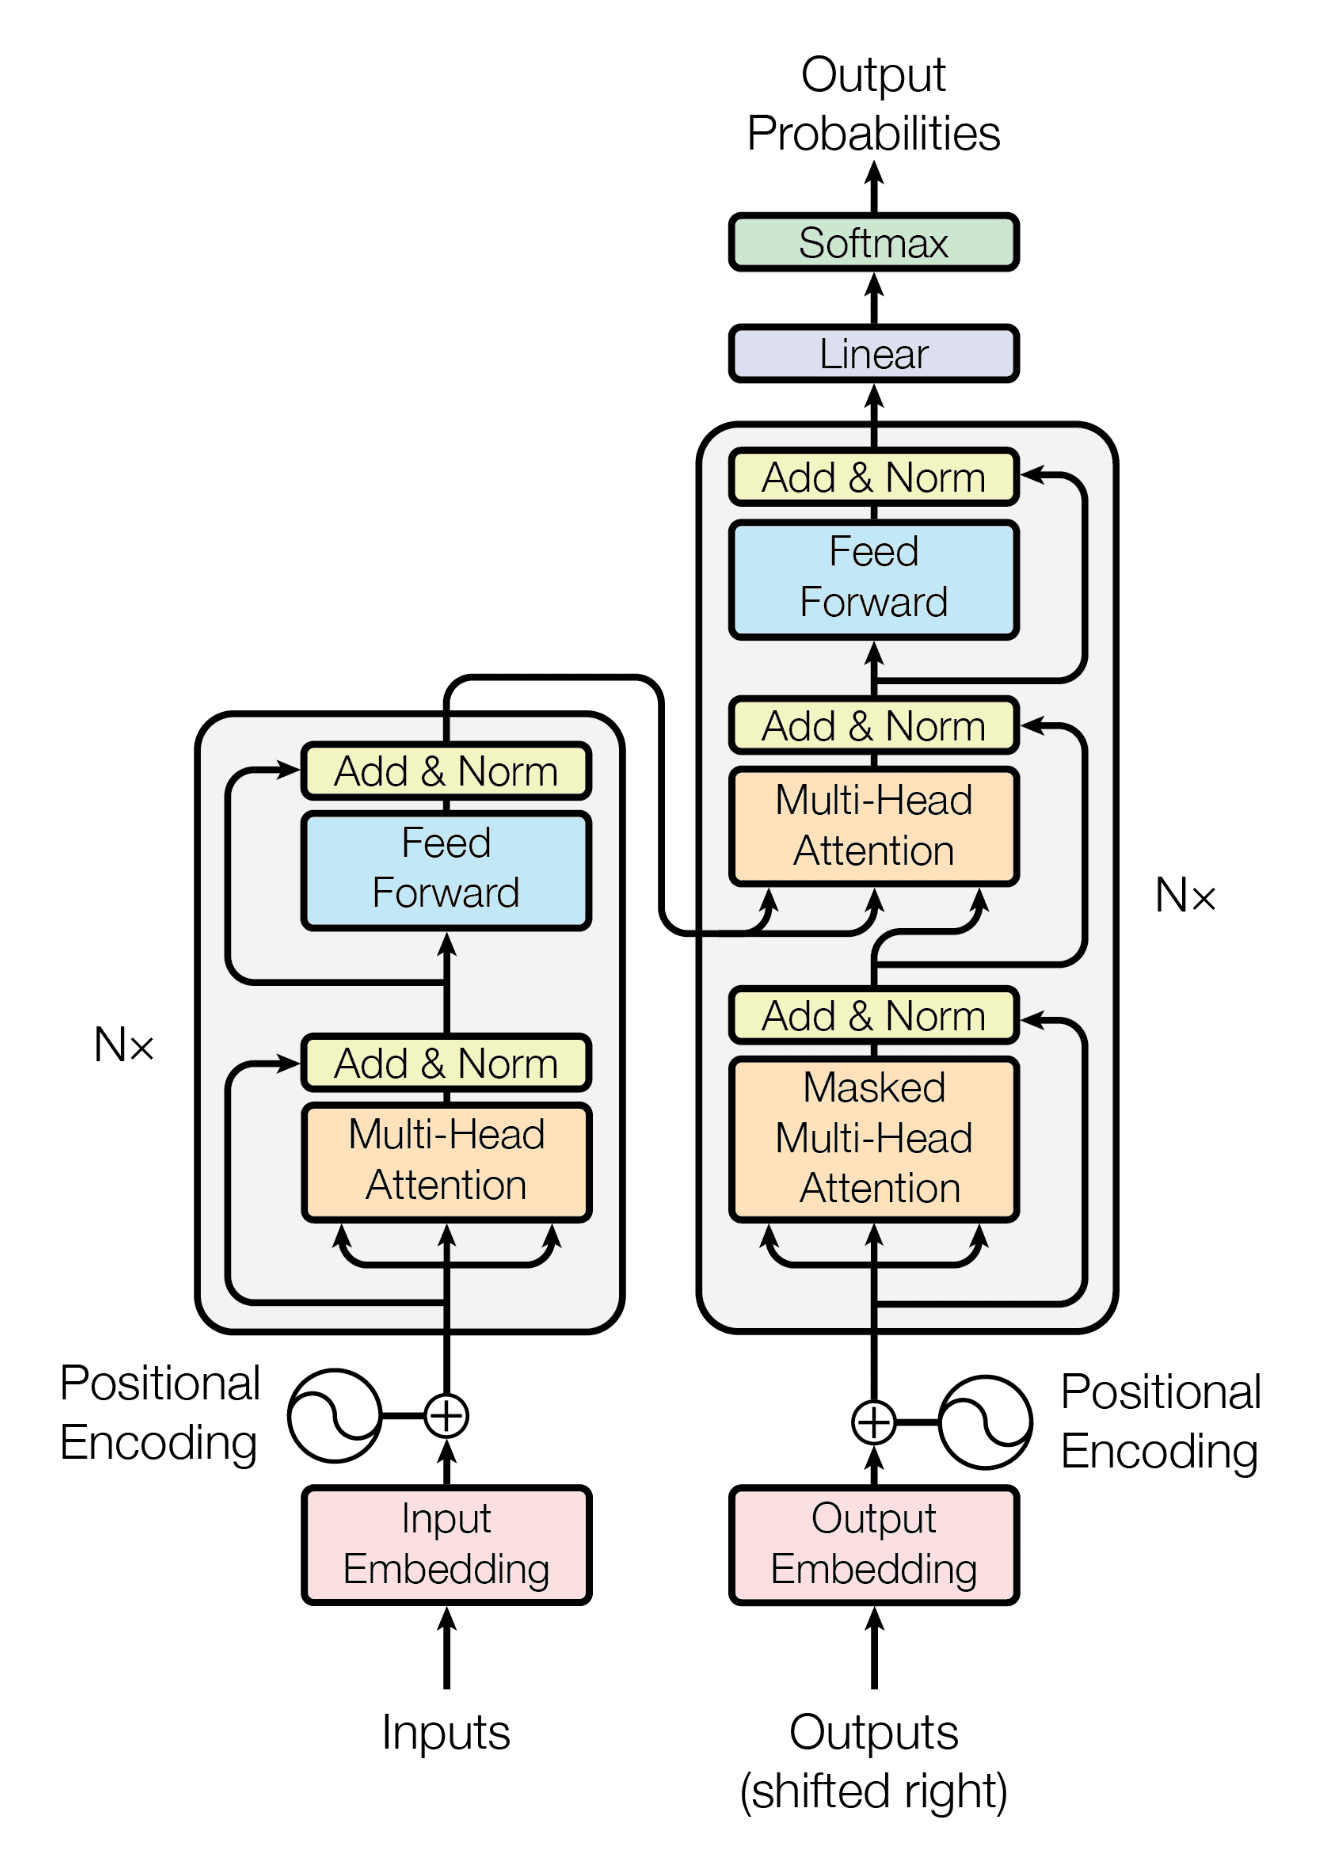
\includegraphics[scale=0.2]{img/attention_research_1}
	\caption{Transformer: modelo de arquitectura encoder-decoder \cite{vaswani2023attentionneed}}
	\label{trans}
\end{figure}  	

Su funcionamiento se basa en cuatro elementos, los cuales estudiaremos a continuación: su arquitectura basada en bloques encoder-decoder, la posiblidad de parelelizado mediante múltiples heads, el mecanismo de \textit{self-attention}, y la incorporación de información adicional mediante \textit{embeddings}, para así introducir información de orden, siendo este último el elemento que nos permitirá mejorar de manera drástica los resultados obtenidos al aplicar Transformers en series temporales.\\

A partir de ahora, nos centraremos en estudiar a fondo su aplicación y ajuste para tratar de mejorar los resultados obtenidos en series temporales.


\subsection{Conceptos previos: token y embedding}

En los modelos basados en Transformers, uno de los pasos principales antes de dotar la información a la arquitectura es transformar los datos en un formato numérico comprensible para la red neuronal. Esto es especialmente importante con textos, ya que tenemos la información codificada en caracteres.\\

Para construir las entradas, se emplea el concepto de \textit{token}, que representa la unidad mínima de entrada al modelo. Su tamaño depende del problema, y no existe una unidad cocnreta: podría ser una secuencia completa, una subpalabra, un carácter o incluso un símbolo de puntuación.\\

En su definición original para textos, el proceso de tokenización convierte una secuencia de texto en una lista de tokens, cada uno de los cuales es mapeado a un identificador entero a través de un vocabulario predefinido. Dicho mapeo sirve como base para generar una representación vectorial de cada token, conocida como \textbf{embedding}. Esta representación no se limita a un único vector, sino que resulta de la combinación de distintos componentes que aportan información contextual adicional.\\

En los modelos Transformer clásicos, cada token es transformado en un vector de entrada única de manera aditiva:

\begin{itemize}
	\item \textbf{Token embedding:} representa el significado semántico del token, aprendido durante el entrenamiento.
	\item \textbf{Positional encoding:} añade información sobre la posición del token en la secuencia, necesaria dado que los Transformers no procesan los datos de manera secuencial.
	\item \textbf{Segment embedding:} es un elemento opcional, el cual indica a qué segmento o frase pertenece cada token, útil en tareas de relación entre pares de oraciones.
\end{itemize}

La suma de estos tres vectores produce la entrada final que el modelo utiliza en la capa de atención, y permite que el modelo tenga acceso simultáneo tanto al contenido semántico como a la estructura secuencial del texto.\\

En el caso de las series temporales, el término token puede ser algo menos intuitivo de entender, ya que no tenemos palabras como tal. Pero cada punto temporal o ventana de datos puede considerarse una unidad equivalente. Aquí, el \textit{token embedding} suele derivarse directamente de los valores numéricos observados, y es la codificación posicional el elemento que cobra relevancia, ya que los valores de tiempo no están implícitos en la secuencia misma, sino que deben incorporarse explícitamente mediante un mecanismo que represente la fecha u hora.\\

De esta forma, podemos apreciar el paralelismo entre ambos dominios: mientras que en texto los embeddings representan palabras y estructuras lingüísticas, en series temporales encapsulan magnitudes numéricas y patrones temporales, pero dejando al margen la forma en la que construimos el embedding, en ambos casos buscamos representar y modelar las relaciones contextuales a lo largo del tiempo o de la secuencia.

\subsection{Arquitectura: encoder y decoder}

La arquitectura Transformer se construye sobre un esquema de tipo \textit{encoder–decoder}. Para comprenderlo mejor, podemos tomar como referencia los autoencoders, pero teniendo en cuenta que ahora nos centramos en el modelado de secuencias; mientras que un autoencoder clásico codifica una entrada en una representación latente para luego reconstruirla, el Transformer aplica esta idea para tareas de transformación de secuencia a secuencia: el encoder transforma la secuencia de entrada en una representación intermedia rica en contexto, y el decoder genera la secuencia de salida basada en dicha representación.

\subsubsection{Encoder}  
El encoder es la parte del modelo  que toma como entrada una secuencia de vectores (habitualmente embeddings de palabras o características de entrada), y produce una secuencia de vectores de igual longitud que contienen información contextualizada. Para aprovechar el paralelismo, está compuesto por una pila de $N$ bloques idénticos, donde cada uno incluye:

\begin{itemize}
	\item Un mecanismo de \textit{self-attention}, que permite a cada elemento de la secuencia atender a todos los demás y capturar relaciones globales, y cuyo funcionamiento profundizaremos posteriormente.
	\item Una red neuronal totalmente conectada, aplicada de manera independiente en cada posición.
\end{itemize}

Ambas subcapas están envueltas en una conexión residual seguida de una normalización por capas, de manera que no se produzca desvanecimiento de gradientes cuando tomamos largas secuencias de entrada, y además, se mejore la convergencia gracias al efecto de la normalización.

\subsubsection{Decoder}  
El decoder también consta de $N$ bloques, pero su estructura es ligeramente más compleja, ya que debe generar una secuencia salida de manera autoregresiva, que mantega la información contextual del orden. Cada bloque del decoder contiene:

\begin{itemize}
	\item Un \textit{self-attention} enmascarado. Su pricipal función es que el modelo, en un instante del proceso de predicción, pueda acceder a la información de tokens anteriores o a sí misma, pero no ver la información de tokens futuros.
	\item Un mecanismo de \textit{cross-attention}, que permite que cada token del decoder acceda a toda la información producida por el encoder, lo cual es esencial cuando existe una fuerte relación entre la información de entrada y la salida que se desea producir.
	\item Una red totalmente conectada de tipo feed-forward, similar a la del encoder.
\end{itemize}

Cada paso de generación en el decoder depende tanto de los tokens generados hasta el momento como de la representación completa de la entrada, por lo que se está aprovechando la información de orden existente en los datos y el conocimiento disponible, siendo este proceso totalmente compatible con la aplicación en series temporales.\\

Teniendo en cuenta el anterior símil del Transformer con los Autoencoders, es importante tener clara la diferencia para no entrar en cofusión. Aunque los Transformers no buscan reconstruir directamente la entrada como en los autoencoders clásicos, la estructura encoder–decoder cumple un propósito análogo: transformar información de entrada en una forma útil y compacta que el decoder pueda explotar para generar la salida deseada. A esta diferencia, se le suma también la utilidad de la información contextual: para mejorar el rendimiento, y facilitar el proceso de aprendizaje, el modelo hace uso de información que permita identificar relaciones de orden y facilitar el proceso de recurrencia de manera implícita en los datos.

\subsection{Mecanismo de atención}

El núcleo del Transformer es el mecanismo de \textit{self-attention}. Este se basa en la definición de 3 subespacios: Queries ($Q$), Keys ($K$) y Values ($V$). Profundizaremos en ver cómo se relacionan estos elementos desde un punto de vista formal.\\

La atención entre posiciones se calcula como una similitud entre queries y keys, seguida de una ponderación de los values:

\begin{equation}
	\text{Attention}(Q, K, V) = \text{softmax} \left( \frac{QK^T}{\sqrt{d_k}} \right)V
\end{equation}

Es frecuente encontrar en el denominador el término $\sqrt{d_k}$, ya que su principal función es evitar que los productos escalares sean excesivamente grandes, y actúa a modo de normalización para evitar problemas con los gradientes.\\

De por sí solo, este mecanismo es el principal elemento en el funcionamiento de los transformers. Pero podemos mejorar su potencial si lo paralelizamos. Es aquí cuando entra en acción el mecanismo de \textit{multi-head attention}, donde se realizan múltiples operaciones de atención en paralelo, cada una con sus propias proyecciones aprendidas, permitiendo al modelo aprender distintas relaciones entre tokens en diferentes subespacios de representación. 

\begin{equation}
	\text{MultiHead}(Q, K, V) = \text{Concat}(\text{head}_1, \ldots, \text{head}_h)W^O
\end{equation}

Posteriormente, estos valores se concatenan, y podemos obtener el resultado que buscábamos de manera paralela.


\subsection{Importancia del Positional Encoding}

Dado que el Transformer no incorpora mecanismos recurrentes ni convolucionales, carece de una forma intrínseca para captar el orden relativo o absoluto de los elementos que recibe como entrada. Para superar esta limitación, los autores del modelo original introdujeron el concepto de \textit{positional encodings}, vectores que se suman a las representaciones embebidas de cada token en función de su posición dentro de la secuencia. Estos vectores proporcionan una señal explícita de la ubicación de cada elemento, permitiendo que el modelo incorpore información posicional en el cálculo de la atención.\\

En el modelo original de transformer, el cual denominaremos en futuras secciones como Transformer \textit{vanilla}, el positional encoding se definió mediante funciones periódicas basadas en seno y coseno con distintas frecuencias, cuya formulación es la siguiente:

\begin{equation}
	\text{PE}_{(pos, 2i)} = \sin\left( \frac{pos}{10000^{2i/d_{\text{model}}}} \right)
\end{equation}
\begin{equation}
	\text{PE}_{(pos, 2i+1)} = \cos\left( \frac{pos}{10000^{2i/d_{\text{model}}}} \right)
\end{equation}

Este diseño ofrece varias ventajas: al ser funciones periódicas y deterministas, no requieren parámetros adicionales a entrenar y permiten que el modelo generalice a secuencias más largas que las vistas durante el entrenamiento. Además, facilitan que la red aprenda a reconocer patrones posicionales y relaciones relativas entre elementos, aprovechando las propiedades de las ondas seno y coseno para captar distancias y ciclos.\\

No obstante, aunque esta técnica es adecuada para procesar texto, donde el orden es fundamental, su aplicabilidad en series temporales es más compleja y no siempre ha de producir un buen resultados. En las series temporales, la posición en la secuencia no es solo un índice ordinal, sino que representa una dimensión temporal real, ligada a un instante específico. Esto implica que los elementos de la secuencia deben ordenarse dado su timestamp, pero también contienen información contextual inherente al tiempo: estacionalidad, tendencias que evolucionan a lo largo del tiempo, y eventos que ocurren en momentos concretos.\\

En las series temporales, cuando queremos detectar sucesos concretos o anomalías, para posteriormente modelar y crear predicciones largo plazo, toda la información no suele estar concentrada en único timestamp. Por ejemplo, si tenemos un dataset muestreado por horas, puede ser frecuente y viable que para comprender el fenómeno, debamos mirar no sólo la información de una hora concreta, sino del día completo. Por tanto, la codificación posicional tradicional basada en seno y coseno no captura explícitamente estas características, pues si bien es capaz de establecer un orden en el punto de vista global de los datos, no es capaz de contener y explicar información local de estos. 	Estamos perdiendo información contenida en patrones temporales más complejos.\\

Esto plantea un desafío fundamental: la necesidad de diseñar o adaptar mecanismos de \textit{positional encoding} que sean capaces de integrar no solo la información ordinal, sino también las propiedades temporales explícitas que caracterizan a estos datos. En el estado del arte, podemos encontrar ya algunos enfoques en esta dirección:

\begin{itemize}
	\item \textbf{Encodings aprendibles}. Permiten al modelo optimizar vectores posicionales específicos para las características del conjunto de datos. Tienen la ventaja de facilitar el proceso de entrenamiento sin necesidad de especificar parámetros de forma explícita, pero se debe tener especial cuidado con la inicialización y la normalización de valores, para evitar problemas de crecimiento desproporcionado en ciertos parámetros.
	\item \textbf{Codificaciones basadas en atributos del timestamp}. Consiste en incluir explícitamente variables de tiempo (hora, día de la semana, mes, año) que añaden señales temporales al embedding, de forma que se pueda usar su información para el orden, pero también como un atributo más del problema.
	\item \textbf{Transformaciones basadas en series de Fourier o wavelets}. Capturan patrones periódicos más complejos y multi-escalares, aunque, dada su naturaleza basada también en funciones trigonométricas, acercan la codificación a los datos pero sigue siendo un enfoque similar al original con sus correspondientes limitaciones.
\end{itemize}

Aunque se han logrado mejoras y avances sobre la definición vanilla del encoding posicional gracias a estas propuestas, la mayoría de estas aproximaciones comparten una limitación estructural: la escasa vinculación semántica y local entre los datos de entrada y su codificación posicional.\\

De manera más detallada, frecuentemente los vectores que representan la posición suelen ser generados de forma independiente al contenido real de la secuencia. Esto significa que dos tokens o timestamp con significado similar pero ubicados en posiciones diferentes reciben representaciones posicionales completamente distintas, sin ningún tipo de correspondencia semántica entre ellas. En series temporales, puede suponer un grave problema: encontrar patrones como la estacionalidad pueden ser claves en el modelado, y con este enfoque, este tipo de ciclos sería prácticamente imposible de detectar.\\

Un ejemplo sencillo podría ser la estimación del consumo eléctrico. En una serie que recoge datos meteorológicos diarios durante varios años, los valores correspondientes a una hora concreta de diferentes días podrían compartir patrones similares; es habitual encontrar por ejemplo consumos superiores en las horas cercanas al almuerzo o la cena, y de menor uso en altas horas de la madrugada. Pero, si la codificación posicional no reconoce esta regularidad por tratarse de posiciones globalmente distintas en la secuencia, el modelo no podrá aprovechar dicha repetición estructural, limitando su capacidad de modelado.\\

Además, en muchos contextos, los eventos relevantes están más determinados por la posición relativa y el entorno local inmediato que por una posición absoluta dentro de la secuencia. La falta de mecanismos que conecten directamente el significado de los datos con su ubicación limita el poder expresivo de la red y su capacidad para realizar generalizaciones útiles. Esta problemática refuerza la necesidad de proponer codificaciones posicionales con mayor semántica, más contextualizadas, que integren explícitamente el contenido de los datos y su estructura temporal.\\

En el apartado siguiente, estudiaremos los modelos más relevantes del estado del arte, y analizaremos en qué característica clave se basa cada uno de ellos. Además, prestaremos atención a qué tipo de codificación emplea cada uno, de cara a obtener conclusiones sobre la importancia general que se le da a este aspecto.

\subsection{Modelos aplicados al forecasting de series temporales}

En el estado del arte, podemos encontrar multitud de modelos que proponen adaptaciones y soluciones alternativas al uso de Transformers para series temporales. Algunas, son soluciones propias de lenguaje natural adaptadas a su uso en series temporales, mientras que en otros casos tratan de basarse en conceptos básicos anteriormente explotados en series, como la descomposición o el uso de la autocorrelación, pero empleando Transformers como vía de aprendizaje.\\

Concretamente, comenzaremos analizando variantes del modelo Transformer original que tuvieron un gran impacto en los modelos adaptados, como TransformerXL \cite{dai2019transformerxlattentivelanguagemodels}, Reformer \cite{kitaev2020reformerefficienttransformer} y LogTrans~\cite{NEURIPS2019_6775a063}, para posteriormente analizar el funcionamiento de Informer~\cite{zhou2021informerefficienttransformerlong}, Autoformer~\cite{wu2022autoformerdecompositiontransformersautocorrelation}, FEDFormer~\cite{zhou2022fedformerfrequencyenhanceddecomposed}, y modelos más recientes como PatchTST~\cite{nie2023timeseriesworth64} y TimesNet~\cite{wu2023timesnettemporal2dvariationmodeling}.

\subsubsection{Variantes de Transformer y mejoras previas}

El modelo original de Transformer propuesto en \textit{Attention is All You Need} \cite{vaswani2023attentionneed} ha sido objetivo de muchas investigaciones que han buscado optimizar tanto la capacidad de modelado como la eficiencia computacional. Si bien su principal campo de aplicación siguió siendo el lenguaje natural, dichas innovaciones han permitido posteriores mejoras a las aplicaciones de Transformers en series temporales.\\

De entre las características deseables, se han buscado continuamente mejoras de rendimiento para dominios de larga secuencia, relaciones de dependencia a múltiples escalas y mejoras a nivel computacional, tratando de reducir la complejidad de ejecución pero sacrificando el mínimo rendimiento posible.

\paragraph{Transformer-XL (2019)}


Una de las primeras propuestas realizadas es el Transformer-XL \cite{dai2019transformerxlattentivelanguagemodels}. Esta profundiza sobre el concepto de positional encoding relativo, reemplazando el esquema absoluto original por uno que codifica distancias relativas entre tokens. Esto no solo permite capturar mejor dependencias a largo plazo, sino que también hace posible extender el contexto más allá de la ventana de entrenamiento, reutilizando estados ocultos de segmentos previos y patrones locales.\\

En series temporales, esta técnica tiene una gran relevancia en la detección de patrones estacionales, ya que nos permite encontrar patrones, donde el significado de la relación temporal radica sobre todo en dónde se ubica un evento concreto dentro del período estacional, y no tanto en su posición absoluta en la secuencia.

\newpage
\paragraph{LogTrans (2019)}

La variante LogTrans\cite{NEURIPS2019_6775a063} se centra en reducir el coste computacional del cálculo de atenciones, proponiendo un mecanismo de atención diseñado para reducir el coste computacional del \textit{self-attention} tradicional, denominado \textit{log-sparse attention}. La idea busca su fundamento en secuencias de larga extensión, donde se argumenta que no todas las interacciones entre elementos son igualmente relevantes: mientras que ciertas posiciones requieren una atención densa hacia elementos cercanos, por razones como lazos locales estrechos, otras mantienen dependencias más espaciadas que solo necesitan ser consideradas de forma ocasional. Para lograrlo, el mecanismo \textit{log-sparse} selecciona las posiciones a las que cada token presta atención siguiendo una distribución logarítmica. Esto significa que las posiciones cercanas se incluyen de forma continua y densa, asegurando que las dependencias locales estén bien representadas, mientras que las posiciones más lejanas se muestrean con menor densidad, manteniendo aún así una cobertura global de la secuencia pero con un número significativamente reducido de interacciones.\\

Empleando el muestreo, la complejidad se reduce de \(O(n^2)\) a aproximadamente \(O(n \log n)\), lo que permite manejar secuencias mucho más largas sin que el coste computacional o el consumo de memoria GPU se disparen. Sin embargo, esta estrategia tiene ciertos riesgos, sobre todo si lo aplicamos a series temporales: usar un patrón de muestreo conlleva el riesgo de perder información relevante, ya que dicha relación no está siendo recogida. Este problema puede resultar especialmente crítico en series temporales donde ciertas fluctuaciones clave puedan ser omitidas y provoquen una pérdida de rendimiento considerable, o bien, durante la búsqueda de anomalías en las series, tarea la cual está bastante vinculada también con la predicción.\\

A pesar de esta limitación, \textit{log-sparse attention} demostró que es posible reducir el coste de la atención a cambio de un pequeño incremento del error en series, siendo más notable en series de larga extensión. De hecho, esta idea abrió la puerta a modelos como \textit{Informer}, uno de los modelos de \textit{forecasting} basados en Transformers más influyentes en el estado del arte,  en el que se adopta el enfoque probabilístico para seleccionar las claves más relevantes. Más adelante, examinaremos su funcionamiento en detalle, centrándonos en su aplicación específica a la predicción de series temporales.

\paragraph{Reformer (2020)}

Reformer \cite{kitaev2020reformerefficienttransformer} aborda otro de los cuellos de botella principales de los Transformer: el coste $O(n^2)$ del cálculo de atenciones. En secuencias muy largas, el orden cuadrático puede aumentar considerablemente los tiempos de ejecución, hasta el punto de que en datasets de gran tamaño, puede suponer un obstáculo de cara a poder ser ejecutado. Dicho orden de complejidad proviene de realizar el producto entre los diferentes tokens de entrada, pues se debe realizar el producto de cada elemento por el resto, y esto depende directamente del tamaño de los datos.\\


Para tratar de reducir dicha complejidad, Reformer introduce varios conceptos fundamentales que mejoran la eficiencia sin sacrificar la calidad del aprendizaje.

\begin{itemize}
	\item \textbf{Locality-Sensitive Hashing (LSH):} Esta técnica permite aproximar el cálculo de la atención agrupando tokens similares mediante el uso de funciones hash, diseñadas para preservar la proximidad en el espacio vectorial. En lugar de calcular la atención entre todos los pares de tokens, el modelo solo la calcula dentro de unos grupos, llamados \textit{buckets}, que están formados por tokens cercanos en su representación (ver figura \ref{reformer}).
	
	Gracias a ello, podemos reducir el coste de \(O(n^2)\) a aproximadamente \(O(n \log n)\), al limitar las interacciones a subconjuntos relevantes. Además, LSH favorece que la atención se concentre en relaciones locales y semánticamente relevantes, lo cual favorece también colateralmente a su aplicación en series temporales y la detección de estacionalidad.
	
	\begin{figure}[!ht] %con el [H] le obligamos a situar aquí la figura
		\centering
		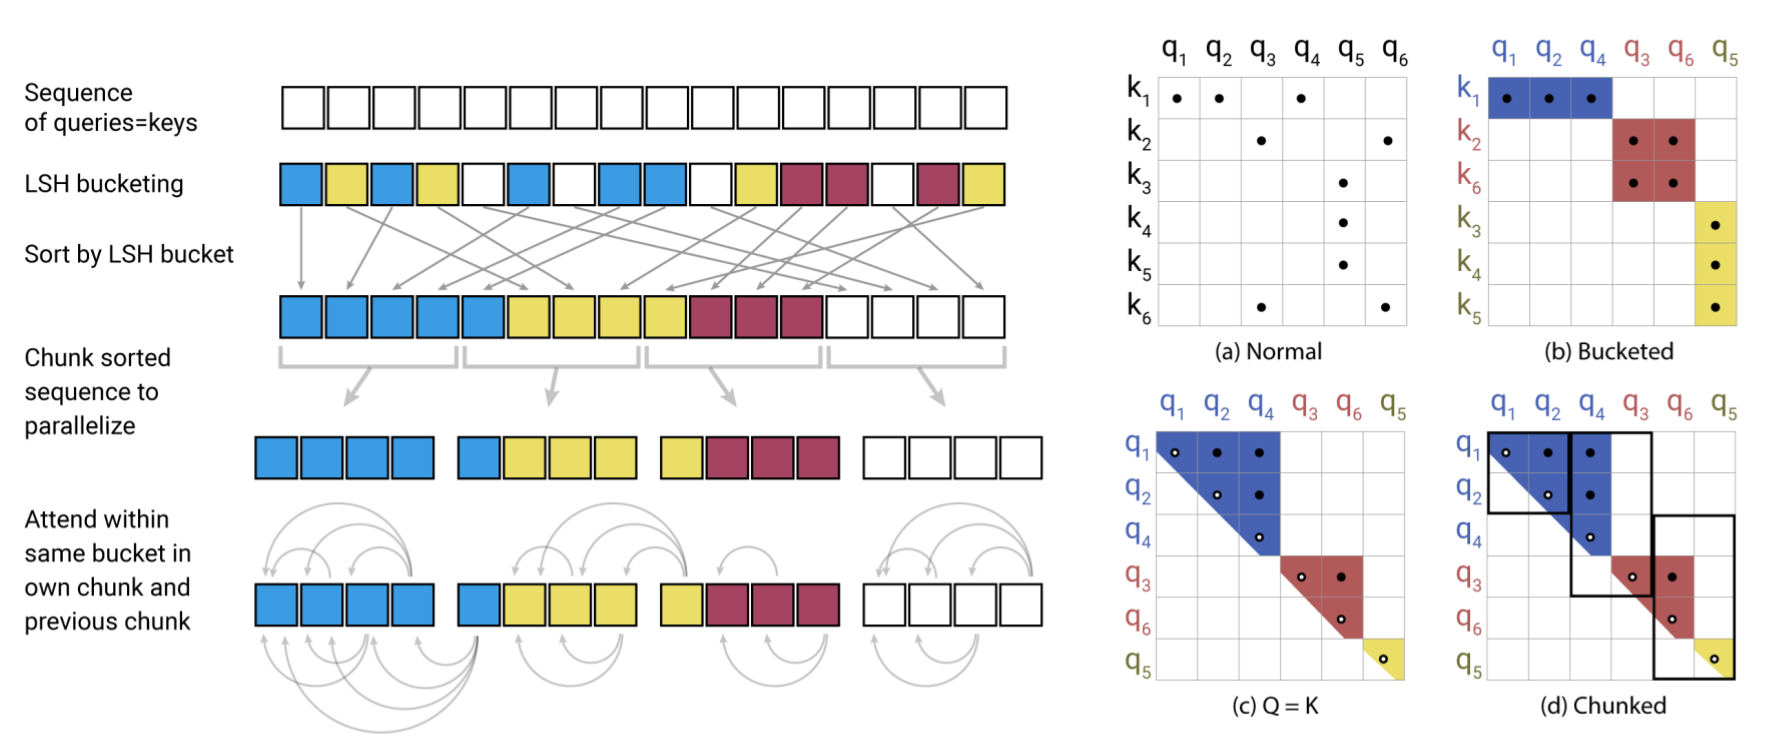
\includegraphics[scale=0.225]{img/reformer}
		\caption{Reformer: funcionamiento del mecanismo de creación de \textit{buckets} \cite{kitaev2020reformerefficienttransformer}}
		\label{reformer}
	\end{figure}  	
	
	\item \textbf{Codificación reversible:} Continuando con las mejoras de eficiencia, Reformer modifica la arquitectura para emplear redes residuales reversibles que permiten reconstruir los estados intermedios de cada capa durante \textit{backpropagation}, en lugar de almacenarlos durante el \textit{forward}. Esto reduce drásticamente la memoria requerida para entrenar modelos profundos y secuencias largas. La invertibilidad de las capas permite recuperar el input de cada capa a partir de su output, lo que implica una compensación entre tiempo computacional (por el costo de recalcular estados) y memoria. Su impacto puede apreciar en mayor medida cuando el conjunto de entrada dispone miles o millones de instancias o pasos a analizar.
	
\end{itemize}

Ambas mejoras nos permiten realizar un mejor aprovechamiento de la memoria de video, mejorando la reutilización de cálculos y permitiendo así usar conjuntos de datos de mayor tamaño, aunque debemos de tener en cuenta que agrupar por similaridad introduce errores numéricos en el cálculo de la atención.

\subsubsection{Informer (2020)}

El modelo Informer~\cite{zhou2021informerefficienttransformerlong} es una de las primeras propuestas que adapta de forma específica la arquitectura Transformer al dominio de las series temporales, tratando de modificar su funcionamiento para adaptarse a las limitaciones detectadas en el contexto de series temporales. Su diseño se orienta al problema de \textit{Long Sequence Time-Series Forecasting} (LSTF), para predecir horizontes temporales largos a partir de entradas igualmente extensas, lo que plantea dificultades de escalabilidad y eficiencia tanto en entrenamiento como en inferencia.\\

En el uso directo de Transformers canónicos sobre series temporales, surgen tres problemas fundamentales, algunos de ellos ya estudiados en el apartado anterior:

\begin{itemize}
	\item \textbf{Alta complejidad computacional y de memoria}. La implementación estándar del mecanismo de atención presenta un coste de $O(L^2)$ en secuencias de longitud $L$, debido a la necesidad de calcular interacciones entre todos los pares de posiciones. Esto limita su uso en horizontes de predicción largos o datos de alta frecuencia, ya que limita su escalabilidad.
	\item \textbf{Cuellos de botella con la memoria}. En arquitecturas encoder–decoder profundas, donde tenemos varias capas, podemos tener problemas con la complejidad espacial, ya que disponiendo de $J$ capas, la complejidad total será de $O(J \cdot L^2)$, limitando así la posibilidad de procesar largas series.
	\item \textbf{Baja velocidad de inferencia}. En la inferencia original propuesta por Transformer, el decoding se realiza paso a paso, aumentando los tiempos de inferencia hasta el punto de ser tan lenta como los modelos basados en RNN. Por tanto, debemos de encontrar un nuevo mecanismo capaz de simplificar y adaptar este proceso.
\end{itemize}

Para mitigar estas limitaciones, Informer introduce tres innovaciones clave:

\begin{enumerate}
	\item \textbf{ProbSparse Self-Attention}. Se trata de un mecanismo de atención dispersa basado en la hipótesis de que, en muchas tareas de series temporales, solo unas pocas \textit{queries} concentran la mayor parte de la relevancia en la atención. Al muestrear y priorizar dichas \textit{queries}, se reduce el coste computacional de $O(L^2)$ a $O(L\log L)$ sin degradar la capacidad de modelar dependencias a largo plazo. Para ello, se emplea el mismo procesamiento visto en LogTrans \cite{NEURIPS2019_6775a063}.
	\item \textbf{Self-Attention Distilling}. Se trata de una operación jerárquica que filtra las atenciones dominantes y reduce progresivamente la dimensión temporal entre capas. Este proceso actúa como una mecanismo de compresión, donde se preservan los patrones relevantes y disminuyendo el consumo de memoria, permitiendo que modelos más profundos procesen secuencias largas sin sobrecargar la GPU, logrando una complejidad reducida de $O( (2 - \epsilon) L \log L)$.
	\item \textbf{Generative Decoder}. Para solucionar el problema de la inferencia paso a paso, se propone un decodificador capaz de generar toda la secuencia de salida en un único paso (\textit{one-forward}). Este enfoque no solo acelera la inferencia, sino que también reduce la acumulación de errores entre pasos, mejorando la estabilidad en horizontes de predicción extensos.
\end{enumerate}

En conjunto, estas mejoras convierten a \textbf{Informer} en un modelo especialmente interesante para escenarios de predicción multivariados y datos de gran volumen, manteniendo la capacidad de capturar tanto dependencias locales como globales reduciendo el impacto en memoria y mejorando la eficiencia.\\

A continuación, haremos énfasis en cada una de estas 3 propuestas, y analizaremos por partes su arquitectura (ver figura \ref{informer}).

\begin{figure}
	\centering
	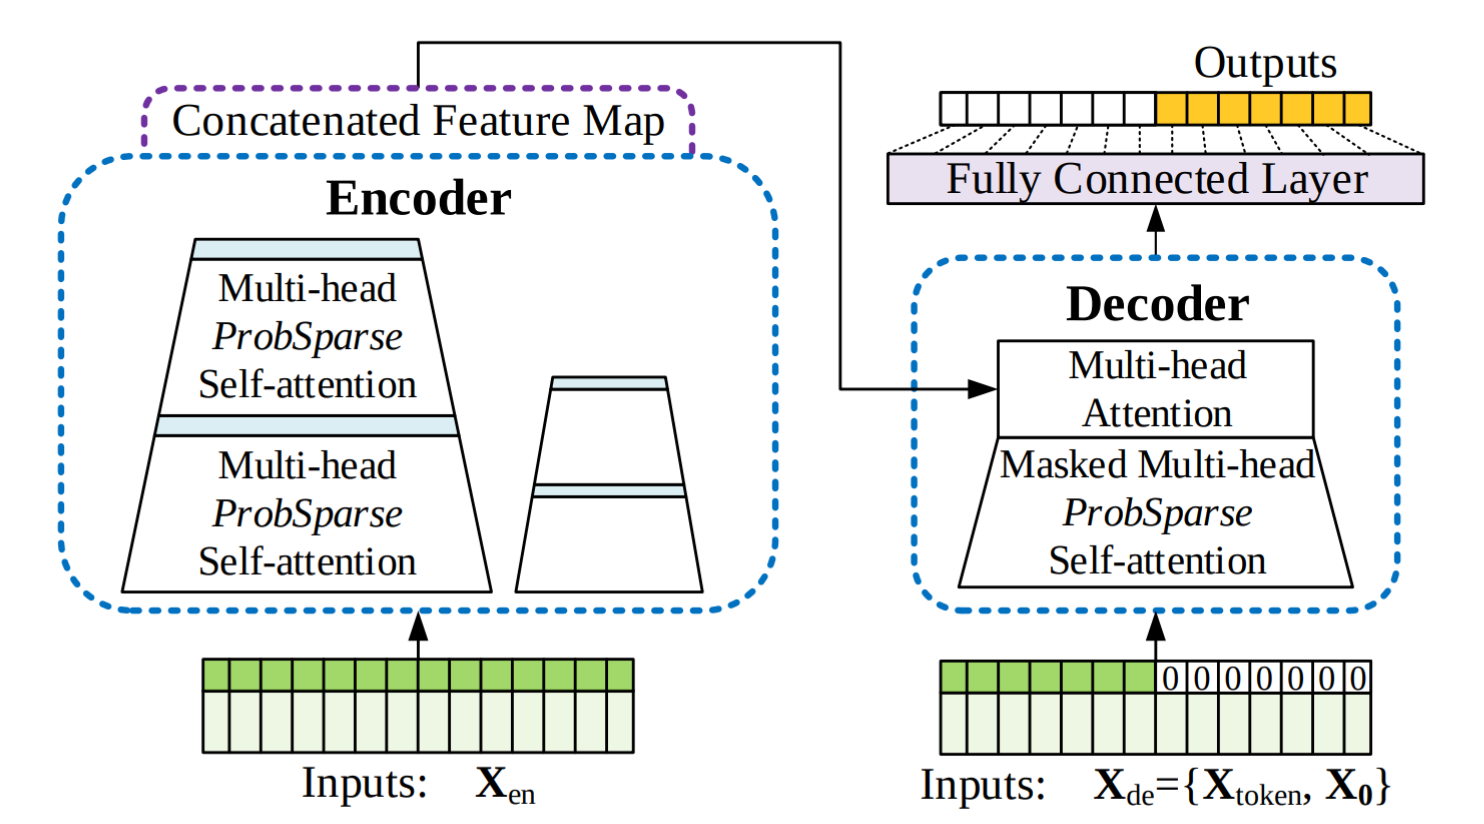
\includegraphics[scale=0.25]{img/informer.png}
	\caption{Informer: arquitectura completa del modelo~\cite{zhou2021informerefficienttransformerlong}}
	\label{informer}
\end{figure}

\paragraph{Mecanismo de atención}

El mecanismo de \textit{self-attention} tradicional se definía como:
\begin{equation}
	A(Q,K,V) = \operatorname{Softmax}\!\left( \frac{QK^\top}{\sqrt{d}} \right) V,
\end{equation}

Donde la implementación canónica requiere computar todas las similitudes par a par \(QK^\top\), con coste temporal y de memoria \(O(L^2)\).

Informer parte de la observación empírica de que la distribución de probabilidades de atención suele mostrar una \textit{cola larga}: pocas consultas concentran la mayor parte de la energía de atención, mientras que la mayoría producen señales débiles. Para aprovechar esta propiedad, se define una medida de ``dispersión de consulta'' que cuantifica la propensión de una consulta \(q_i\) a generar picos de atención:

\begin{equation}
	M(q_i,K) \;=\; \max_j \left\{ \frac{q_i k_j^\top}{\sqrt{d}} \right\} \;-\; \frac{1}{L_K} \sum_{j=1}^{L_K} \frac{q_i k_j^\top}{\sqrt{d}},
\end{equation}

donde \(L_K\) es el número de claves (en encoder–decoder \(L_Q\) y \(L_K\) pueden diferir). Intuitivamente, \(M(q_i,K)\) mide la diferencia entre el máximo score y el score medio: valores grandes indican consultas con picos pronunciados (es decir, consultas ``informativas'').

Esencialmente, este mecanismo consta de dos fases:
\begin{enumerate}
	\item \textbf{Selección de consultas relevantes:} se estima \(M(q_i,K)\) mediante muestreo parcial de claves con LogSparse y se conservan solo las \(u = c \cdot \ln L_Q\) consultas con mayor valor.
	Para ello, para cada consulta \(q_i\), se calcula una estimación de su medida de dispersión
	\begin{equation}
		\hat{M}(q_i, K) = \max_{j \in \mathcal{S}_i} \left\{ \frac{q_i k_j^\top}{\sqrt{d}} \right\} - \frac{1}{|\mathcal{S}_i|} \sum_{j \in \mathcal{S}_i} \frac{q_i k_j^\top}{\sqrt{d}},
	\end{equation}
	donde \(\mathcal{S}_i \subset \{1, \dots, L_K\}\) es un subconjunto de claves obtenido mediante muestreo \textit{log-sparse}, es decir, seleccionando índices de forma que la densidad de puntos crece logarítmicamente con la distancia temporal.  
	Este muestreo permite aproximar \(M(q_i, K)\), tratando de mantener con alta probabilidad las claves más informativas. 
	
	Finalmente, se ordenan las consultas según \(\hat{M}(q_i, K)\) y se conservan solo las \(u = c \cdot \ln L_Q\) de mayor valor, donde \(c\) establece qué proporción seleccionar. A mayor valor, mayor precisión, pero mayor coste.
	
	\item \textbf{Cálculo selectivo de atención:} solo para esas \(u\) consultas se computa la atención completa frente a todas las claves, mientras que las no seleccionadas reciben una aproximación suave o interpolada. Esta podría ser un valor medio, ya calculado anteriormente al realizar la búsqueda de las instancias informativas.
\end{enumerate}

Con \(u = O(\log L)\), el coste se reduce de \(O(L^2)\) a \(O(L \log L)\) por cada head del modelo, consiguiendo una reducción considerable de la complejidad.

\paragraph{Distilling}

En el \textit{encoder} de Informer, la secuencia de entrada \(X^{en} \in \mathbb{R}^{L_x \times d_{model}}\) atraviesa múltiples capas de \textit{ProbSparse self-attention}, extrayendo dependencias relevantes entre los elementos temporales.\\

Sin embargo, procesar de forma directa secuencias largas en todas las capas genera un elevado coste computacional y de memoria.  
Para mitigar este problema, los autores introducen un bloque intermedio de \textit{distilling}, cuyo objetivo es reducir progresivamente la longitud temporal mientras se conservan las representaciones más relevantes.\\

Tras cada capa de atención, se aplica el bloque de \textit{distilling}, compuesto por una convolución 1D, una activación no lineal ELU y un \textit{max pooling} con paso 2:

\begin{equation}
	X^{t}_{j+1} = \text{MaxPool} \left( \text{ELU} \left( \text{Conv1d}([X^t_j]_{AB}) \right) \right),
\end{equation}

donde \([X^t_j]_{AB}\) denota la salida del bloque de atención multi-cabeza \textit{ProbSparse} combinada con conexiones residuales y normalización por capas (ver figura \ref{distilling})

\begin{figure}[!ht]
	\centering
	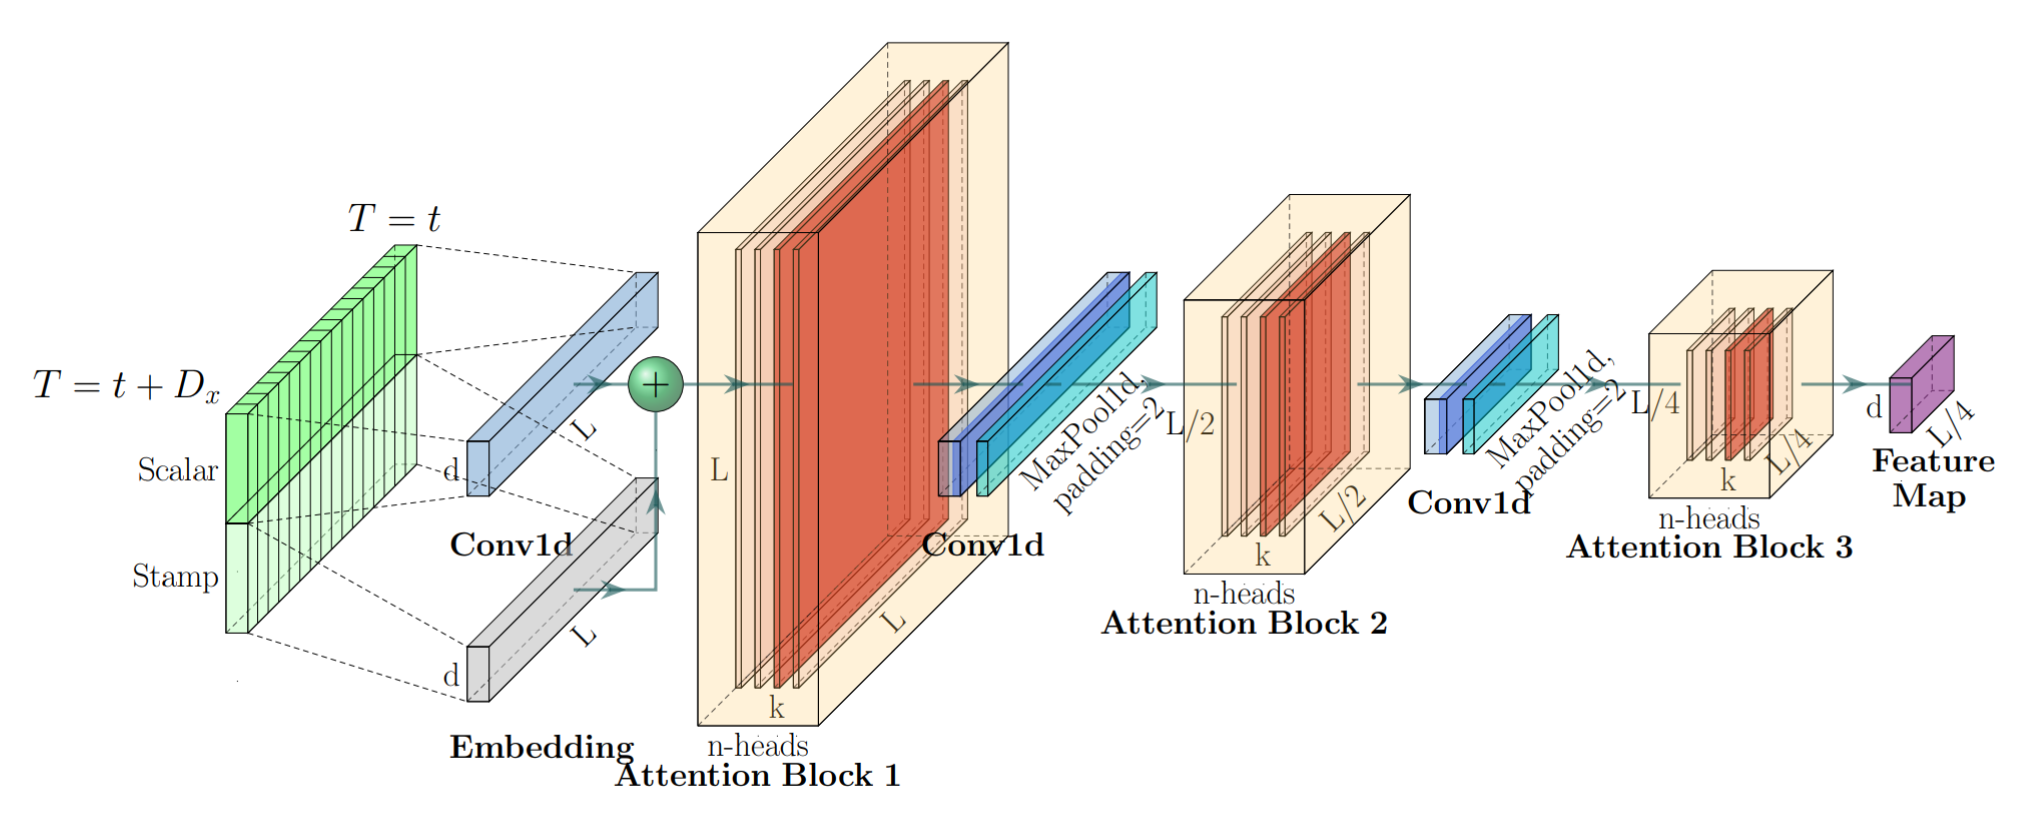
\includegraphics[scale=0.2]{img/distilling.png}
	\caption{Informer: procesamiento seguido durante el distilling~\cite{zhou2021informerefficienttransformerlong}}
	\label{distilling}
\end{figure}
Este proceso cumple dos funciones clave; por un lado, trata de filtrar las relaciones importantes. Al reducir la longitud temporal, se atenúan las interacciones menos relevantes, conservando únicamente las representaciones que concentran la mayor parte de la atención. Como se aplica un MaxPooling de 2,  la reducción de la secuencia a la mitad en cada paso disminuye el coste espacial hasta \(O((2 - \varepsilon) L \log L)\), reduciendo notablemente la complejjidad del encoder. \\

Para mejorar aún más la capacidad de capturar relaciones en distintas escalas temporales, se utilizan réplicas de \textit{stacks} del encoder con diferentes longitudes de entrada (por ejemplo, en la figura \ref{distilling}, \(L\), \(L/2\) y \(L/4\)), cuyos resultados se concatenan antes de las etapas finales. Este enfoque multi-escala es especialmente útil para detectar patrones que se repiten en diferentes horizontes.

\paragraph{Decodificación. Inferencia en un solo paso}

El decoder de Informer, sin entrar en particularidades concretas de cada capa, cumple con la arquitectura de un \textit{Transformer decoder} vanilla, pues posee en su definición dos capas de atención multi-cabeza: la primera opera de forma enmascarada sobre la secuencia objetivo parcial y la segunda aplica atención cruzada sobre las salidas del encoder.\\

Sin embargo, introduce una modificación crucial en el proceso de inferencia que lo diferencia de los enfoques autoregresivos tradicionales: en lugar de generar la salida paso a paso, acumulando potencialmente errores en cada predicción intermedia, el decoder de Informer adopta un esquema de inferencia en un solo paso, al estilo de los modelos generativos.\\

Para ello, se insertan una serie de elementos que simplifican el proceso. Este comienza concatenando construyendo el formato de entrada del modelo, que consta de una sección de datos de entrada, una ventana de contexto conocida, el cual llamaremos token de contexto, de longitud $L_{\text{token}}$, con un bloque de posiciones objetivo inicialmente vacías $X_0$:

\[
X^{de} = \text{Concat}(X^{\text{token}}, X_0) \in \mathbb{R}^{(L_{\text{token}} + L_y) \times d_{\text{model}}},
\]

donde $L_y$ es la longitud de la secuencia que se desea predecir.  Lo que se persigue es que tras el token de contexto, dichos ceros se vean sustituidos por la predicción realizada por  el modelo.

A través de los mecanismos de enmascaramiento, ya presentes en el Transformer original, el modelo solo podrá acceder a información presente en posiciones anteriores o del \textit{contexto inicial}, evitando el acceso a valores futuros.\\

Tras el paso por las capas de atención y normalización, una capa totalmente conectada proyecta directamente toda la secuencia objetivo de salida en un único cálculo, eliminando así la necesidad de decodificación iterativa. De esta forma, conseguimos, por un lado, reducir el tiempo de inferencia, y por otro, mitigar la acumulación de errores típica de modelos autoregresivos, mejorando la estabilidad y la precisión en predicciones de horizontes largos.

\paragraph{Análisis crítico y conclusiones}
Tras analizar el funcionamiento de este modelo, podemos apreciar que los avances realizados en su publicación fueron clave para realizar una adaptación de los Transformers a series temporales. Gracias al mecanismo de distillation, podemos simplificar progresivamente la arquitectura y encontrar patrones en diferentes grados de escala, y el mecanismo de predicción e inferencia tiene mucho más sentido que el mecanismo autoregresivo original, ya que así conseguimos resolver el problema del error acumulado que ya encontramos cuando aplicamos modelos clásicos como ARIMA.\\

Sin embargo, siendo críticos, podemos encontrar algunas decisiones controvertidas. En primer lugar, Informer no altera el proceso de codificación posicional de los Transformer de manera significativa, ya que por defecto, opera con la tradicional codificación sinusoidal, la cual es bastante rígida. Sólo depende de la longitud de la secuencia, pero no se adapta a su comportamiento o entorno, por lo que no estamos añadiendo información útil a nivel local de la serie, dificultando la detección de patrones estacionales o elementos de interés como  anomalías.\\

Por otro lado, la selección de instancias mediante LogSparse para simplificar la complejidad del cálculo de atención puede ser problemática. Aunque la teoría propuesta tiene sentido, ya que se afirma que no todos los puntos tienen la misma importancia, y que la selección probabilística da como resultado un vector ordenado de elementos por importancia \textit{M}, realmente es una asunción demasiado fuerte. Es posible que, en series temporales medidas en cortos períodos, como segundos o minutos, y duración extensa del fenómeno, como meses o años, los cambios apreciados en gran cantidad de puntos no sean especialmente relevantes, pues quizás la granularidad es demasiado pequeña. Pero en datasets que estudien fenómenos cortos y cambiantes, que ocurren a gran velocidad, como detección de fallos en tiempo real, o estudio de fenómenos como sistema de seguridad de centrales nucleares, (es decir, entornos industriales), puede que estemos eliminando puntos de interés.\\

La selección aleatoria mediante una distribución logarítmica, si bien es útil e interesante desde el punto de vista de la complejidad computacional, a nivel semántico puede alejarse bastante del problema que se está estudiando. El muestreo aleatorio puede distanciar al modelo de la estructura real del problema, ignorando relaciones locales o patrones que podrían ser relevantes para nuestra tarea.\\

Algo similar ocurre con los mecanismos de reducción temporal basados en \textit{Max Pooling}, en la etapa de \textit{distilling}. Reducir a la mitad la longitud de la secuencia en cada capa implica que, a la pérdida de información ya sufrida en el muestreo, se añade el riesgo de eliminar instancias que habían sido consideradas relevantes en pasos anteriores, y dar lugar a que ciertas posiciones del modelo mantengan valores por defecto o información incompleta y se desperdicie aún más información útil.

\subsubsection{Autoformer (2021)}

Tras la formulación del Transformer original, siguen surgiendo modelos y adaptaciones de Transformer para aplicar con series temporales. Uno de los siguientes es Autoformer~\cite{wu2022autoformerdecompositiontransformersautocorrelation}, el cual realiza un cambio de vista total con respecto a Informer. A diferencia de este último, que trataba de eliminar la autocorrelación por el riesgo de errores acumulativos en el decoder, Autoformer basa su funcionamiento esencial precisamente en la autocorrelación, y recuperando uno de los elementos característicos de los primeros algoritmos de procesamiento de series temporales: la descomposición.\\

Continuando con la tarea de predicción LSTF, Autoformer trata de solucionar dos problemas particulares de esta tarea. En primer lugar, la dificultad para identificar dependencias fiables en horizontes extensos, donde los patrones temporales suelen estar entrelazados y la señal relevante tiende a diluirse entre ruido y fluctuaciones locales. Pero, también, persigue poner remedio a las limitaciones de eficiencia y aprovechamiento de la información asociadas a los mecanismos de \textit{self-attention} tradicionales, entre ellas, la anterior característica criticada de Informer, como lo era el muestreo de los tokens y la potencial pérdida de información para simplificar el producto de atención.\\

Para abordar estas barreras, Autoformer introduce dos innovaciones principales:
\begin{itemize}
	\item \textbf{Arquitectura de descomposición progresiva}: no trata la descomposición de la serie como un preprocesamiento independiente, sino que la integra como un bloque interno del modelo (ver figura \ref{autformer}). De esta forma, las componentes estacionales y de tendencia se separan de manera iterativa a lo largo de todo el proceso de predicción, permitiendo un refinamiento progresivo.
	\item \textbf{Mecanismo de autocorrelación} (\textit{Auto-Correlation}). En lugar de usar un mecanismo de atención, se explota la periodicidad presente implícitamente en las series para detectar dependencias y agregar información a nivel de subseries. Este enfoque no solo mejora la utilización de la información, sino que también reduce la complejidad computacional a $O(L \log L)$, favoreciendo la escalabilidad en secuencias extensas.
\end{itemize}

\begin{figure}[!ht]
	\centering
	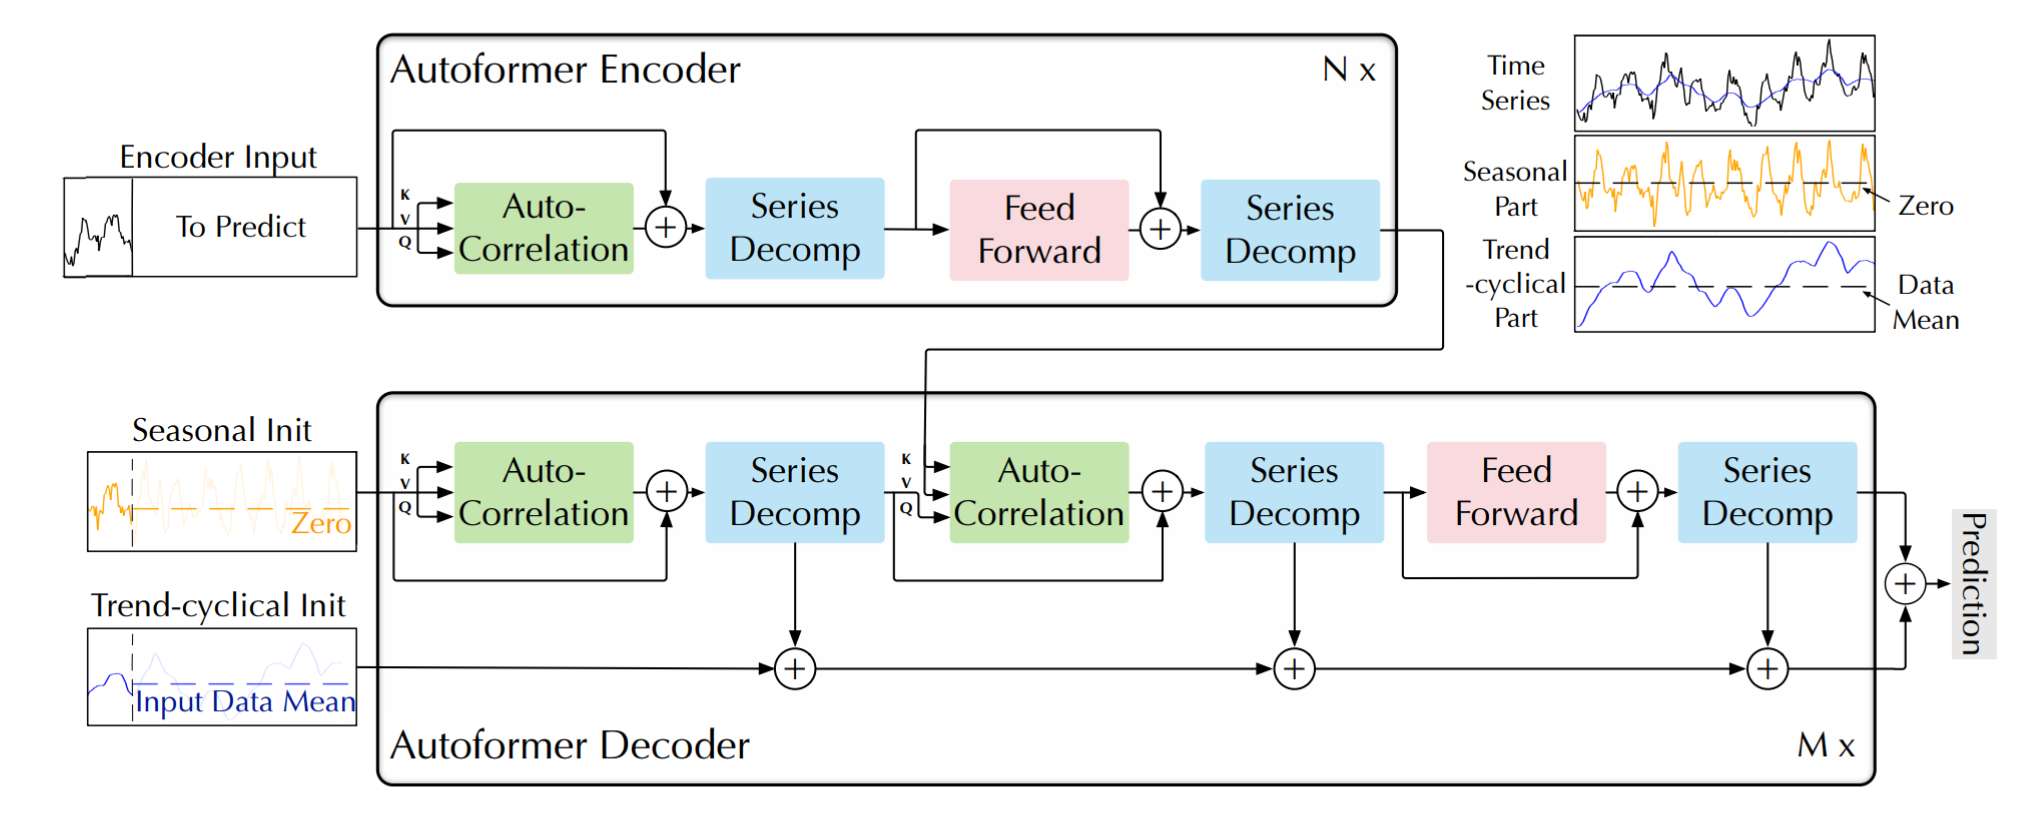
\includegraphics[scale=0.2]{img/autoformer.png}
	\caption{Autoformer: arquitectura encoder-decoder del modelo~\cite{wu2022autoformerdecompositiontransformersautocorrelation}}
	\label{autformer}
\end{figure}

A continuación, analizaremos brevemente ambas puntos diferenciales.

\paragraph{Encoder. Descomposición y autocorrelación} 
Para comprender el funcionamiento de los dos mecanismos, estudiaremos primero su funcionamiento desde el punto de vista del encoder. Este recibe la secuencia de entrada \(X^{en} \in \mathbb{R}^{L_x \times d_{\text{model}}}\) y procesa la señal mediante capas que combinan, en cada paso, una etapa de descomposición y otra de agregación basada en autocorrelación. \\

En primer lugar, se produce la descomposición progresiva, que está constituida por un bloque interno realiza suavizado local a través de mecanismos como la media móvil para extraer la componente de tendencia y obtener el residuo estacional:
\[
X_t = \operatorname{MA}_w(X), \qquad X_s = X - X_t,
\]
donde \(\operatorname{MA}_w\) es una media móvil de ventana \(w\). Al aplicar este procedimiento iterativamente, las oscilaciones lentas se capturan en \(X_t\) y las variaciones rápidas permanecen en \(X_s\), reduciendo ruido y separando dinámicas.\\

Tras la descomposición progresiva en tendencia y estacionalidad, Autoformer aplica el módulo de autocorrelación (figura \ref{autocorrelacion}) sobre la componente estacional, con el objetivo de identificar retardos (\textit{lags}) que representen dependencias temporales significativas.

\begin{figure}[!ht]
	\centering
	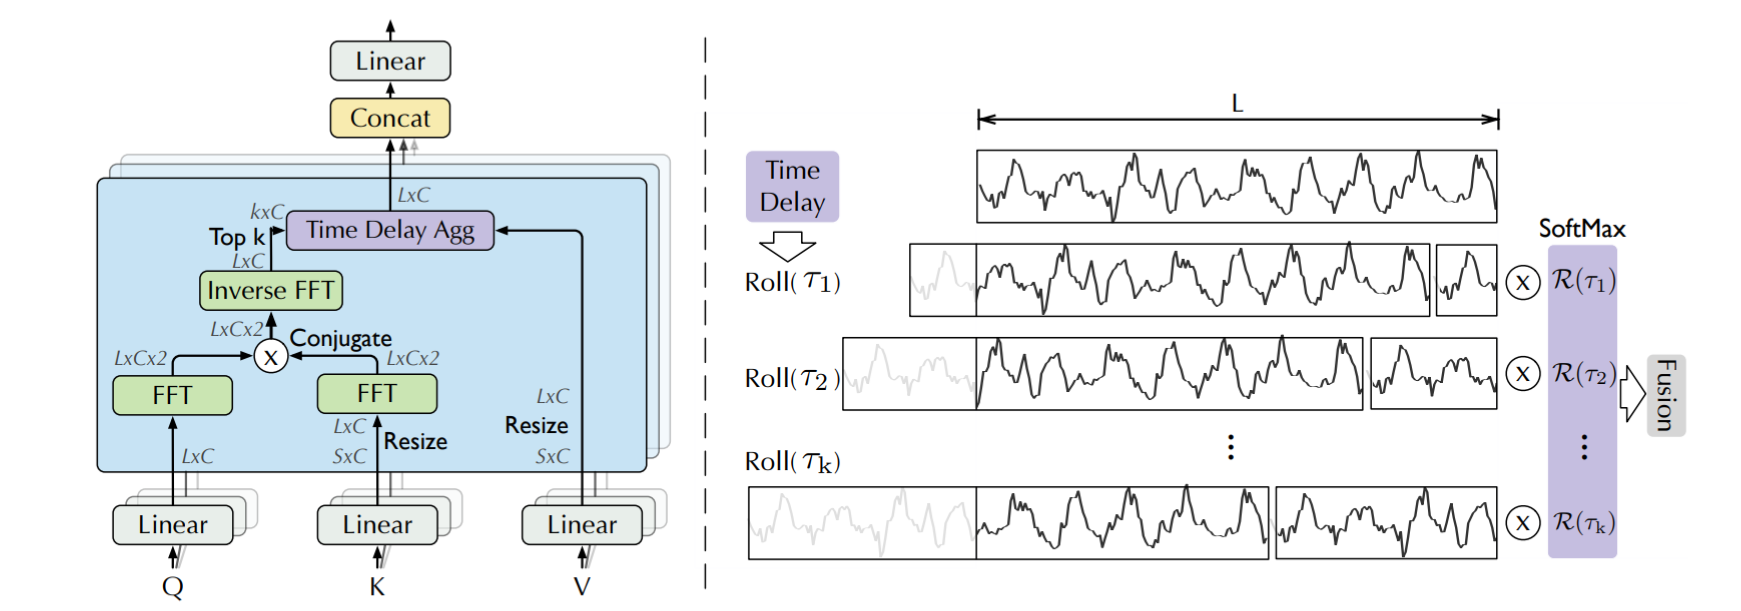
\includegraphics[scale=0.25]{img/autocorrelacion.png}
	\caption{Autoformer: cálculo de la autocorrelación empleando FFT~\cite{wu2022autoformerdecompositiontransformersautocorrelation}}
	\label{autocorrelacion}
\end{figure}

Sea $\mathbf{X} = \{x_t\}_{t=1}^L$ la secuencia de entrada, la autocorrelación se calcula como:
\begin{equation}
	R_{xx}(\tau) \;=\; \sum_{t} x_t \, x_{t+\tau},
\end{equation}
lo que en la práctica se implementa de forma eficiente mediante Transformada Rápida de Fourier (FFT) con complejidad $O(L \log L)$.

A partir de $R_{xx}(\tau)$ se selecciona el conjunto $\mathcal{T}$ de retardos con mayor magnitud, y se construye la nueva representación agregada:
\begin{equation}
	\tilde{x}_t \;=\; \frac{1}{|\mathcal{T}|} \sum_{\tau \in \mathcal{T}} w_\tau \, x_{t-\tau},
\end{equation}
donde $w_\tau$ es un peso proporcional a la magnitud de correlación.\\

A diferencia del \textit{self-attention} tradicional, que opera sobre puntos individuales, este mecanismo agrega información a nivel de subserie, reduciendo la sensibilidad al ruido y mejorando la captura de patrones periódicos de largo plazo.

\paragraph{Decoder. Alineamiento mediante Cross-Correlation} 

Una vez definido el encoder, podemos pasar a estudiar la estructura del decoder. En este módulo, se procede a realizar la inferencia de la secuencia objetivo, la cual se construye a partir de un \textit{contexto} formado por dos componentes iniciales: la tendencia inicial (\textit{trend init}) y la estacionalidad inicial (\textit{seasonal init}), otorgando al modelo así un token de contexto de forma similar a Informer. Pero a diferencia de este, no se está insertando información de entrada tal cual, sino que se está aprovechando información ya aprendida por el encoder; la tendencia inicial se obtiene extrapolando la componente de tendencia calculada en el último segmento observado por el encoder, proporcionando una base suave sobre la que se construirá la predicción. Y la estacionalidad inicial, se genera tomando el último patrón estacional estimado por el encoder. Estas dos señales conforman el punto de partida sobre el que se añadirá la información procedente de la autocorrelación cruzada.\\

El contexto completo, compuesto por estas inicializaciones y el bloque correspondiente al horizonte de predicción vacío, se proyecta al espacio de trabajo mediante las mismas proyecciones lineales y codificaciones posicionales que en el encoder, garantizando una representación homogénea.\\

Posteriormente, la representación de entrada se somete nuevamente al bloque de descomposición, separando sus componentes de tendencia y estacionalidad en cada capa. La tendencia se modela mediante extrapolación suave, mientras que la estacionalidad se reconstruye a partir de las periodicidades detectadas en la secuencia histórica procesada por el encoder. Para este proceso,  se sustituye la atención cruzada habitual por un mecanismo de cross-autocorrelation, que mide la correlación cruzada entre la estacionalidad generada en el \textit{decoder}, $s^{de}$, y la estacionalidad producida por el \textit{encoder}, $s^{en}$:
\begin{equation}
	R_{cross}(\tau) \;=\; \sum_{t} s^{de}_t \; s^{en}_{t+\tau}.
\end{equation}

De manera análoga al encoder, se emplea FFT para calcular las correlaciones con complejidad $O(L \log L)$ y se identifican los retardos $\tau$ con mayor magnitud. Con este conjunto de retardos relevantes $\mathcal{T}$, la reconstrucción de la estacionalidad en el \textit{decoder} se realiza agregando las posiciones correspondientes del \textit{encoder}:
\begin{equation}
	\tilde{s}^{de}_t \;=\; \frac{1}{|\mathcal{T}|} \sum_{\tau \in \mathcal{T}} w_\tau \; s^{en}_{t-\tau},
\end{equation}
donde $w_\tau$ pondera cada retardo según su magnitud de correlación.\\

Gracias a este procedimiento, podemos alinear de forma precisa las posiciones objetivo con los patrones recurrentes identificados en los datos históricos, y empleando dicha información para realizar forecasting pero sin incurrir en el elevado coste computacional del \textit{cross-attention} convencional.

\paragraph{Análisis crítico y conclusiones}

Las mejoras propuestas por Autoformer suponen un salto considerable sobre los métodos existentes hasta ese momento, ya que permitió mejorar considerablemente los resultados ofrecidos por Informer y el resto de Transformers más referenciados aquel tiempo~\cite{wu2022autoformerdecompositiontransformersautocorrelation}.\\

El mecanismo de descomposición, el cual puede parecer simple e intuitivo, permite al modelo centrarse en encontrar patrones ocultos más complejos dentro de la serie, y facilita el proceso de detección de patrones estacionales en una complejidad computacional equivalente a \(O(L \log L)\).\\

En cuanto a la autocorrelación, esta se trata de una de las principales ventajas. Si bien se aleja como tal de lo podría ser considerado un Transformer canónico, en el que destacó su mecanismo de atención punto a punto, emplear autocorrelación a modo de mecanismo de ordenación ha ofrecido buenos resultados experimentales en los conjuntos probados. La mejora es evidente, principalmente, frente a cualquier método de atención basado en muestreo, ya que de esta forma no estamos sometidos a la probabilidad a la hora de realizar el muestreo (ver figura \ref{muestreo}). Hemos eliminado el riesgo de suprimir puntos de gran interés dentro de la serie temporal, ya que la autocorrelación nos permite encontrar patrones de manera bastante intuitiva, recurriendo a conceptos tradicionalmente empleados en este ámbito en los modelos AR. 
	
\begin{figure}[!ht]
	\centering
	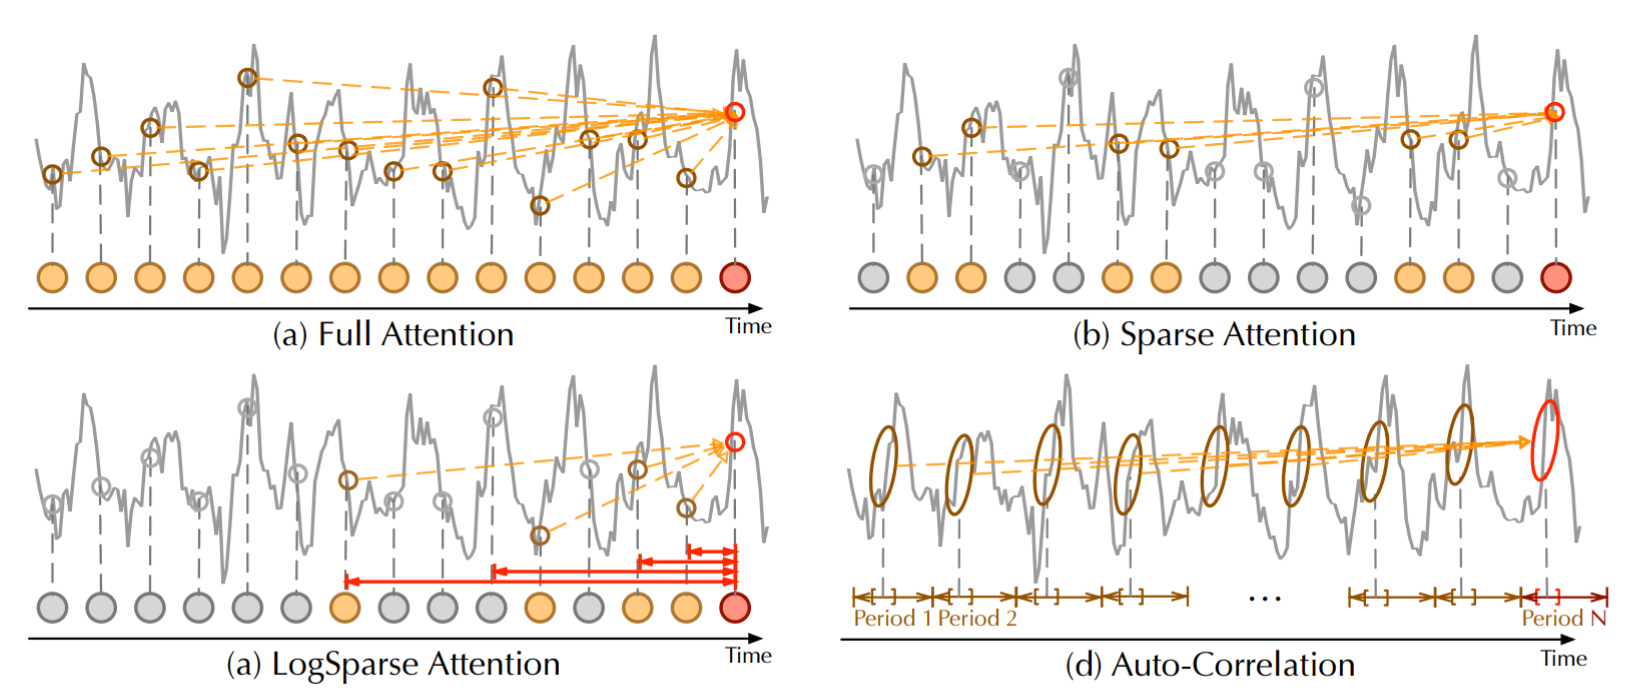
\includegraphics[scale=0.25]{img/muestreo.png}
	\caption{Autoformer: comparativa de autocorrelacion vs variantes de atención ~\cite{wu2022autoformerdecompositiontransformersautocorrelation}}
	\label{muestreo}
\end{figure}

Además, de manera implícita, estamos agregando al modelo información espacial local del conjunto de datos, ya que la autocorrelación es capaz de encontrar información como patrones estaciones y anomalías de manera más directa que los mecanismos probabilísticos de atención vistos hasta ahora.\\

Sin embargo, a modo de crítica, podemos insistir en la falta de desarrollo del positional encoding a la hora de construir el embedding. Si bien es cierto que el uso de autocorrelación mejora sensiblemente la incorporación de información local al modelo, un mejor encoding podría favorecer aún más su funcionamiento, dejando de lado el rígido encoding sinusoidal y empleando algún tipo de codificación más adaptada a los datos. Y, por último, aunque su arquitectura se asemeja bastante a un Transformer, de forma purista y matemática se aleja de lo que originalmente se definió en \textit{Attention is All You Need}~\cite{vaswani2023attentionneed} al no usarse un mecanismo de atención. Pero su arquitectura es lo suficientemente similar, teniendo a la autocorrelación como un sustituto sólido, por lo que es indiscutible que ofrece un buen rendimiento tomando una arquitectura similar.

\subsubsection{FEDformer (2022)}

Otro de los modelos que más citados que adaptan los Transformer para su uso en series temporales es FEDformer~\cite{zhou2022fedformerfrequencyenhanceddecomposed}, cuyo nombre proviene de \textit{Frequency Enhanced Decomposition Transformer}. Este modelo, al igual que Autoformer, trata de descomponer la serie temporal para ser capaz de estudiar con mayor precisión su comportamiento. Parte de algunos de los principios de este último, pero, en lugar de basarse en la descomposición típica aditiva, emplea las transformadas de Fourier y Wavelet para ir más allá del dominio temporal.\\

Para ello, propone la agregación de resultados de un modelo compuesto por caminos bien diferenciados capaces de procesar la serie siguiendo los dos enfoques propuestos. La utilidad de introducir ambos caminos se ve justificada por la necesidad de modelar la red como un procedimiento secuencia a secuencia, pero añadiendo solo los detalles con la granularidad deseada. Filtrar demasiado la red podría suprimir detalles de alta frecuencia de interés que podrían ser claves, pero realizarlo de manera demasiado detallada podría introducir ruido; así como en el caso contrario, usar solo frecuencias bajas podría crear un modelo demasiado genérico y pobre, que únicamente sirva para modelar la tendencia.\\

 Este refinamiento a nivel estructural puede conseguirse a través de Fourier, ya que permite seleccionar un número de componentes concretas a calcular para limitar el nivel de granularidad de los datos y conseguir así un nivel de precisión equilibrado.\\
 
 Por otro lado, la descomposición Wavelet nos permite realizar un análisis multiescalar de la serie, logrando asi obtener detalles estructurales de la misma a diferente nivel, y permitiendo mejorar la identificación de patrones cíclicos en los datos.\\
 
 \begin{figure}[!ht]
 	\centering
 	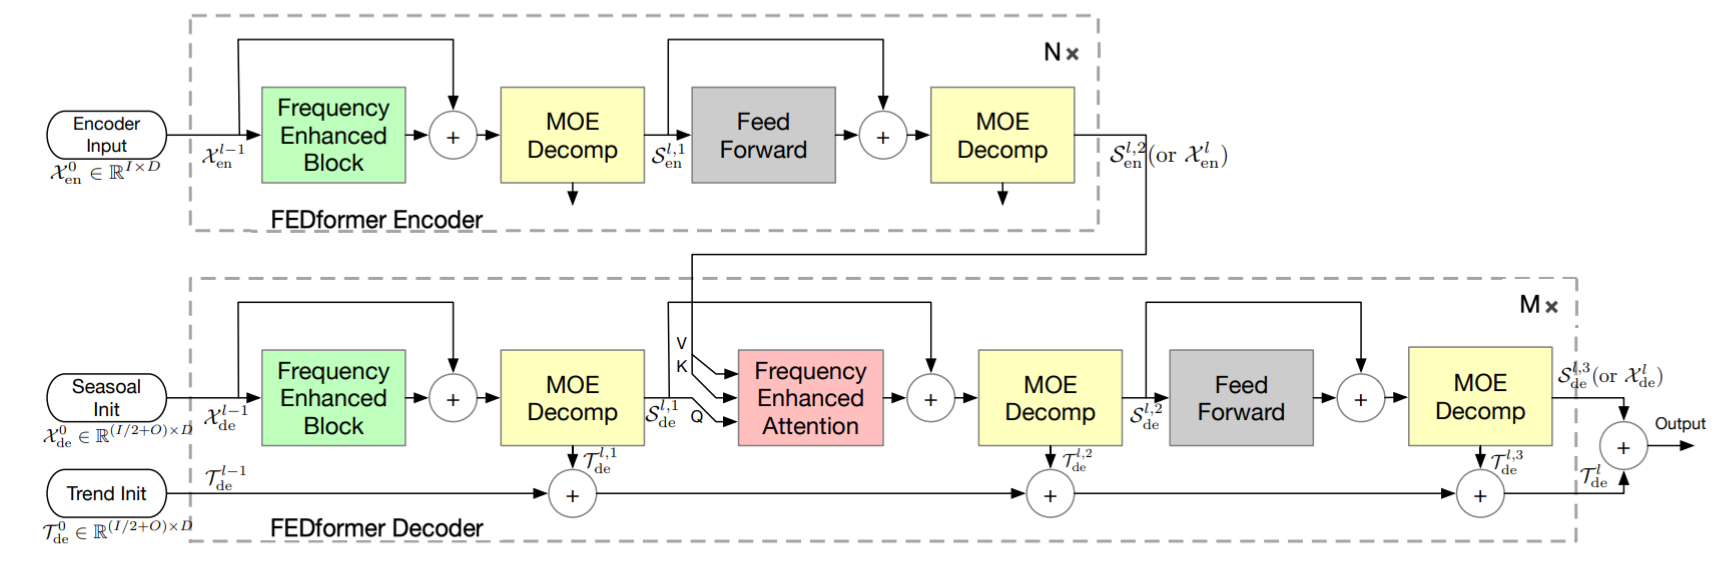
\includegraphics[scale=0.25]{img/fedformer.png}
 	\caption{FEDformer: arquitectura del modelo \cite{zhou2022fedformerfrequencyenhanceddecomposed}}
 	\label{fedformer}
 \end{figure}
 
 
 A continuación, examinaremos en mayor detalle la arquitectura, la cual incluye la incorporación de 4 nuevos módulos, sustitutos de los módulos de atención y autocorrelación, y que trabajan de manera independiente mediante Fourier y Wavelet para posteriormente combinarse para el resultado final, dando lugar a lo que sus autores consideran un procedimiento de ``hibridación de expertos''~\cite{zhou2022fedformerfrequencyenhanceddecomposed} (ver figura \ref{fedformer}).
 
 
\paragraph{Módulo Fourier}

El módulo de Fourier reemplaza parcialmente la atención tradicional, utilizando las transformadas para operar en el dominio de la frecuencia. La idea central es que muchas dependencias temporales, pero especialmente las de largo plazo, se manifiestan como componentes periódicas o cíclicas que resultan más fáciles de identificar y procesar cuando la señal se transforma mediante una {transformada de Fourier.\\

El proceso comienza aplicando la transformada discreta de Fourier (DFT) sobre la componente estacional de la serie, por lo que ya se parte de una red previamente descompuesta, al estilo de lo que vimos en Autoformer. Luego, en lugar de trabajar con todas las frecuencias, se seleccionan solo las más significativas, es decir, que posean una mayor magnitud espectral, y de esta forma, se realiza un fase de filtrado que suprime el ruido y enfoca el modelo en patrones relevantes. Se estima que, fijando un número concreto de componentes, el modelo es capaz de ejecutarse en un orden de complejidad equivalente a $O(n)$, por lo que se trata de un comportamiento más eficiente que si se seleccionan todas ellas, lo cual conllevaría $O(n^2)$.\\

Una vez seleccionadas, estas frecuencias se procesan mediante un módulo de atención espectral, que evalúa dependencias entre fases y magnitudes para identificar relaciones relevantes entre distintos momentos temporales. Finalmente, se aplica la transformada inversa para volver al dominio temporal, obteniendo una versión enriquecida y más estructurada de la serie original.\\

Para explotar esta estructura, el modelo introduce dos módulos que trabajan de manera conjunta sobre la entrada relacionados: el \textit{Frequency Enhanced Attention de Fourier} (FEA-f) y el \textit{Frequency Enhanced Block de Fourier} (FEB-f).

\begin{itemize}
	\item El módulo \textbf{FEA-f}(figura \ref{feaf}) es el encargado de transformar las representaciones estacionales al dominio espectral utilizando la transformada rápida de Fourier (FFT), seleccionando las \textit{K} frecuencias con mayor magnitud. Sobre este conjunto reducido de componentes se aplica un mecanismo de atención espectral que, en lugar de evaluar similitudes entre posiciones temporales, compara directamente las frecuencias seleccionadas. Esta atención se ejecuta sobre un número pequeño y fijo de entradas, como 64 o 128, por lo trata de acotarse así su complejidad. Tras esta operación, se deshacen los cambios de la FFT para volver al dominio temporal.
	
	 \begin{figure}[!ht]
		\centering
		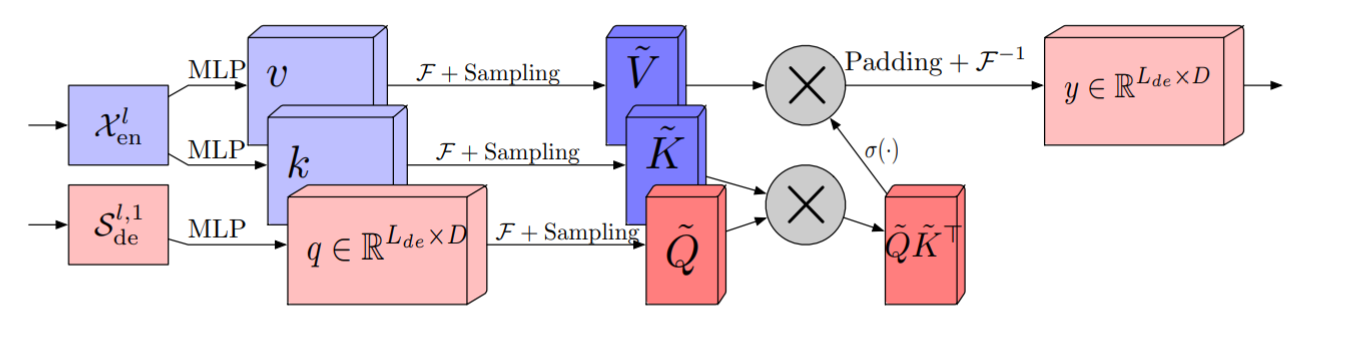
\includegraphics[scale=0.225]{img/feaf.png}
		\caption{FEDformer: arquitectura del módulo FEA-f \cite{zhou2022fedformerfrequencyenhanceddecomposed}}
		\label{feaf}
	\end{figure}
	
	\item El bloque \textbf{FEB-f} encapsula el proceso anterior dentro de una arquitectura residual completa, incorporando normalización, proyecciones lineales y conexiones residuales, y se emplea como unidad básica tanto en el encoder como en el decoder. Aunque introduce capas adicionales, su complejidad sigue dominada por el coste de la FFT y su inversa, $O(n \cdot \log{n})$, pero a pesar de ello, sigue siendo más eficiente que la atención clásica.
	
	\begin{figure}[!ht]
		\centering
		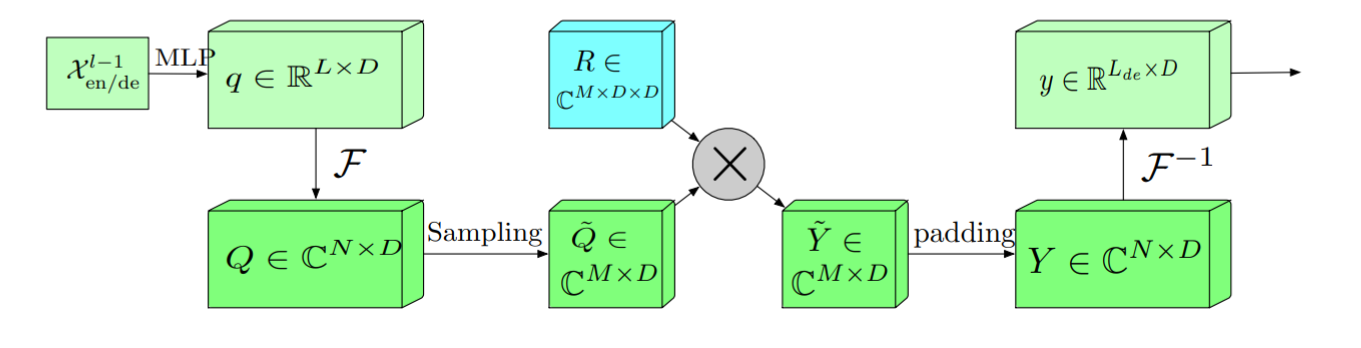
\includegraphics[scale=0.225]{img/febf.png}
		\caption{FEDformer: arquitectura del modulo FEB-f \cite{zhou2022fedformerfrequencyenhanceddecomposed}}
		\label{febf}
	\end{figure}
\end{itemize}

\paragraph{Módulo Wavelet}

El módulo basado en \textit{wavelets} busca realizar un procedimiento similar en estructura al de Fourier. Mientras que esta última se ocupa de procesar y detectar patrones estacionales a lo largo de toda la secuencia, la transformada discreta wavelet (DWT) permite descomponer la señal en distintas escalas de frecuencia conservando su localización temporal, siendo una propiedad resulta clave para modelar estructuras no estacionarias presentes en series reales.\\

Aplicando la DWT sobre la componente estacional, se obtiene una representación jerárquica que separa componentes de baja y alta frecuencia, permitiendo escoger de manera equilibrada entre ambos mediante selección de coeficientes. Al igual que en el módulo anterior, se tratarán de escoger los más informativos y se procesan mediante un mecanismo de atención adaptado, que comparará las relaciones entre escalas y fases en lugar de posiciones temporales, para finalizar reconvirtiendo al espacio temporal mediante la transformada inversa (IDWT).\\

Para articular esta lógica dentro del modelo, se adaptan los módulos FEA y FEB a su uso con Wavelet (ver figura \ref{wavelet}):

\begin{itemize}
	\item El módulo \textbf{FEA-w} (\textit{Frequency Enhanced Attention - wavelet}) se encarga de transformar la representación estacional al dominio wavelet mediante DWT, seleccionar un subconjunto reducido de coeficientes relevantes y aplicar una atención jerárquica sobre estas componentes, todo ello acotando la complejidad computacional, y la localidad temporal.
	
	\item El bloque \textbf{FEB-w} (\textit{Frequency Enhanced Block - wavelet}) encapsula el módulo FEA-w dentro de una arquitectura residual completa, integrando normalización por capas, proyecciones lineales y conexiones residuales, y se emplea tanto en el encoder como en el decoder, replicando el diseño general de la versión Fourier pero adaptado al dominio wavelet. La complejidad global del módulo viene dominada por las operaciones de DWT e IDWT, cuyo coste práctico se aproxima a $O(n)$, lo que permite escalar el modelo a horizontes largos pero con alta eficiencia computacional.
\end{itemize}

	\begin{figure}[!ht]
	\centering
	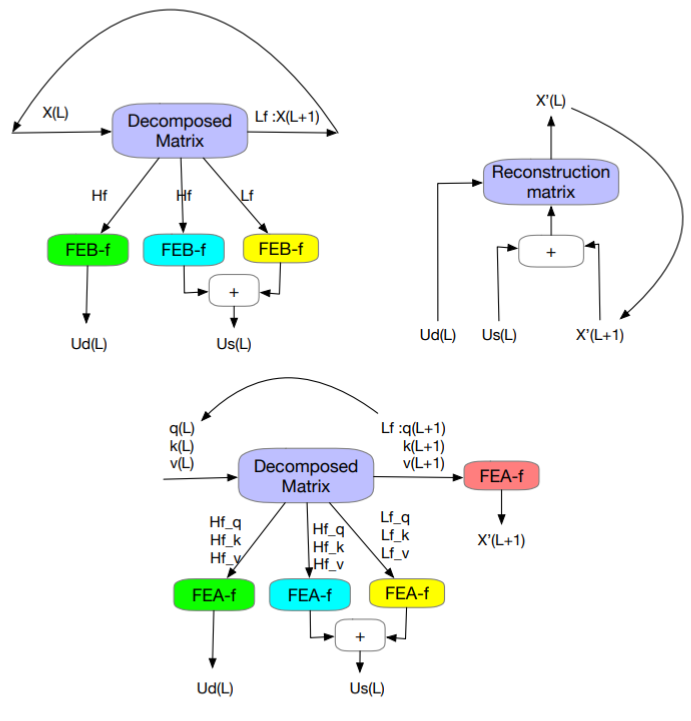
\includegraphics[scale=0.35]{img/wavelet.png}
	\caption{FEDformer: Izquieda: Etapa FEB. Arriba a la derecha: Etapa de reconstrucción de bloques de wavelets (compartida por FEB-w y FEA-w). Abajo: Etapa de descomposición de cross-attention de wavelets en el decoder. \cite{zhou2022fedformerfrequencyenhanceddecomposed}}
	\label{wavelet}
\end{figure}

\paragraph{Análisis crítico y conclusiones finales}

Tras estudiar FEDformer, hemos podido entender con mayor profundidad los cambios introducidos en la arquitectura, y su impacto con respecto a los modelos anteriores. Tomando como referencia a Autoformer para su definición, el modelo ha desarrollado mucho más el pipeline de procesado de los datos, empleando la descomposición, pero aprovechando las diferentes componentes para estudiarlas en el dominio de la frecuencia a través de Fourier y Wavelet. Los resultados obtenidos son positivos~\cite{zhou2022fedformerfrequencyenhanceddecomposed}, superando Autoformer en rendimiento para los datasets evaluados, aunque con menor diferencial al existente entre Informer y Autoformer.\\

Sin embargo, aunque apreciemos mejoras, es importante profundizar para entender realmente lo que se ha conseguido, y el impacto real. Al aplicar Fourier, realmente, estamos usando una transformación de funciones trigonométricas basadas en senos y cosenos, que de manera profunda, están bastante relacionados con la codificación ya vista en Transformer vanilla, donde se emplean como positional encoding. Por tanto, más que el propio uso de la FFT, lo que beneficia al modelo es el filtrado realizado al escoger solo el subconjunto de coeficientes más significativo, reduciendo el ruido.\\

En cuanto a la aplicación de Wavelet, nuevamente, se está aplicando cierto proceso de filtrado o suavizado al escoger un subconjunto de los coeficientes, pero en este caso, la transformación puede llegar a ser más interesante desde el punto de vista teórico, ya que se trata de buscar patrones en diferentes granularidades de la serie temporal. Pero, en el ablation study cubierto por la publicación original \cite{zhou2022fedformerfrequencyenhanceddecomposed}, los resultados son más estables numéricamente cuando se emplea la variante de Fourier, por lo que su viabilidad práctica parece limitada posiblemente a un subconjunto de casos a determinar.\\

En lo que respecta a la estructura, se vuelve a tomar una tendencia más cercana al Transformer original, ya que se recupera de nuevo el concepto de atención propiamente dicho. Y, a pesar de que el uso de caminos múltiples de aprendizaje pueda dificultar la implementación, dicho enfoque le agrega variedad y riqueza a los resultados obtenidos, por lo que podría ser una vía interesante de expansión.

\subsection{Otros modelos actuales}

En los últimos dos años, podemos encontrar nuevos modelos que siguieron alejándose dela estructura del Transformer, con el objetivo de mejorar el procesamiento de la entrada, centrándose en la descomposición por patches, o alterando el mecanismo de atención para acercarse en mayor medida a la semántica del problema:

\begin{itemize}
	\item \textbf{PatchTST} (2023)~\cite{nie2023timeseriesworth64}. Toma inspiración en los Vision Transformers, y su principal innovación consiste en representar la señal mediante \textit{patches} temporales,en lugar de procesar cada instante individualmente. Esta estrategia permite capturar contexto local de forma más eficiente y reduce la longitud efectiva de la secuencia.
	
	El modelo aplica self-attention entre parches completos, lo que favorece la detección de dependencias de largo alcance. Para preservar la información temporal se utilizan \textit{embeddings posicionales}, y en el caso de series multivariantes, se adopta una estrategia \textit{channel-independent} que procesa cada variable por separado para modelarlas.
	
	Curiosamente, prescinde de decoder, debido al uso de una capa lineal proyectada directamente desde la salida del encoder, evitando así arquitecturas y mejorando el rendimiento gracias al no operar la salida punto a punto, sino como secuencia completa.
	
	\item \textbf{TimeNet} (2023)~\cite{wu2023timesnettemporal2dvariationmodeling}. Este modelo sigue un enfoque más distante de los Transformers, a los que considera en su publicación realmente limitados para el procesado de señales multiescala o multiperiódicas.  Para ello, reemplaza la atención por operaciones convolucionales 2D aplicadas sobre una representación estructurada de la señal. Su punto de partida consiste en transformar la secuencia original en un conjunto de \textit{tensores 2D}, donde las columnas agrupan observaciones dentro de un mismo periodo (\textit{intra-period}) y las filas corresponden a fases similares a lo largo de distintos periodos (\textit{inter-period}), para así capturar explícitamente la estacionalidad. De esta forma, no solo podemos emplear arquitecturas ya conocidas como Inception, sino también eliminar todas las dependencias recurrentes, que son de las más costosas de este tipo de modelos.
	
	Para poder adaptar los datos se propone el \texttt{TimesBlock}, que realiza varias tareas. Primero, se identifican automáticamente los periodos dominantes en la serie mediante FFT; a partir de ellos, la secuencia se reorganiza en matrices que reflejan su estructura periódica, y a posteriormente, se procesan con arquitecturas convolucionales conocidas como la mencionada Inception. Finalmente, las salidas se fusionan adaptativamente en una única representación unidimensional, ponderando cada periodo según su importancia.
		
\end{itemize}

\subsection{Resumen comparativo}

Tras haber explorado algunas soluciones alternativas que vuelven a alejarse del Transformer tal y como lo conocemos, hemos finalizado la revisión de los principales modelos de procesado del estado del arte, partiendo de los algoritmos básicos y finalizando con complejas derivaciones del concepto original de atención.\\

Cada uno de estos métodos posee sus ventajas e incovenientes, y es crítico saber cuál de ellos emplear en cada caso. Los primeros modelos, como Informer, pueden ser a veces problemáticos si buscamos detalles de granularidad fina; Autoformer o FEDformer pueden funcionar mejor en ese aspecto, y facilitar la detección de patrones estacionales. Pero, por contra, se alejan un poco más de los mecanismos habitualmente usados en Transformers, y no podremos experimentar el impacto de diferentes encoding posicionales, que es el objetivo que estamos tratando. \\

A modo de resumen, se muestra la tabla \ref{resumenmodelos}, donde se pueden apreciar las diferentes características de cada modelo.

\begin{table}[H]
	\centering
	\begingroup
	\renewcommand{\arraystretch}{1.15}
	\begin{tabular}{P{2.25cm} | P{2cm} P{2cm} P{3cm} P{3.2cm}}
		\toprule
		\textbf{Modelo} & \textbf{Positional Encoding} & \textbf{¿Captura periodicidad?} & \textbf{Mecanismo principal} & \textbf{Uso destacado} \\
		\midrule
		Transformer & Sinusoidal / Aprendido  & Limitado & Atención completa & Modelo base, generalista para secuencias \\
		Transformer-XL & Aprendido relativo & No explícitamente & Atención recursiva con segmentación & Maneja dependencias a muy largo plazo con estado recurrente \\
		Reformer & Sinusoidal  & No explícitamente & Atención local + hashing & Escalabilidad para secuencias muy largas \\
		LogTrans & Sinusoidal & No explícitamente & Atención logarítmica & Mejor manejo de dependencias a largo plazo \\
		Informer & Sinusoidal  & No explícitamente & Atención ProbSparse & Eficiencia computacional para secuencias largas \\
		Autoformer & Implícito (autocorrelación)  & Sí & Autocorrelación & Captura explícita de patrones periódicos \\
		FEDformer & Implícito (FFT)  & Sí & Atención + FFT & Buena capacidad de captura de patrones y eficiencia \\
		\bottomrule
	\end{tabular}
	\caption{Comparativa entre modelos Transformer para series temporales}
	\label{resumenmodelos}
	\endgroup
\end{table}

Tal y como ya adelantábamos en los análisis realizados tras estudiar cada modelo, podemos ver que la codificación posicional ha sido un aspecto no especialmente atendido en la formulación de cada modelo. Si bien modelos como Autoformer y FEDformer tratan de compensar esto mediante sus propios mecanismos de atención o equivalentes más elaborados, la construcción del embedding permanece igual a prácticamente como se realizaba en los Transformer vanilla. Por tanto, esto justifica y muestra la necesidad de probar una nueva vía de investigación que trate de verificar si, incluso empleando modelos de aprendizaje más sencillos, como lo es el Transformer original o Informer, se pueden obtener buenos resultados de por sí trabajando con la codificación posicional.\\

En el próximo capítulo, nos centraremos en el contexto teórico que rodea este concepto, analizando en detalle las propuestas más recientes aplicadas a series temporales \cite{irani2025positionalencodingtransformerbasedtime}, y a partir de ello, formularemos y compararemos distintas variantes, con el objetivo de extraer conclusiones relevantes sobre su eficacia y aplicabilidad.

\chapter{Estudio teórico. Propuestas en Positional Encoding}

En el capítulo anterior, presentamos los principales modelos de aprendizaje para series temporales, y así analizar las soluciones propuestas por cada uno. Al hacerlo, pudimos identificar un problema clave: la codificación posicional no recibe la atención necesaria, y en la mayoría de casos se usa la formulación original, con adaptaciones mínimas, o bien, es suprimido a favor de otras alternativas incorporadas en la propia arquitectura.\\

En este capítulo, teniendo presente los tipos anteriormente descritos de codificaciones (fijo, aprendible, adición de variables temporales, transformaciones), retomaremos esa clasificación para profundizar en las propuestas más recientes orientadas específicamente a series temporales, analizando su motivación, diseño y posibles ventajas frente a las formulaciones clásicas.\\

Partiremos del esquema tradicional de codificación posicional heredado del Transformer original y examinaremos cómo distintos trabajos recientes han intentado superar sus limitaciones mediante adaptaciones de carácter local o dependientes del contenido. Nuestro objetivo será identificar las ventajas concretas que aporta cada enfoque, extraer de ellos la inspiración necesaria y, a partir de ahí, diseñar nuevos experimentos de codificación posicional que integren ideas capaces de mejorar el rendimiento del modelo.

\section{Análisis de propuestas existentes}

Durante el análisis de los modelos más destacados del estado del arte, hemos podido ver en uso, principalmente, el mecanismo tradicional de atención basado en senos y cosenos, así como el basado en las transformadas de Fourier y Wavelet, en el caso de FEDformer. Sin embargo, dejando al margen estos enfoques, no hemos apreciado ninguna otra alternativa intuitiva que trate de mejorar el positional encoding más allá, ya que en otros casos, directamente se opta por su supresión o compensación por otro mecanismo.\\

Para poder profundizar más en este aspecto, podemos adentrarnos en surveys como el publicado por \textit{Habib Irani y Vangelis Metsis}~\cite{irani2025positionalencodingtransformerbasedtime}, donde se recogen multitud de variantes de encoding, aplicados a series temporales. Tomando como referencia la clasificación propuesta (ver figura \ref{encodings}), a continuación agruparemos las codificaciones posicionales en dos grandes categorías. Por un lado, aquellas que se incorporan sumándose directamente al embedding de entrada, conocidas como métodos absolutos de codificación posicional (APE); por otro, las que actúan modificando el propio cálculo de la atención, y que por ello se denominan métodos relativos de codificación posicional (RPE).


\begin{figure}[!ht]
	\centering
	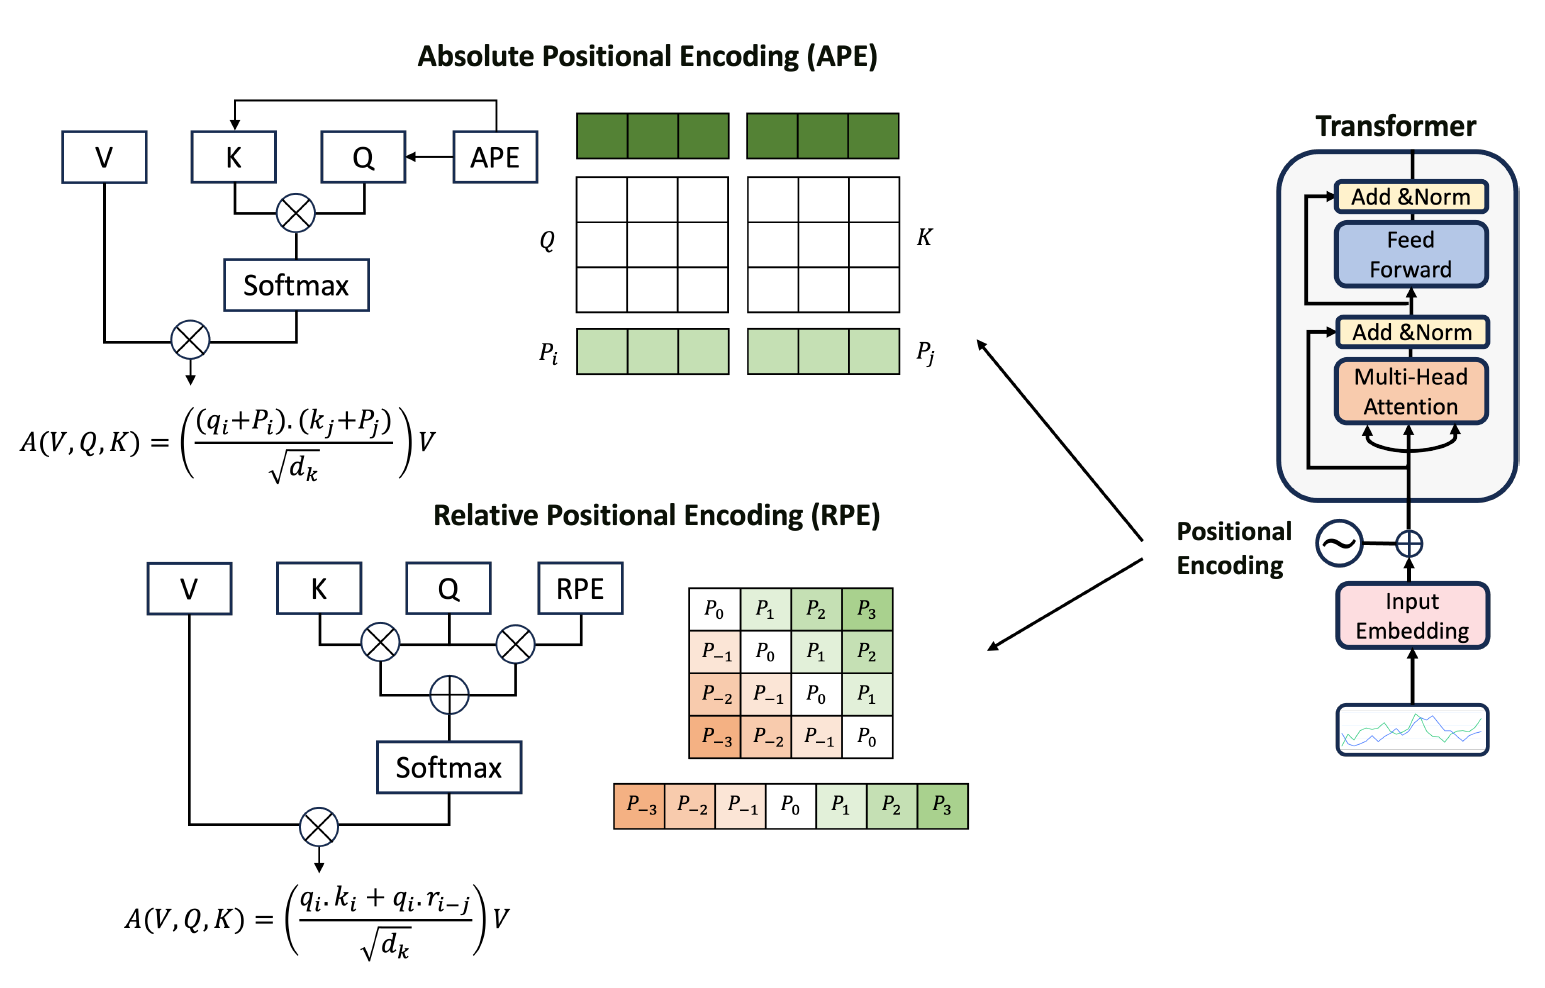
\includegraphics[scale=0.275]{img/encodings.png}
	\caption{Encodings: clasificación de métodos y funcionamiento \cite{irani2025positionalencodingtransformerbasedtime}}
	\label{encodings}
\end{figure}

\subsection{Métodos aditivos}

Comenzaremos el análisis por el positional encoding aditivo. Esta vertiente toma como referencia el mecanismo de adición de información empleado por el enfoque sinusoidal original, ya que todas estas codificaciones se añaden al embedding mediante suma, de forma que no es necesario realizar modificaciones adicionales a la arquitectura neural que los procesará, y facilita el uso de modelos preentrenados con el fin de ahorrar recursos de cómputo.\\

En mayor detalle, estos métodos construyen un vector posicional $(P \in \mathbb{R}^{L \times d})$ y lo se suma directamente a los embeddings de entrada (X), obteniendo:

$$ X' = X + P $$

donde (L) es la longitud de la secuencia y (d) la dimensión del embedding.\\

Suponen una ventaja desde el punto de vista de la usabilidad, ya que modificar excesivamente los mecanismos de atención puede dificultar su comprensión y provocar efectos adversos indeseados si no se realiza con el rigor necesario. A continuación, destacaremos algunos de los mecanismos existentes con estas características, y analizaremos la utilidad ofrecida por cada uno.

\subsubsection{Sinusoidal Positional Encoding (PE)}

Se trata del encoding original propuesto originalmente por Vaswani et al. (2017)~\cite{vaswani2023attentionneed}, a modo de recordatorio. Como ya vimos, utiliza funciones sinusoidales para representar la posición:

$$
PE_{(pos, 2i)} = \sin\left(\frac{pos}{10000^{\frac{2i}{d}}}\right)
$$

$$
PE_{(pos, 2i+1)} = \cos\left(\frac{pos}{10000^{\frac{2i}{d}}}\right)
$$

Donde cada variable indica:

\begin{itemize}
	\item \textbf{pos}: índice temporal (posición).
	\item \textbf{i}: dimensión del componente del embedding.
	\item \textbf{d}: dimensión total del embedding.
\end{itemize}

Basándonos simplemente en su formulación, fuimos capaces de distinguir ya sus ventajas y desventajas; como ventaja, podemos ver que se trata de una codificación no entrenable, por lo que para unas mismas dimensiones de entrada de datos, el resultado será siempre el mismo, y sus valores no se deben entrenar época a época de manera independiente. Esto lo hace más sencillo de usar, y más eficiente al no requerir parámetros adicionales. Sin embargo, como principal desventaja, estimamos que no permite modelar con suficiente adaptabilidad los períodos no estacionales de datos o con mayor número de irregularidades y valores anómalos.\\

Su forma sencilla de acoplar al conjunto de datos de entrada nos sirve de inspiración para la creación de nuevas variantes que traten de incorporar más contexto semántico de los datos.

\subsubsection{Time Absolute Positional Encoding (tAPE)}

tAPE propone una solución que, aunque sigue perteneciendo a la familia de codificaciones fijas, incorpora información estructural propia de la secuencia de entrada, en particular su longitud real $L$. La idea central es ajustar la escala de las frecuencias empleadas en la codificación sinusoidal en función de esa longitud, de forma que la representación posicional conserve una propiedad conocida como \textit{distance-awareness}.\\

Por \textit{distance-awareness} entendemos la capacidad de la codificación para reflejar, de manera coherente y diferenciada, la distancia relativa entre posiciones, y así complementar a la información global. En una codificación con buena distance-awareness, dos posiciones cercanas deben tener representaciones más similares entre sí que respecto a posiciones muy alejadas, y esta relación se mantiene de forma proporcional a lo largo de toda la secuencia. Es algo que no logramos cosneguir en codificaciones sinusoidales estándar, sobre todo cuando la dimensión del embedding es baja, ya que las frecuencias asignadas no siempre proporcionan suficiente resolución para representar distancias cortas.\\

Para mitigar este problema, tAPE redefine las frecuencias como:

\begin{equation}
	\centering
	\omega^{new}_k = k \cdot \frac{d_{model}}{L}
\end{equation}

Adaptando así su espectro al tamaño real de la secuencia y adecuándose incluso a casos de entrada de corta longitud. Esta nueva frecuencia simplemente se incorpora como parámetro a la codificación sinusoidal estándar:

\begin{equation}
	\begin{aligned}
		\text{PE}_{(pos,2i)} &= \sin\!\left( pos \cdot \omega^{new}_i \right) \\
		\text{PE}_{(pos,2i+1)} &= \cos\!\left( pos \cdot \omega^{new}_i \right)
	\end{aligned}
\end{equation}


Donde:

\begin{itemize}
	\item \textit{d} representa la dimensión del embedding utilizada por el modelo Transformer; este valor determina el número de componentes de la codificación posicional y, por tanto, el rango de frecuencias disponibles para representar las posiciones.
	\item \textit{L} corresponde a la longitud real de la secuencia.
	\item \textit{k} es el índice de la dimensión o de la frecuencia dentro del embedding; al recorrer k desde valores bajos a altos, obtenemos frecuencias cada vez más elevadas en las funciones seno y coseno, lo que permite representar tanto variaciones lentas (baja frecuencia) como rápidas (alta frecuencia) a lo largo de la secuencia.
\end{itemize} 

La principal virtud de tAPE es su capacidad para mantener la distance-awareness incluso en contextos con embeddings de baja dimensión, algo que no siempre se logra con la codificación sinusoidal estándar. Al incorporar la longitud real \textit{L} en el cálculo de las frecuencias, se evita que la escala sea excesivamente grande o pequeña para la secuencia procesada, lo que redunda en una representación posicional más ajustada y fiel a las distancias relativas. Esta adaptación es especialmente útil en series temporales de corta o media duración, donde las relaciones locales y su correcta discriminación son fundamentales.\\

Sin embargo, sigue teniendo limitaciones evidentes. Para empezar, su dependencia explícita de \textit{L} puede suponer un problema si, durante la inferencia, trabajamos con secuencias de longitud muy distinta a la usada en el entrenamiento, aunque normalmente, se deberían seguir distribuciones similares. Además, tAPE es un método de codificación fijo y no incorpora parámetros aprendibles, lo que si bien simplifica su uso y evita sobreajuste, también le impide adaptarse dinámicamente a patrones posicionales más complejos o irregulares presentes en diferentes dominios o conjuntos de datos.

\subsubsection{Learnable Positional Encoding (LPE)}

En el método sinusoidal tradicional, la codificación posicional se realizaba de forma fija e invariante, dependiendo únicamente de las dimensiones de los datos de entrada. Sin embargo, esto no favorece a la localización de estructuras y detalles propios de los datos de entrada, por lo que surge así el encoding posicional aprendible. Su filosofía se basa en dejar que el modelo sea quien entrene los valores de la codificación posicional a la vez que el resto de la arquitectura se refina:

$$
PE_{\text{learnable}}(pos) = W_{pos}, \quad W_{pos} \in \mathbb{R}^d
$$

Esta codificación aprendida se incorpora al embedding de entrada de manera aditiva como hasta ahora:


$$
X' = X + PE_{\text{learnable}}[pos]
$$

La principal fortaleza de este método reside en su capacidad de adaptación. A diferencia de métodos como el PE sinusoidal o tAPE, que imponen un patrón posicional fijo, LPE permite que el modelo aprenda directamente, a partir de los datos, la representación posicional que mejor captura las relaciones temporales y estructurales relevantes para la tarea. Esta flexibilidad puede traducirse en una mayor precisión, especialmente en dominios donde las dependencias posicionales no siguen un patrón excesivamente regular, o cuando la información contextual es altamente específica del conjunto de datos y es compleja de detectar de manera intuitiva.\\

No obstante, esta flexibilidad tiene un precio. Al añadir un vector de parámetros por cada posición, el tamaño del modelo crece linealmente dependiendo del parámetro de longitud \textit{L}, lo que incrementa tanto el coste de almacenamiento como el de entrenamiento. Además, la codificación aprendida queda estrechamente ligada al conjunto de datos utilizado para ajustarla; esto implica que, ante un cambio de dominio o de distribución de las secuencias, incluso si la longitud se mantiene, es necesario volver a entrenar los embeddings posicionales desde cero para preservar su utilidad. En contraste con tAPE, que conserva su aplicabilidad en distintos contextos gracias a su formulación fija, LPE sacrifica generalidad en favor de especialización.


\subsubsection{Temporal Positional Encoding (T-PE)}

Por último, nos centraremos en el encoding posicional temporal (T-PE), un enfoque híbrido que combina información posicional global y dependiente del contenido para enriquecer la representación. Por un lado, emplea la codificación geométrica sinusoidal clásica para la parte absoluta, para dotar al modelo de información posicional estable y determinista. Por otro lado, T-PE integra una componente semántica basada en similitud entre embeddings de los datos, que añade un sesgo contextual para capturar relaciones entre posiciones no solo por su índice temporal, sino también por su contenido o características. Esto se consigue mediante una función de suavizado gaussiano que mide la proximidad en el espacio de características entre cada par de posiciones. De esta forma, aportamos la visión semántica, elemento que principalmente queda infrarrepresentado en modelos fijos.\\

Formalmente, el modelo basa su componente geométrica mediante:

\begin{equation}
	PE_{i, 2k} = \sin\left(\frac{i}{10000^{\frac{2k}{d}}}\right), \quad
	PE_{i, 2k+1} = \cos\left(\frac{i}{10000^{\frac{2k}{d}}}\right)
\end{equation}

Y la componente semántica, que mide la similitud local entre embeddings, se define como:

$$S(i, j) = \exp\left( -\frac{\|x_i - x_j\|^2}{2\sigma^2} \right)$$

Añadiéndose al encoding final de manera aditiva:

$$T\text{-}PE(i) = PE(i) + S(i, j)$$


La principal fortaleza de este enfoque, por tanto, radica en la combinación de un anclaje posicional absoluto con una componente semántica adaptativa, lo que le permite capturar, de forma natural y simultánea, tanto las relaciones temporales globales como las similitudes entre elementos, integrando información global y local en una única representación.\\

Pero su implementación puede inducir problemas para la escalabilidad. La gaussiana entre todas las posiciones implica un coste cuadrático $O(L^2)$.- Además, su rendimiento está fuertemente condicionado por el grado de integración entre las dos componentes, ya que un desbalance podría anular las ventajas buscadas.\\

En resumen, T-PE propone un enfoque híbrido bastante interesante, capaz de emplear las ventajas del contenido estructural y el semántico.


\subsection{Métodos que manipulan la atención}

Hasta ahora, hemos explorado tres métodos de codificación posicional que comparten un rasgo común: todos operan mediante una simple suma dentro del embedding de entrada. Sin embargo, existe otra vía para mejorar el desempeño de los modelos Transformer que va más allá de la manipulación directa del embedding: intervenir directamente en el mecanismo de atención.\\

Hasta el momento, las modificaciones de atención que hemos visto se basaban principalmente en técnicas de muestreo para reducir el tamaño del producto, seleccionando un subconjunto de productos en lugar de trabajar con la matriz completa. Aunque estas estrategias mejoran la eficiencia, en esencia mantienen el mismo trasfondo matemático. Para avanzar más allá, podemos especializar el cálculo de la atención para que incorpore de manera explícita la estructura propia de las series temporales. De este modo, es en el propio proceso de atención, y durante la fase de creación del embedding, donde el modelo puede captar de manera más efectiva las dependencias temporales y las características relevantes del dominio, potenciando así su capacidad de predicción a largo plazo. A continuación, examinaremos algunos de los métodos propuestos y su funcionamiento

\subsubsection{Relative Positional Encoding (RPE)}


Una de las principales limitaciones del encoding posicional absoluto es que se basa en posiciones fijas e independientes, sin considerar cómo se relacionan entre sí los elementos en la secuencia. Mediante esta propuesta, el RPE, mejoramos el mecanismo de atención incorporando explícitamente un término que depende de la \emph{posición relativa} entre elementos, en lugar de usar solo sus posiciones absolutas.\\

Esta característica permite que el modelo capture relaciones y patrones que se mantienen constantes sin importar el punto exacto en la secuencia donde ocurren, haciendo que la atención sea más flexible y adaptativa. Desde un punto de vista matemático, la energía de atención entre los elementos en las posiciones \(i\) y \(j\) se calcula como:


\[
e_{ij} = \frac{(x_i W_Q)(x_j W_K)^\top}{\sqrt{d_z}} + \frac{(x_i W_Q)(a^K_{ij})^\top}{\sqrt{d_z}}, \quad \text{donde} \quad a^K_{ij} = W^r_K r_{i-j}
\]

Aquí, \(r_{i-j}\) representa un embedding que codifica la distancia relativa entre las posiciones \(i\) y \(j\). Las matrices \(W_Q\) y \(W_K\) son las matrices de proyección aprendibles para las queries y las keys, respectivamente, mientras que \(W^r_K\) es la proyección asociada a los embeddings relativos. El término \(d_z\) corresponde a la dimensión de las representaciones en la atención.\\

Este enfoque permite capturar relaciones relativas invariantes a traslaciones en la secuencia, lo cual resulta especialmente beneficioso para tareas en las que la distancia entre elementos es más importante que su posición absoluta. Por ello, mejora la capacidad de generalización del modelo frente a variaciones en la posición, y es especialmente útil en problemas de predicción, o clasificación, que poseen longitudes de secuencia variables.\\

Sin embargo, esta mejora tiene un coste: se incrementa tanto la complejidad computacional como el consumo de memoria, manteniéndose en orden \(O(L^2)\). Además, la implementación requiere almacenar y gestionar tablas de embeddings relativos para todas las posibles distancias, lo que puede complicar enormemente su escalabilidad en secuencias de larga duración.


\subsubsection{Efficient Relative Positional Encoding (eRPE)}

El modelo RPE anteriormente muestra una gran utilidad en series cambiantes, pero su eficiencia computacional costosa podría ser una gran limitación de uso. Por ello, existe una variante llamada eRPE, donde el sesgo relativo de las posiciones se incorpora después de aplicar la función Softmax en el cálculo de la atención. Es decir, en lugar de modificar la energía de atención antes de la normalización, el ajuste relativo se añade directamente sobre la distribución de atención ya calculada.

Formalmente, la atención sobre el elemento en la posición \(i\) se define como:

\[
\alpha_i = \sum_{j \in L} \left( \frac{\exp(e_{i,j})}{\sum_{k \in L} \exp(e_{i,k})} Ai,j + w_{i-j} \right) x_j
\]

donde \(w_{i-j}\) es un vector aprendible de  tamaño $2L - 1$. Dicho elemento es agregado tras realizar el proceso de atención, fuera de la Softmax. Así, la atención puede ajustarse localmente para enfatizar o atenuar ciertas posiciones relativas sin distorsionar la distribución global.\\

 Si bien dicha delimitación de tamaño de \textit{w} puede mejorar considerablemente el uso de memoria, acentúa la importancia de la información poisicional del embedding, por lo que se especializa su uso principalmente para tareas de clasificación, que se desvía de nuestro actual propósito de forecasting.

\subsubsection{Transformer with Untied Positional Encoding (TUPE)}

El modelo TUPE propone una formulación diferente a la vista hasta el momento con RPE: separa explícitamente la información de contenido y la información posicional durante el cálculo de la atención, evitando que ambas se mezclen o interfieran entre sí.\\

Matemáticamente, la atención entre los elementos en las posiciones \(i\) y \(j\) se calcula como la suma de dos términos:

\begin{equation}
	\alpha_{ij} = \frac{1}{\sqrt{2d}} (x_i^l W^{Q,l})\cdot(x_j^l W^{K,l})^T + \mathrm{reset}_\theta(\beta_{ij}, i, j)
\end{equation}

\begin{equation}
	\beta_{ij} = \frac{1}{\sqrt{2d}} (p_i U_Q)(p_j U_K)^T
\end{equation}

Donde $\beta_{ij}$ representa las interacciones entre posiciones; \(x_i\) representa el embedding de contenido en la posición \(i\), mientras que \(p_i\) es el embedding posicional correspondiente.\\

Esta separación evita la interferencia entre los patrones de contenido y los posicionales, permitiendo que cada componente se aprenda de forma independiente. Para datos de series temporales, esto resulta especialmente útil, ya que permite al modelo capturar tanto los patrones temporales (a través de las correlaciones posicionales) como las relaciones entre características (a través de las correlaciones de contenido) sin que ambos se interfieran mutuamente.\\

Debemos tener especial cuidado al usar este método en conjuntos de datos pequeños, ya que su mayor cantidad de parámetros puede suponer fácilmente problemas de sobreaprendizaje, los cuales tendremos que gestionar.


\subsubsection{Convolutional Stochastic Positional Encoding (Conv-SPE)}

Para cerrar el grupo de métodos que modifican la atención, tenemos Conv-SPE. Como indica su nombre, en lugar de usar codificaciones fijas o vectores aprendibles asociados a posiciones, utiliza convoluciones para capturar patrones locales y dependencias espaciales en la codificación posicional. Este enfoque se proponer a priori por ser más flexible y adaptativo, permitiendo modelar relaciones complejas a distintas escalas, incorporando un sesgo inductivo beneficioso para series temporales y mejorando la eficiencia y robustez en la captura de dependencias posicionales. \\

Su formulación comienza generando una matriz aleatoria \( Z_d \in \mathbb{R}^{M \times R} \) cuyos elementos siguen una distribución gaussiana estándar independiente e idénticamente distribuida (i.i.d.). Sobre esta matriz, se aplican filtros convolucionales aprendibles \(\Phi^Q\) y \(\Phi^K\) para transformar la información posicional en representaciones útiles para la atención:

\begin{equation}
Q_d = Z_d \otimes \Phi^Q, \quad K_d = Z_d \otimes \Phi^K
\end{equation}

Aquí, \(\otimes\) denota la operación de convolución, que consiste en aplicar un filtro móvil que recorre la matriz \(Z_d\) para extraer características locales, y \(\Phi^Q, \Phi^K\) son esos filtros que el modelo aprende durante el entrenamiento.\\

La clave de este método es que la operación de convolución, al ser local por naturaleza, captura patrones y relaciones cercanas dentro de los datos, otorgando así una estructura inductiva que se adapta a las dependencias temporales y espaciales presentes en las series temporales.\\

Además, cuando el parámetro \(R\) es suficientemente grande, la matriz resultante de estas convoluciones tiene una estructura de varianza cruzada que se aproxima al kernel de atención tradicional. Esto permite que la atención se pueda estimar de manera eficiente mediante el producto:

\begin{equation}
	P_d \approx \frac{\bar{Q}_d \bar{K}_d^T}{R}
\end{equation}

donde \(\bar{Q}_d\) y \(\bar{K}_d\) son las representaciones convolucionales normalizadas.\\

Sobre el papel, presenta varias ventajas. En primer lugar, captura relaciones relativas sin requerir atención cuadrática, gracias a la estimación realizada que es de orden lineal, facilitando su escalabilidad. Además, es más robusta ante sobreajuste por su componente estocástico. Sin embargo, aunque en principio pueda parecer más eficiente, modificar el mecanismo de atención puede ser delicado y su rendimiento depende mucho del conjunto de datos utilizado. De hecho, sus creadores señalan que este enfoque es más adecuado para tareas de clasificación de series temporales que para tareas de predicción, por lo que su aplicabilidad se aleja del contexto de este trabajo.

\section{Propuestas}
\subsection{Criterios de partida}
\subsection{PE basado en ventana de estadísticos}
\subsection{PE basado en ventana de estadísticos y lags}
\subsection{PE combinado flexible}
\subsection{PE combinado con TPE}
\subsection{PE combinado con SPE}




\chapter{Selección y Estudio de los conjuntos de datos}

En el anterior capítulo, hemos revisado el estado actual de los encodings en los modelos de series temporales, y hemos realizado cinco propuestas teniendo como principal concepto el uso de ventana para aumentar el contexto explícito de los datos, y la hibridación de diferentes métodos vistos mediante el uso de encodings ponderados. Pero con la formulación no es suficiente, ya que debemos comprobar su efectividad de manera empírica, realizando para ello diversos experimentos sobre diferentes conjuntos de datos.\\

Por tanto, en este apartado, introduciremos los diferentes conjuntos de datos seleccionados, analizando su contexto de extracción y algunas características básicas. Debido a su extenso tamaño, resulta complejo y costoso realizar representaciones gráficas sobre los datos, por lo que sólo se realizarán cuando sea posible por su extensión.

\section{Electricity Transformer Dataset (ETT)}

Este conjunto de datos fue empleado en la publicación original de Informer~\cite{zhou2021informerefficienttransformerlong}, y a raíz de su utilización, multitud de modelos posteriores han hecho uso de este dataset, a modo de conjunto de referencia para la comparativa entre arquitecturas y sus variantes. Contiene información acerca de dos transformadores eléctricos, que se encuentran en diferentes subestaciones, y se recogen datos acerca de su carga y la temperatura del aceite en el cual se encuentran sumergidos los componentes para mejorar el aislamiento.\\

Como ya mencionamos en la introducción, disponer de una buena estimación de la carga eléctrica necesaria para abastecer a una región y controlar la salud de los diferentes componentes del sistema para evitar caídas es clave para el aprovechamiento de recursos. Pero las condiciones y necesidades en cada instante pueden ser diferentes; la demanda puede verse afectada por el día de la semana, la existencia de vacaciones, estaciones del año, climatología, temperaturas... Todas ellas afectan de manera directa a las necesidades y a la eficiencia del sistema, por lo que la complejidad del problema hace que en muchas ocasiones las decisiones se tomen teniendo al alza, sobreproduciendo y sobredimensionando las necesidades para evitar problemas de abastecimiento. Sin embargo, esto no es eficiente, ya que se están desaprovechando recursos tanto en la producción de energía, en caso de usar fuentes no renovables, y en la producción e instalación de equipos.\\

Si conseguimos buenos resultados de predicción, podríamos idealmente reducir los recursos pero mantener un sistema estable. Y una componente clave de este ecuación es supervisar el estado del sistema, y en este dataset, concretamente, de los transformadores. La variable temperatura de aceite, que a priori parecía no demasiado útil, es clave en este conjunto de datos para detectar posibles anomalías que puedieran provocar un mal funcionamiento o problemas de suministro de manera bastante directa, ya que las temperaturas extremas afectan negativamente a su rendimiento. Bajo esta justificación, los autores extrajeron el conjunto de datos proveniendo de dos transformadores, y que recogen 2 años de datos minuto a minutogracias a una plataforma de recolección realizada con la colaboración de \textit{Beijing Guowang Fuda Science \& Technology Development Company}.\\

Originalmente, fueron extraídas más series de más transformadores, pero sólo se hicieron públicos dos, agrupados en la variante ETT-Small, que podemos encontrar en su correspondiente repositorio de GitHub~\cite{zhou2021etdataset}. Los datos provienen de dos regiones de una provincia de China, denominadas ETT-small-m1 y ETT-small-m2. En total, los dos años se traduce 70.080 puntos de datos por cada transformador. Adicionalmente, podemos encontrar dos variantes preprocesadas para realizar el forecasting hora a hora, reduciendo así el esfuerzo de cómputo necesario. Siguiendo la misma estructura de notación que los anteriores, reciben los nombres ETT-small-h1 y ETT-small-h2, siendo la h el indicativo de ``horario''.\\

Cada instante de los datos consta de 8 características, incluyendo el timestamp y 7 variables diferentes, entre la que se encuentra la temperatura del aceite:

\begin{itemize}
	\item \textbf{date}: Fecha y hora exacta en la que se realizó la medición, permitiendo situar cada registro en la secuencia temporal.
	
	\item \textbf{HUFL} (\textit{High Useful Load}): Componente útil de la carga cuando el transformador trabaja a un nivel alto de demanda. Representa la parte de la energía efectivamente utilizada para alimentar la red.
	
	\item \textbf{HULL} (\textit{High Useless Load}): Componente no útil de la carga en nivel alto, asociada principalmente a pérdidas y consumos del propio sistema del transformador cuando está sometido a alta demanda.
	
	\item \textbf{MUFL} (\textit{Middle Useful Load}): Componente útil de la carga cuando el transformador opera a un nivel medio de demanda, asociado a un funcionamiento más estable y eficiente que en carga alta.
	
	\item \textbf{MULL} (\textit{Middle Useless Load}): Componente no útil de la carga en nivel medio, de nuevo, vinculada a pérdida y consumo propio del sistema.
	
	\item \textbf{LUFL} (\textit{Low Useful Load}): Componente útil en baja carga, es decir, en baja demanda energética.
	
	\item \textbf{LULL} (\textit{Low Useless Load}): Componente no útil de la carga en nivel bajo. En este caso, es posible que las pérdidas puedan ser más significativas en proporción a la potencia de salida.
	
	\item \textbf{OT} (\textit{Oil Temperature}): Temperatura del aceite del transformador, marcada por los autores del conjunto de datos como posible variable a estimar en caso de tratar los datos como un problema de predicción de única variable objetivo. Como ya comentábamos, se trata de una componente clave, ya que el sobrecalentamiento puede reducir su vida útil y provocar fallos, mientras que una temperatura demasiado baja puede empeorar la viscosidad del aceite y sus capacidades.
\end{itemize}

El interés de escoger este dataset reside en la extensión relativamente reducida del mismo, ya que buena parte de los conjuntos de datos de gran tamaño suelen alcanzar los millones de instancias, y resulta complicado realizar ajuste de parámetros si los tiempos de ejecución superan las varias semanas. Además, supone un buen conjunto para evaluar los métodos de encoding propuestos en horizontes de tamaño medio.\\

Como podríamos intuir, y además, así nos remarcan sus autores~\cite{zhou2021etdataset}, este conjunto de datos presenta características típicas de series temporales reales. En primer lugar, se observan patrones estacionales, tanto a nivel diario (por ejemplo, horas cercana al almuerzo y la cena son mayores), semanal (debido a los fines de semana) e incluso a nivel de estación del año o mensual, pasando por los días festivos. También se aprecian tendencias a medio y largo plazo, afectando al nivel medio de producción y posiblemente asociado a factores como el crecimiento de la demanda energética.Y, finalmente, podemos encontrar ruido, fruto de variaciones puntuales, errores de medición o condiciones imprevistas. Por tanto, nos permite analizar factores clave propios de un problema de predicción a largo plazo.\\






 \chapter{Análisis y estudio de encodings sobre las bases de datos}

 
 \chapter{Conclusiones y trabajos futuros}



% -------------------------------------------------------------------
% APPENDIX: Opcional
% -------------------------------------------------------------------

%\appendix % Reinicia la numeración de los capítulos y usa letras para numerarlos
%\pdfbookmark[-1]{Apéndices}{appendix} % Alternativamente podemos agrupar los apéndices con un nuevo \part{Apéndices}

%% !TeX root = ../tfg.tex
% !TeX encoding = utf8

\chapter{Ejemplo de apéndice}\label{ap:apendice1}

Los apéndices son opcionales.

Este fichero \texttt{apendice-ejemplo.tex} es una plantilla para añadir apéndices al \textsc{tfg}. Para ello, es necesario:
\begin{itemize}
  \item Crear una copia de este fichero \texttt{apendice-ejemplo.tex} en la carpeta \texttt{apendices} con un nombre apropiado (p.e. \texttt{apendice01.tex}).
  \item Añadir el comando \texttt{$\backslash$input\{apendices/apendice01\}} en el fichero principal \texttt{tfm.tex} donde queremos que aparezca dicho apéndice (debe de ser después del comando \texttt{$\backslash$appendix}).
\end{itemize}

\endinput
%------------------------------------------------------------------------------------
% FIN DEL APÉNDICE. 
%------------------------------------------------------------------------------------

% Añadir tantos apéndices como sea necesario

% -------------------------------------------------------------------
% GLOSARIO: Opcional
% -------------------------------------------------------------------

%% !TeX root = ../tfg.tex
% !TeX encoding = utf8

\chapter*{Glosario}
\addcontentsline{toc}{chapter}{Glosario} % Añade el glosario a la tabla de contenidos

La inclusión de un glosario es opcional.

Archivo: \texttt{glosario.tex}

\begin{description} 
  \item[$\mathbb{R}$] Conjunto de números reales.

  \item[$\mathbb{C}$] Conjunto de números complejos.

  \item[$\mathbb{Z}$] Conjunto de números enteros.
\end{description}
\endinput


% -------------------------------------------------------------------
% BACKMATTER
% -------------------------------------------------------------------

\backmatter % Desactiva la numeración de los capítulos
\pdfbookmark[-1]{Referencias}{BM-Referencias}

% BIBLIOGRAFÍA
%-------------------------------------------------------------------

\bibliographystyle{abbrv}
% Otros estilos bibliográficos: alpha-es, amsalpha, plain
\begin{small}
  \bibliography{library.bib}
\end{small}

\end{document}
